% PLEASE USE THIS FILE AS A TEMPLATE
%DIF LATEXDIFF DIFFERENCE FILE
%DIF DEL /private/tmp/claude-501/-Users-micheldumontier-code/08d8216f-ad79-40b1-99dc-0c911b67de6a/scratchpad/base_r3.tex   Sun Aug 30 08:42:54 2026
%DIF ADD main.tex                                                                                                          Sat Aug 29 23:07:14 2026
% Check file iosart2x.tex for more examples
% test comment
% add. options: [seceqn,secthm,crcready]
\documentclass[sw]{iosart2x}
%\usepackage{dcolumn}
\usepackage{comment}
\usepackage{graphicx}
\usepackage{listings}
\usepackage{xcolor}
% \usepackage{caption}  % To use \captionof outside of floats

\definecolor{keywordcolor}{RGB}{255,127,0} % Custom color for keywords
\definecolor{lightgray}{rgb}{0.95, 0.95, 0.95} % Define a very light gray color

\lstset{
    language=Python,
    basicstyle=\ttfamily\scriptsize, % Smaller font size
    keywordstyle=\color{keywordcolor}\bfseries,
    commentstyle=\color{gray},
    stringstyle=\color{blue},
    showstringspaces=false,
    frame=single,
    breaklines=true,
    tabsize=4,
    numbers=left, % Disable line numbers in the margin
    backgroundcolor=\color{lightgray}, % Light gray background color
}

%%%%%%%%%%% Put your definitions here

%%%%%%%%%%% End of definitions


\pubyear{0000}
\volume{0}
\firstpage{1}
\lastpage{1}
%DIF PREAMBLE EXTENSION ADDED BY LATEXDIFF
%DIF UNDERLINE PREAMBLE %DIF PREAMBLE
\RequirePackage[normalem]{ulem} %DIF PREAMBLE
\RequirePackage{color}\definecolor{RED}{rgb}{1,0,0}\definecolor{BLUE}{rgb}{0,0,1} %DIF PREAMBLE
\providecommand{\DIFadd}[1]{{\protect\color{blue}\uwave{#1}}} %DIF PREAMBLE
\providecommand{\DIFdel}[1]{{\protect\color{red}\sout{#1}}} %DIF PREAMBLE
%DIF SAFE PREAMBLE %DIF PREAMBLE
\providecommand{\DIFaddbegin}{} %DIF PREAMBLE
\providecommand{\DIFaddend}{} %DIF PREAMBLE
\providecommand{\DIFdelbegin}{} %DIF PREAMBLE
\providecommand{\DIFdelend}{} %DIF PREAMBLE
\providecommand{\DIFmodbegin}{} %DIF PREAMBLE
\providecommand{\DIFmodend}{} %DIF PREAMBLE
%DIF FLOATSAFE PREAMBLE %DIF PREAMBLE
\providecommand{\DIFaddFL}[1]{\DIFadd{#1}} %DIF PREAMBLE
\providecommand{\DIFdelFL}[1]{\DIFdel{#1}} %DIF PREAMBLE
\providecommand{\DIFaddbeginFL}{} %DIF PREAMBLE
\providecommand{\DIFaddendFL}{} %DIF PREAMBLE
\providecommand{\DIFdelbeginFL}{} %DIF PREAMBLE
\providecommand{\DIFdelendFL}{} %DIF PREAMBLE
\providecommand{\DIFscaledelfig}{0.5}
%DIF HIGHLIGHTGRAPHICS PREAMBLE %DIF PREAMBLE
\RequirePackage{settobox} %DIF PREAMBLE
\RequirePackage{letltxmacro} %DIF PREAMBLE
\newsavebox{\DIFdelgraphicsbox} %DIF PREAMBLE
\newlength{\DIFdelgraphicswidth} %DIF PREAMBLE
\newlength{\DIFdelgraphicsheight} %DIF PREAMBLE
% store original definition of \includegraphics %DIF PREAMBLE
\LetLtxMacro{\DIFOincludegraphics}{\includegraphics} %DIF PREAMBLE
\providecommand{\DIFaddincludegraphics}[2][]{{\color{blue}\fbox{\DIFOincludegraphics[#1]{#2}}}} %DIF PREAMBLE
\providecommand{\DIFdelincludegraphics}[2][]{% %DIF PREAMBLE
\sbox{\DIFdelgraphicsbox}{\DIFOincludegraphics[#1]{#2}}% %DIF PREAMBLE
\settoboxwidth{\DIFdelgraphicswidth}{\DIFdelgraphicsbox} %DIF PREAMBLE
\settoboxtotalheight{\DIFdelgraphicsheight}{\DIFdelgraphicsbox} %DIF PREAMBLE
\scalebox{\DIFscaledelfig}{% %DIF PREAMBLE
\parbox[b]{\DIFdelgraphicswidth}{\usebox{\DIFdelgraphicsbox}\\[-\baselineskip] \rule{\DIFdelgraphicswidth}{0em}}\llap{\resizebox{\DIFdelgraphicswidth}{\DIFdelgraphicsheight}{% %DIF PREAMBLE
\setlength{\unitlength}{\DIFdelgraphicswidth}% %DIF PREAMBLE
\begin{picture}(1,1)% %DIF PREAMBLE
\thicklines\linethickness{2pt} %DIF PREAMBLE
{\color[rgb]{1,0,0}\put(0,0){\framebox(1,1){}}}% %DIF PREAMBLE
{\color[rgb]{1,0,0}\put(0,0){\line( 1,1){1}}}% %DIF PREAMBLE
{\color[rgb]{1,0,0}\put(0,1){\line(1,-1){1}}}% %DIF PREAMBLE
\end{picture}% %DIF PREAMBLE
}\hspace*{3pt}}} %DIF PREAMBLE
} %DIF PREAMBLE
\LetLtxMacro{\DIFOaddbegin}{\DIFaddbegin} %DIF PREAMBLE
\LetLtxMacro{\DIFOaddend}{\DIFaddend} %DIF PREAMBLE
\LetLtxMacro{\DIFOdelbegin}{\DIFdelbegin} %DIF PREAMBLE
\LetLtxMacro{\DIFOdelend}{\DIFdelend} %DIF PREAMBLE
\DeclareRobustCommand{\DIFaddbegin}{\DIFOaddbegin \let\includegraphics\DIFaddincludegraphics} %DIF PREAMBLE
\DeclareRobustCommand{\DIFaddend}{\DIFOaddend \let\includegraphics\DIFOincludegraphics} %DIF PREAMBLE
\DeclareRobustCommand{\DIFdelbegin}{\DIFOdelbegin \let\includegraphics\DIFdelincludegraphics} %DIF PREAMBLE
\DeclareRobustCommand{\DIFdelend}{\DIFOaddend \let\includegraphics\DIFOincludegraphics} %DIF PREAMBLE
\LetLtxMacro{\DIFOaddbeginFL}{\DIFaddbeginFL} %DIF PREAMBLE
\LetLtxMacro{\DIFOaddendFL}{\DIFaddendFL} %DIF PREAMBLE
\LetLtxMacro{\DIFOdelbeginFL}{\DIFdelbeginFL} %DIF PREAMBLE
\LetLtxMacro{\DIFOdelendFL}{\DIFdelendFL} %DIF PREAMBLE
\DeclareRobustCommand{\DIFaddbeginFL}{\DIFOaddbeginFL \let\includegraphics\DIFaddincludegraphics} %DIF PREAMBLE
\DeclareRobustCommand{\DIFaddendFL}{\DIFOaddendFL \let\includegraphics\DIFOincludegraphics} %DIF PREAMBLE
\DeclareRobustCommand{\DIFdelbeginFL}{\DIFOdelbeginFL \let\includegraphics\DIFdelincludegraphics} %DIF PREAMBLE
\DeclareRobustCommand{\DIFdelendFL}{\DIFOaddendFL \let\includegraphics\DIFOincludegraphics} %DIF PREAMBLE
%DIF COLORLISTINGS PREAMBLE %DIF PREAMBLE
\RequirePackage{listings} %DIF PREAMBLE
\RequirePackage{color} %DIF PREAMBLE
\lstdefinelanguage{DIFcode}{ %DIF PREAMBLE
%DIF DIFCODE_UNDERLINE %DIF PREAMBLE
  moredelim=[il][\color{red}\sout]{\%DIF\ <\ }, %DIF PREAMBLE
  moredelim=[il][\color{blue}\uwave]{\%DIF\ >\ } %DIF PREAMBLE
} %DIF PREAMBLE
\lstdefinestyle{DIFverbatimstyle}{ %DIF PREAMBLE
	language=DIFcode, %DIF PREAMBLE
	basicstyle=\ttfamily, %DIF PREAMBLE
	columns=fullflexible, %DIF PREAMBLE
	keepspaces=true %DIF PREAMBLE
} %DIF PREAMBLE
\lstnewenvironment{DIFverbatim}[1][]{\lstset{style=DIFverbatimstyle}}{} %DIF PREAMBLE
\lstnewenvironment{DIFverbatim*}[1][]{\lstset{style=DIFverbatimstyle,showspaces=true}}{} %DIF PREAMBLE
\lstset{extendedchars=\true,inputencoding=utf8}

%DIF END PREAMBLE EXTENSION ADDED BY LATEXDIFF

\begin{document}

\begin{frontmatter}

%\pretitle{}
\title{Knowledge graph usage metadata: Insights from SPARQL log analysis
}
\runtitle{Knowledge graph usage metadata: Insights from SPARQL log analysis}
%\subtitle{}

% For one author:
%\author{\inits{N.}\fnms{Name1} \snm{Surname1}\ead[label=e1]{first@somewhere.com}}
%\address{Department first, \orgname{University or Company name},
%Abbreviate US states, \cny{Country}\printead[presep={\\}]{e1}}

% Two or more authors:
\begin{aug}
\author[A,B]{\inits{M.}\fnms{Maryam} \snm{Mohammadi}\ead[label=e1]{m.mohammadi@maastrichtuniversity.nl}%
\thanks{Corresponding author. \printead{e1}.}}

\author[A,B]{\inits{Ch.}\fnms{Chang} \snm{sun}\ead[label=e2]{chang.sun@maastrichtuniversity.nl}}

\author[A,B]{\inits{R.}\fnms{Remzi} \snm{Celebi}\ead[label=e3]{remzi.celebi@maastrichtuniversity.nl}}

\author[A,B,C]{\inits{ch.}\fnms{Christopher} \snm{Brewster}\ead[label=e4]{christopher.brewster@maastrichtuniversity.nl}}

\author[A,B]{\inits{M.}\fnms{Michel} \snm{Dumontier}\ead[label=e5]{michel.dumontier@maastrichtuniversity.nl}}

\address[A]{Institute of Data Science, Faculty of Science and Engineering, \orgname{Maastricht University}, \cny{The Netherlands}}
\address[B]{Department of Advanced Computing Sciences, Faculty of Science and Engineering, \orgname{Maastricht University}, \cny{The Netherlands}}

% \printead[presep={\\}]{e1,e2,e3,e4,e5}
% \address[]{\orgname{Institute of Data Science}, Maastricht University, Maastricht, 6229 EN \cny{The~Netherlands}}
\address[C]{Data Science Group,\orgname{TNO}, Soesterberg, \cny{The Netherlands}}

\end{aug}

%\begin{review}{editor}
%\reviewer{\fnms{First} \snm{Editor}\address{\orgname{University or Company name}, \cny{Country}}}
%\reviewer{\fnms{Second} \snm{Editor}\address{\orgname{First University or Company name}, \cny{Country}
%    and \orgname{Second University or Company name}, \cny{Country}}}
%\end{review}
%\begin{review}{solicited}
%\reviewer{\fnms{First} \snm{Solicited reviewer}\address{\orgname{University or Company name}, \cny{Country}}}
%\reviewer{\snm{anonymous reviewer}}
%\end{review}
%\begin{review}{open}
%\reviewer{\fnms{First} \snm{Open Reviewer}\address{\orgname{University or Company name}, \cny{Country}}}
%\end{review}

\begin{abstract}
Knowledge Graphs (KGs) are key technologies that enable enhanced understanding, knowledge representation, reasoning, and interpretation of complex data. The use of RDF KGs relies heavily on SPARQL queries for knowledge retrieval and manipulation. Analyzing SPARQL query logs can provide valuable insights into KG usage, revealing patterns in user behavior and interactions with the data. Prior studies have analyzed these logs in terms of their syntax and structure, but little is known about what parts of a KG are queried by users. This paper introduces content-based methods for analyzing KG usage, specifically examining the extent to which SPARQL queries cover the KG schema over defined time periods. We examine organic and robotic queries of Wikidata and Bio2RDF. Raw schema coverage
\DIFdelbegin %DIFDELCMD < \begin{comment}%DIFDELCMD < 
%DIFDELCMD < "Raw schema coverage" is presented without being defined upfront, so somehow looks abrupt and might be difficult for reader to follow. it can be defined as " the extent to which SPARQL queries cover the KG schema over defined time periods"
%DIFDELCMD < \end{comment}
%DIFDELCMD < %%%
\DIFdelend \DIFaddbegin \DIFadd{Raw schema coverage, the proportion of a KG's schema elements that queries explicitly reference in a given period, }\DIFaddend is higher for robotic queries (60--97\%) than organic ones (typically 13--21\%), but because the two query types differ greatly in volume, we control for sampling effort using individual-based rarefaction. \DIFdelbegin \DIFdel{The outcome differs between the two: on }\DIFdelend \DIFaddbegin \DIFadd{In both KGs the apparent robotic advantage disappears once effort is equalized (equal-effort ratios of $0.88\times$ for }\DIFaddend Bio2RDF \DIFdelbegin \DIFdel{the broader robotic coverage persists at equal effort (robotic exercises $\sim$1.8$\times$ more of the schema), whereas on Wikidata the gap is largely attributable to sampling size}\DIFdelend \DIFaddbegin \DIFadd{and $1.03\times$ for Wikidata), indicating that the raw gap chiefly reflects the far larger volume of robotic traffic rather than broader robotic interest}\DIFaddend . Crucially, coverage is not directly comparable across the two: Bio2RDF has an OWL-style schema (classes with instances), whereas Wikidata is item-based, and we find that a large share of the items counted as queried ``classes'' which is about 30\% of those in human queries, are in fact referenced as property values, not as classes. Comparing query demand against KG supply exposes a structural inversion: the most heavily instantiated Wikidata classes (e.g.\ geographic features) are rarely queried, while demand concentrates on a small, intuitive core. A third KG, DBpedia, suggests that this value-position effect is associated with the modeling style (item-based vs.\ OWL) rather than with KG size. Both datasets exhibit a sharp long-tailed decline in usage frequency: usage is highly concentrated (Gini $\geq 0.90$ everywhere, with a fraction of a percent to a few percent of used elements accounting for 80\% of all references), so a high coverage figure reflects breadth of reach rather than even demand. We use statistical assessments, validated across seven equal-length intervals, to track shifts in schema-element usage across KG versions, and query types. Finally, we show the usage metadata has concrete predictive value: a type-suggestion ranking learned from one year of logs captures most of the next year's query demand and substantially outperforms a ranking by KG content. Our work sheds light on what is and is not queried in a KG, surfaces the mismatch between KG content and query demand, and provides guidance for documentation, schema design, and the interpretation of usage metrics on item-based KGs.
\end{abstract}

\begin{keyword}
\kwd{Usage Metadata}
\kwd{RDF Knowledge Graph}
\kwd{SPARQL Query Logs}
\end{keyword}

\end{frontmatter}

%%%%%%%%%%% The article body starts:

\section{ Introduction }\label{s1}

%%% comment: 


Knowledge Graphs (KGs) are widely used as they are powerful representations of complex data. By organizing data into graph structures and ontologies, KGs facilitate semantic data integration, advanced search capabilities, and building neuro-symbolic  models \cite{abu2021domain,peng2023knowledge}. The Resource Description Framework (RDF) is a common model to implement a semantic KG. RDF KGs represent data as triples (subject-predicate-object), which allows for flexible and machine-readable descriptions of entities and their relationships. This standardized format is widely used for Linked Data on the Web \cite{ali2022survey}. SPARQL endpoints enable programmatic interaction with RDF KGs using the SPARQL language, and these interactions can be stored in a web server. Analyzing the SPARQL query logs offers insight into what users are interested in and the manner in which they access desired information \cite{bielefeldt2018practical}, revealing patterns in computational demands, reliability, performance, user behavior, and data modeling decisions \cite{asprino2023your, mohammadi2022semi, Handschuh2010LearningFL,bonifati2017analytical,kaminski2018complexity, picalausa2011real,lorey2013detecting, raghuveer2012characterizing,rietveld2014man}. These insights constitute usage metadata about the KG, complementing conventional descriptions of its structure and content with evidence of how it is accessed in practice.


Throughout this paper we use three terms consistently. A \emph{type} (or class) is a resource used to classify instances, i.e., the object of a typing predicate such as \texttt{rdf:type}/\texttt{wdt:P31} or a subclass predicate such as \texttt{rdfs:subClassOf}/\texttt{wdt:P279}. A \emph{predicate} is the property in a triple $(s,p,o)$. We refer to the set of distinct types and predicates of a KG as its \emph{schema elements}. An \emph{individual} is an instance, i.e., a non-schema resource (for example, a specific drug or person). Finally, we study \emph{explicit usage}: a schema element is counted as used when its IRI is explicitly written in a query. We use this term in deliberate contrast to a \emph{semantic} (effective) notion of usage, which would additionally credit the elements that a query reaches only at evaluation time, through inference or property-path traversal, without naming them. We adopt explicit usage throughout and argue (Sections~\ref{sec:used} and~\ref{s5}) that it is both the appropriate primitive for our motivating applications (documentation, interface design, autocomplete, deprecation) and the better behaved of the two on an item-based KG; characterising semantic usage is future work.

Previous studies on SPARQL query logs have primarily focused on the syntax and structure of these queries. These studies have analyzed keyword usage (e.g., count of SELECT, ASK, UNION, OPTIONAL) and query shapes (e.g., chain, tree, cycle), and their relation to evaluation complexity \cite{bonifati2020analytical, buil2015preliminary, saleem2015lsq,stadler2024lsq}. More recent work has begun to examine \emph{which} schema elements are queried: Bonifati et al. \cite{bonifati2019navigating} analyze predicate usage in Wikidata query logs (including an interactive property sunburst), and Hammerer and Martens \cite{hammerer2025compendium} catalog the Wikidata IRIs used for transitive (property-path) navigation. Asprino et al. \cite{asprino2023your} employed a content-centric approach to summarize query logs and identified query templates that qualitatively characterize user queries, revealing patterns and contexts in which different types, relations, and instances are used. What is still missing, and what we provide, is a \emph{quantification} of how much of a KG's schema is covered by queries, of the usage frequency of each schema element, and of how this coverage shifts over time and between organic and robotic query types across two contrasting KGs.
This study explores ways to better understand the usage of KGs through the analysis of SPARQL query logs. We present novel methods to quantify schema (types and predicates) usage, as well as to measure the frequency and the extent of that usage. Our research seeks to answer two main questions: (1) How can we quantify the usage of a KG? and (2) Do frequency distribution and ranking analyses of used KG elements reveal usage patterns over different log intervals or across organic (human-driven) and robotic (bot-driven) query types?

Previous work \cite{mohammadi2024analyzing} reported that most of the schema (types and predicates) of the Bio2RDF KG was referred to within the SPARQL query logs over 30 months of queries. However, this work provided only a superficial view of user interaction with the KG, lacking deeper insights into the extent to which each schema element is accessed by users as well as differentiating between human and robotic interactions. 

In this study, we extend prior work \cite{mohammadi2024analyzing} to scrutinize the extent to which each schema element is included in user SPARQL queries while differentiating between organic and robotic queries from two KGs: Bio2RDF and Wikidata. The method produces usage metadata that offers practical insight into the extent to which KG is used by SPARQL users. Such information may be useful in understanding what users are querying in the KG and for targeted optimizations toward enhanced user engagement and operational efficiency. 
An innovative aspect of our approach is that it focuses on the triple patterns in SPARQL queries so as to focus on the types, predicates, and individuals referred to in the queries. The main contributions of this paper, relative to preliminary work \cite{mohammadi2024analyzing}, are as follows:

\begin{itemize}
\item \textbf{A refined procedure for recovering schema elements from raw query logs.} Building on the preprocessing introduced in our preliminary work \cite{mohammadi2024analyzing}, which includes prefix injection, URL-decoding, placeholder substitution, and variable standardization, we further refine the handling of appended HTTP query-string parameters.  We also perform this normalization \emph{before} deduplication, so that queries differing only in incidental HTTP artifacts collapse to one unique query (Sections~\ref{s3}.3--\ref{s3}.4).

\item \textbf{Identification and analysis of usage patterns in query logs.} We compute schema-element frequency distributions and conduct statistical assessments (Shapiro--Wilk, Wilcoxon signed-rank, Spearman's rank correlation) to evaluate the consistency of, and changes in, schema-element usage in both Wikidata and Bio2RDF across KG versions, query types, and log intervals. We further introduce measures of how \emph{concentrated} usage is (Gini, evenness, and Pareto statistics; Section~\ref{sec:concentration}), a procedure for relating schema-element introduction to subsequent query adoption, and a predicate co-occurrence grouping that characterises the kinds of queries through which classes are reached (Section~\ref{sec:templates}).

\item \textbf{A comparison of organic vs.\ robotic coverage at equal sampling effort.} Because a larger log mechanically has more opportunities to name a schema element, raw coverage differences between logs of different sizes can be sampling artifacts. We add an individual-based rarefaction analysis (and Chao1 richness estimation) that compares schema coverage at equal \emph{sampling effort}, where effort is the number of observed schema-element occurrences. This tests whether a coverage difference persists once the number of observed occurrences is held equal, and so separates the part of the difference attributable to sample size from the part that is not.

\item \textbf{What ``schema coverage'' means for an item-based KG, and content--demand analysis.} Our coverage metric was first designed for Bio2RDF, whose OWL-style schema has classes with instances. We extend the study to Wikidata, where this assumption does not directly transfer due to its item-based structure. We therefore distinguish between class-position and value-position usage of queried items and compare query \emph{demand} against KG \emph{supply} (instances per class). We further include DBpedia as a third KG to examine the effects of KG model and size, as well as content--demand patterns, across item-based and OWL-style KGs.

\item \textbf{A forecasting demonstration of downstream utility.} We evaluate the predictive value of the usage metadata by using query logs from 2017 to generate a type-suggestion ranking for 2018 query demand. We compare this usage-based ranking with a ranking based on KG content (instances per class) to assess the downstream utility of query-log-based usage metadata (Section~\ref{sec:utility}).

\end{itemize}
We apply the user-agent classification algorithm of Bielefeldt et al.\ \cite{bielefeldt2018practical} to the Bio2RDF logs, the 2019 logs, and, from the raw server log, the 2013-era traffic (Section~\ref{sec:bio2013}), enabling the analyses to be reported separately for organic and robotic queries across both KGs. For the Wikidata logs, we use the organic/robotic partition already provided based on the distinction introduced in prior work \cite{malyshev2018getting,bielefeldt2018practical}. The usage metadata produced by the proposed methods includes multiple components: a percentage value quantifying the KG's overall usage in terms of its schema elements, the usage frequency of individual elements, and changes in usage across different log intervals and between organic and robotic queries.

The remainder of the paper is organized as follows: Section 2 reviews state-of-the-art methods of SPARQL query log analysis. Section 3 describes the proposed method. Section 4 presents the results, Section 5 offers a discussion of the findings and potential future directions. Finally, Section 6 concludes with a summary.

\section{Related Work}\label{s2}

Query logs capture user interactions with a system, and their analysis may provide insight into both what users are interested in and how they approach obtaining those results.  Prior work has focused on SPARQL log dataset creation, distinguishing between human and robotic queries, and query log summarization.

\textbf{Query Log Datasets.}
Studies \cite{saleem2015lsq,stadler2024lsq} introduce the Linked SPARQL Queries Dataset (LSQ), a public, openly accessible dataset of SPARQL queries extracted from KG endpoints. LSQ facilitates reuse by addressing the issue of legal agreements that limit access to raw query logs. It standardizes the format of logs, making them accessible for analysis. In this study, we use the LSQ SPARQL endpoint to access the Bio2RDF and Wikidata logs.

\textbf{Organic vs. Robotic Queries.} Bielefeldt et al. \cite{bielefeldt2018practical,malyshev2018getting} introduced the concept of organic and robotic SPARQL queries. They proposed a method to partition the Wikidata query logs they studied (on the order of hundreds of millions of queries; the live Wikidata Query Service has since logged far more) into organic and robotic queries. Robotic queries are generated by software tools or bots, while organic queries are generated by humans using browsers. Organic queries reflect end-user behavior, robotic queries may not directly capture user needs but often address backend requirements (e.g., serving internal or analytical purposes) or support application development. By distinguishing these types, the authors identified patterns in human usage and noted that robotic traffic of Wikidata displayed high volatility and unpredictability. We classify Bio2RDF queries into organic and robotic using the method in \cite{malyshev2018getting} and analyze organic and robotic queries of Wikidata and Bio2RDF.

\textbf{Content-Centric Analysis.} Previous work by Asprino et al. \cite{asprino2023your} introduced a content-centric method to analyze LSQ logs. Their method, termed query log summarization, categorizes SPARQL queries into common templates based on their content. By examining the ten most executed templates for each log, they identified common usage patterns and the prevalence of queries originating from a single code source. They also explored template relationships, uncovering evidence that related templates often participate in common processes and are frequently executed by similar sets of hosts. Additionally, their study highlighted relationships between different queries across various logs, indicating a systematic, automated approach to data querying. This work provides qualitative insight into KG usage but does not quantify the usage of the KG content.

Closest to our content focus, Bonifati et al. \cite{bonifati2019navigating} quantify predicate usage in Wikidata query logs and Hammerer and Martens \cite{hammerer2025compendium} enumerate the IRIs used in property-path (transitive) navigation. Our work complements these by quantifying coverage over the \emph{full} schema (both types and predicates), reporting it as a single coverage percentage per (log, KG-version) pair, and tracking how it shifts over time and between organic and robotic queries. Although existing studies are valuable for analyzing KG usage, they do not provide a quantitative measure of the extent to which the KG schema as a whole is queried by users. Identifying the usage patterns may help optimize the KG development by guiding efforts, such as maintenance, toward the most frequently used or queried elements. This improves user experience by ensuring high-demand data is easily accessible and reliable, and reduces costs by allocating resources more efficiently and potentially deprecating underused elements. This paper presents an approach for quantifying SPARQL schema coverage and analyzing KG content usage.

\section{Method }\label{s3}
The workflow comprises six main steps as illustrated in Figure \ref{fig:l1}, beginning with retrieving SPARQL logs and downloading KG versions that approximately align with query log periods. The second step involves extracting schema elements from the KG. Next, we clean the SPARQL logs (step 3) in preparation for extracting the schema elements used within these logs (step 4). The fifth step involves calculating the SPARQL schema coverage, to assess how well the queries in the logs represent the KG's schema. Finally, we perform various analyses to discover usage patterns. Details of each step are described in the following subsections. 

\begin{figure} 
    \centering
    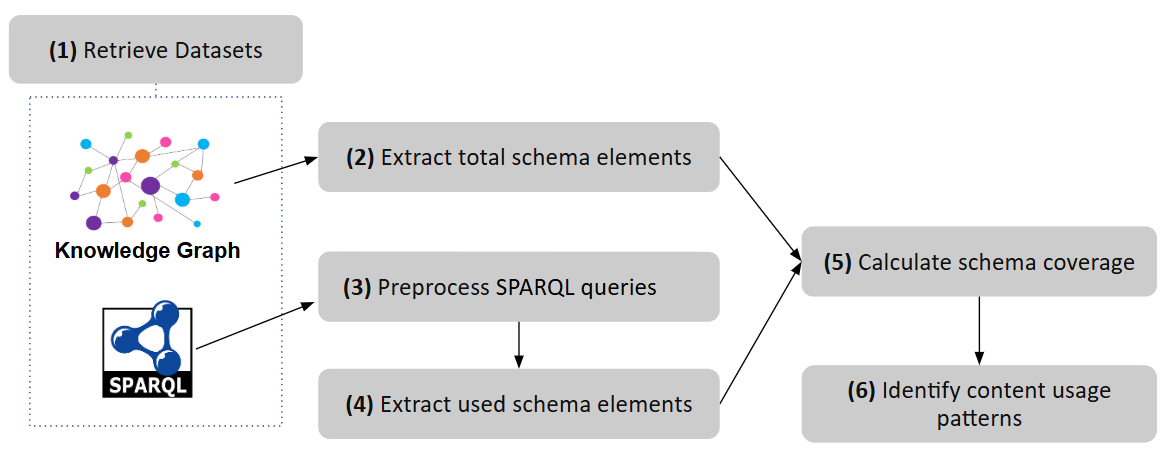
\includegraphics[width=0.8\textwidth]{image14.png} 
    \caption{Workflow of the proposed method }
    \label{fig:l1}
\end{figure}


\subsection{Datasets}

\textbf{RDF KGs.} Given that our analysis spans a period of Wikidata SPARQL query logs from 2017 to 2018, we downloaded a version of Wikidata from 2017 and 2018, as these are the closest versions available to the log period. This ensures maximum alignment of schema and query logs. We use both versions to investigate how the SPARQL schema coverage changes with the evolution of the Wikidata KG. We downloaded two versions of Wikidata from the Internet Archive\footnote{Wikidata version 2017: \url{https://archive.org/download/wikibase-wikidatawiki-20170821} and Wikidata version 2018: \url{https://archive.org/download/wikibase-wikidatawiki-20180205}}, and hosted them on Blazegraph on a local server. 

For Bio2RDF KG \cite{belleau2008bio2rdf}, the analysis covers two periods of SPARQL query logs: one beginning in 2013 and the other in 2019. However, due to the unavailability of datasets from these years, we instead use the current 2024 public endpoint\footnote{\url{https://Bio2RDF.org/sparql/}}. Since the live endpoint may change over time, we save and release the exact set of types and predicates extracted from the 2024 endpoint and used in our analysis.

\textbf{SPARQL Query Logs. }
The query logs are primarily retrieved from the Linked SPARQL Queries Dataset (LSQ) 2.0 endpoint\footnote{\url{https://lsq.data.dice-research.org/sparql}} using the query illustrated in Listing \ref{lst:SPARQL_query}. This query extracts the text and execution time of queries from 24 datasets in LSQ 2.0 \cite{stadler2024lsq}, including 23 Bio2RDF datasets and one Wikidata query dataset.
Furthermore, we downloaded Bio2RDF logs from Dumontier’s lab repository\footnote{\url{https://download.dumontierlab.com/Bio2RDF/logs/}} and Wikidata queries (all queries and organic queries for interval 1 and interval 7) from the International Center for Computational Logic\footnote{\url{https://iccl.inf.tu-dresden.de/web/Wikidata_SPARQL_Logs/en}}.

Among the many KGs available through LSQ, we selected Bio2RDF for two reasons. First, it is a domain-specific (life-sciences) KG with a compact, OWL-style schema, which contrasts sharply with the broad, general-purpose, and very large schema of Wikidata; comparing the two lets us study usage across two extremes of schema scale and design. Second, large Bio2RDF logs are available to us, including logs that retain user-agent information and therefore permit the organic/robotic split. The number of queries per dataset is substantial (ranging from $\sim$0.2 million to $\sim$81 million; full counts are reported in Tables~\ref{tab:1} and \ref{tab:2}).

The interval boundaries are not chosen by us; they are inherited from the upstream releases. For Wikidata, intervals~1 and~7 are the two intervals of the ICCL/Dresden release that provide the organic/robotic partition together with sufficient volume, and they bracket an approximately one-year span (2017 vs.\ 2018) that aligns with the 2017 and 2018 KG dumps we host. For Bio2RDF, the 2013 and 2019 periods correspond to the two log dumps available (LSQ and the Dumontier-lab repository, respectively). Because these periods differ in length, all frequency analyses use \emph{time-normalized} counts (Section~\ref{sec:s61}), where one month is defined as a fixed 30-day period and a log's duration in months is computed as $(\text{end date}-\text{start date})/30$ days.


\begin{center}
\begin{minipage}{0.8\textwidth}  % Adjust the width as needed
\begin{lstlisting}[label={lst:SPARQL_query},linewidth=\linewidth, caption={The templated SPARQL query against the LSQ SPARQL endpoint to retrieve SPARQL queries for selected datasets.}]
PREFIX lsqv: <http://lsq.aksw.org/vocab#>
PREFIX prov: <http://www.w3.org/ns/prov#>

SELECT DISTINCT ?text ?timeStamp

FROM <http://lsq.aksw.org/{dataset_name}>

WHERE {
    ?query  lsqv:text          ?text .
    ?query  lsqv:hasRemoteExec ?re .
    ?re     prov:atTime        ?timeStamp .
}
\end{lstlisting}
% \label{lst:SPARQL_query}
\end{minipage}
\end{center}


We implemented the method in \cite{bielefeldt2018practical, malyshev2018getting} to classify queries as organic or robotic based on the agent who executed the query. The Bio2RDF log2019 dataset includes user agent information, enabling us to generate the Bio2RDF organic and robotic log2019 subsets. The criteria used for classification are as follows:

\textbf{Organic:} If the user agent string contains indicators commonly associated with web browsers, such as "Mozilla," "Chrome," "Safari," "Firefox," "Edge," or "Opera," it was classified as organic. These are typically representative of human users.

\textbf{Robotic:} Entries whose user agent lacks browser indicators were classified as robotic. In practice these agents carry terms such as "Apache," "HttpClient," "Crawler," "sparqlwrapper," "python," or "Java," which are linked to automated scripts or bots; however, the operational rule is the complement of the organic test (any non-browser, non-empty agent), so that agents not matching a fixed keyword list are still treated as robotic rather than discarded.

\textbf{No agent:} A small number of entries carry no user-agent string and cannot be assigned to either class; they are excluded from the organic/robotic split.

\subsection{Extracting Total Schema Elements}

In this study, the \emph{schema} of a KG is the set of its distinct \emph{types} (classes) and \emph{predicates}. A \emph{schema element} is one such type or predicate. A \emph{schema (type) pattern} is a triple pattern at the schema level, $(\text{type}_1,\ \text{predicate},\ \text{type}_2)$, i.e., an edge of the schema graph connecting instances of $\text{type}_1$ to instances of $\text{type}_2$ via $\text{predicate}$. We extract these schema elements directly from the data of each KG, because neither KG ships a single authoritative schema document that matches the deployed data.

Listing~\ref{lst:l2} presents the pseudocode and queries used to extract the schema of a KG. The extraction process involves two main queries. Query~1 (line 7 in Listing~\ref{lst:l2}) retrieves all types, while Query~2 (line 13 in Listing~\ref{lst:l2}) extracts relationships between instances of different types. Using two optimized queries instead of a single complex query improved performance in large KGs, preventing timeout issues. For a few types, Query~2 still encountered timeouts due to the high number of instances and relationships; in such cases, simplified queries were used to mitigate the issue.

For Bio2RDF and Wikidata, the properties used in these queries differ. In Bio2RDF, \texttt{rdf:type} and \texttt{rdfs:subClassOf} are used, whereas Wikidata employs \texttt{wdt:P31} (\emph{instance of}) and \texttt{wdt:P279} (\emph{subclass of}) as their equivalents. Additionally, since Wikidata lacks subgraphs in its architecture, the ``Graph'' component is omitted from Query~2 when applied to Wikidata. For Bio2RDF we additionally keep only IRIs that match the Bio2RDF vocabulary template \url{http://Bio2RDF.org/DATASET_vocabulary:SCHEMA_ELEMENT} (excluding the generic \texttt{:Resource}), which yields OWL-style class and property IRIs.

\paragraph{\textbf{What counts as a ``class'' in Wikidata, and how it is used.}} We distinguish two schema modeling styles that matter for measurement. In an \emph{OWL-style} KG, classes and properties are dedicated vocabulary IRIs, disjoint from the instance data, and a class is not itself a legitimate value of a property; Bio2RDF and DBpedia are of this kind, and their schemas are unambiguous to extract. In an \emph{item-based} KG, there is no formal class/instance separation: the same kind of resource serves as both, so an entity may act as a class in one triple and as an ordinary data value in another. Wikidata is of this kind. Its ``classes'' are ordinary items, distinguished only by being used as the object of \texttt{wdt:P31} (\emph{instance of}) or \texttt{wdt:P279} (\emph{subclass of}); defining a Wikidata class is genuinely contested \cite{brasileiro2016applying,piscopo2018who,patelschneider2024class}. In the logs we analyse, the \emph{same} item is far more often referenced in queries as a property \emph{value} than as a class: e.g.\ \texttt{Q33999} (\emph{actor}) as the value of \texttt{P106} (\emph{occupation}), or \texttt{Q142} (\emph{France}) as the value of \texttt{P27} (\emph{country of citizenship}). A faithful usage analysis must therefore distinguish the \emph{position} in which an element is referenced. We call an entity reference \emph{class-position} when it is the object of \texttt{wdt:P31}/\texttt{wdt:P279} (or of a property path involving them, such as \texttt{wdt:P31/wdt:P279*}), and \emph{value-position} otherwise. Conflating the two, as a naive ``type coverage'' does, counts value usage as though it were schema usage; we therefore report the split (Section~\ref{sec:classvalue}). This distinction does not arise for Bio2RDF, whose vocabulary classes are not used as property values. We additionally distinguish \emph{instantiated} classes (objects of \texttt{wdt:P31}, $\geq 1$ instance) from purely hierarchical or uninstantiated items. These distinctions are central to interpreting the Wikidata coverage numbers and to the discussion of what ``schema coverage'' means for an item-based KG (Section~\ref{s5}).

\paragraph{\textbf{Worked example.}} Consider the two example queries from the Wikidata Query Service. The first, \texttt{SELECT ?cat WHERE \{ ?cat wdt:P31 wd:Q146 \}} (house cats), references the predicate \texttt{P31} and the type \texttt{Q146}; both are extracted as used schema elements. The second, \texttt{?horse wdt:P31/wdt:P279* wd:Q726} (horses and their subclasses), references the predicates \texttt{P31} and \texttt{P279} and the type \texttt{Q726}; these three are extracted. Note that the \texttt{wdt:P279*} closure means the query also retrieves subclasses of horse (e.g.\ \emph{racehorse}, \texttt{Q2442470}), but those subclass IRIs are \emph{not} written in the query text and are therefore not counted as explicitly referenced (we return to this distinction in Section~\ref{s3}.4 and Section~\ref{s5}).

The schema for any Bio2RDF dataset follows a specific URL template: \url{http://Bio2RDF.org/DATASET_vocabulary:SCHEMA_ELEMENT}. Therefore, any URLs retrieved from query execution that do not adhere to this template are excluded from the final schema elements set. \DIFaddbegin \DIFadd{We apply this filter to predicates as well as to types. This matters in practice: extracting predicates with the pattern }\texttt{\DIFadd{?s\,a\,?t\,.\ ?s\,?p\,?o\,.\ ?o\,a\,?t'}} \DIFadd{also captures statements }\emph{\DIFadd{about}} \DIFadd{the vocabulary, such as }\texttt{\DIFadd{sgd\_vocabulary:Resource\,rdf:type\,owl:Class}}\DIFadd{, which would otherwise admit four W3C terms (}\texttt{\DIFadd{rdf:type}}\DIFadd{, }\texttt{\DIFadd{rdfs:subClassOf}}\DIFadd{, }\texttt{\DIFadd{owl:sameAs}}\DIFadd{, }\texttt{\DIFadd{owl:sourceIndividual}}\DIFadd{) into the Bio2RDF schema. Those terms are not Bio2RDF vocabulary, and are not elements its maintainers can document, redesign, or deprecate, which are the decisions this measurement is meant to inform. Excluding them also keeps the three KGs on the same footing, since the Wikidata and DBpedia universes contain only their own vocabulary.
}\DIFaddend 


\begin{center}
\begin{minipage}{0.76\textwidth} % Adjust width here (e.g., 0.9 for 90% of text width)
\begin{lstlisting}[label={lst:l2},caption={Pseudocode to extract KG schema. KG schema extraction is consist of two queries, Query 1 and Query 2.}]
for graph in the KG:
        for each property in ['type_property', 'subclass_property']:
            Execute Query_1 to get subject_types
            for each subject_type and property in ['type_property', 'subclass_property']:
                execute Query_2 
                
Query_1:
SELECT DISTINCT ?subject_type
    WHERE {
        GRAPH <{graph}> {
            ?s {property} ?subject_type . } }

Query_2:
SELECT DISTINCT subject_type ?p ?object_type
WHERE {
    GRAPH <{graph}> {
        ?s {property} {subject_type} .
        ?s ?p ?o .
        ?o {property} ?object_type .  }} 
                    
\end{lstlisting}
\end{minipage}
\end{center}

\subsection{Preprocessing SPARQL Queries}

We extract unique SPARQL queries and store them along with their respective execution counts. Two queries are considered identical when their text is identical after collapsing runs of whitespace (spaces, tabs, and newlines) to a single space and trimming leading/trailing whitespace; we do not otherwise reformat the queries at this stage. We count over \emph{unique} queries because our questions concern the \emph{diversity} of schema elements that users and tools query, and deduplication prevents a small number of very high-frequency automated queries from dominating the distribution. We note that repetition is itself a meaningful signal of demand; deduplication is a deliberate choice to measure intent diversity rather than execution volume, and a complementary volume-weighted analysis is a natural extension. Before parsing, we preprocess the queries to ensure proper syntax and facilitate accurate parsing. First, we incorporate essential RDF syntax prefixes (such as \texttt{rdf}, \texttt{rdfs}, and \texttt{owl}) since some queries lack explicit prefix declarations. While Virtuoso pre-registers these prefixes—allowing users to omit them—our parser, 'sparqljs'\footnote{https://www.npmjs.com/package/sparqljs}, does not support this feature. Therefore, we add the necessary prefixes to all queries to ensure proper parsing.

Next, we normalize the queries for parsing. Crucially, this normalization is performed \emph{before} deduplication, so that queries differing only in incidental HTTP artifacts collapse to a single unique query. Specifically, we (i) fully percent-decode the query text; (ii) remove the trailing chain of HTTP query-string parameters that the log capture appended to the SPARQL text (queries were submitted as \texttt{GET /sparql?query=<SPARQL>\&format=...\&timeout=...\&callback=...}); we strip a terminal run of \texttt{\&key=value} segments, anchored to the end of the string so that IRIs containing \texttt{\&} mid-query are not affected; and (iii) collapse runs of whitespace.


After preprocessing, we parse the queries using \texttt{sparqljs}, a SPARQL~1.1 parser implemented in JavaScript, to eliminate queries that are not syntactically valid and to obtain the parse tree of each query for content extraction. All validity counts and all used-schema-element counts reported in this paper are produced by this \texttt{sparqljs} path. Our released code additionally implements two alternative back-ends, \texttt{rdflib} (Python) and \texttt{pyoxigraph} (Rust), which we use only as an independent check that the validity rates are not an artifact of a single parser (Section~\ref{s4}.3). A parse tree represents the syntactic structure of a query, breaking it down into its components, such as subjects, predicates, and objects. We standardize variable names, as demonstrated in Figure \ref{fig:l2}. Three equivalent queries that differ only in their variable names e.g., ?drug, ?compound, and ?s1, are standardized to ?var1. We distinguish variables from actual entities by substituting variable names with placeholders like 'varX'. The same preprocessing and variable standardization are applied identically to both the Bio2RDF and Wikidata logs. The output of this preprocessing is unique, normalized, valid queries.

\begin{figure}
    \centering
    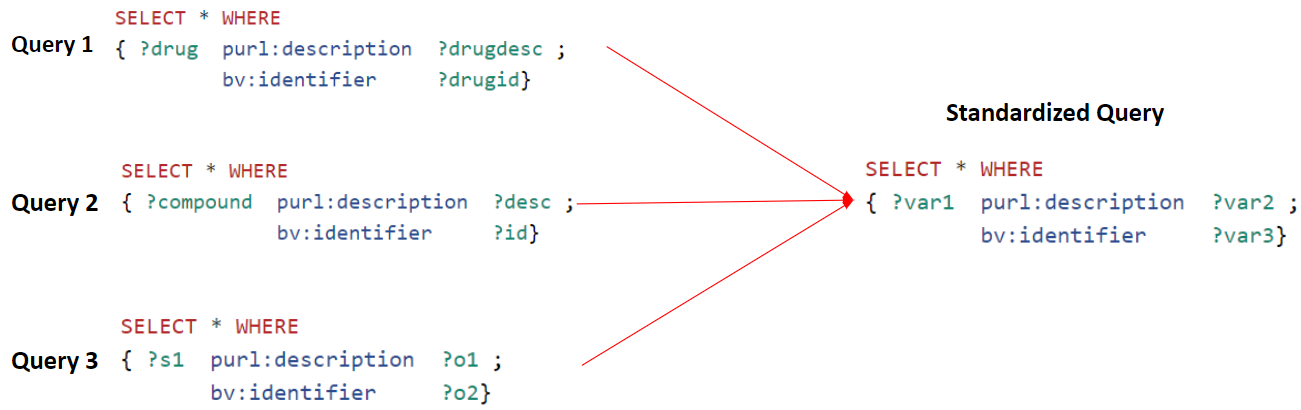
\includegraphics[width=0.8\textwidth]{image17.png} 
    \caption{Variable standardization. ?drug, ?compound, and ?s1, are standardized to ?var1.}
    \label{fig:l2}
\end{figure}
\subsection{Extracting Used Schema Elements }\label{sec:used}
We write a Python script to extract ``used schema elements'' from the parse trees of the queries. We first identify the subject, predicate, and object IRIs within each query's parse tree. Then, we determine the intersection of these IRIs with the total schema elements that were retrieved earlier.

\paragraph{\textbf{What we mean by ``used''.}} Throughout, a schema element is counted as \emph{used} if it is \emph{explicitly referenced}, i.e., its IRI is written in the query text, the \emph{explicit usage} notion introduced in Section~\ref{s1}. We deliberately adopt this explicit-reference notion rather than a closure- or answer-based (\emph{semantic}, effective) one. As illustrated by the horse example in Section~\ref{s3}.2, a query containing \texttt{wdt:P31/wdt:P279* wd:Q726} explicitly references only \texttt{P31}, \texttt{P279}, and \texttt{Q726}; the subclasses of horse that the property path traverses at evaluation time (e.g.\ \emph{racehorse}) contribute to the \emph{answers} but are not named in the query, and a similar effect arises with property hierarchies. Explicit reference is the appropriate notion for this paper's motivations: documentation, schema and interface design, autocomplete, and deprecation decisions all act on the elements that users and tools actually \emph{write}, not on the transitive closure a query happens to traverse. We quantified how often the two notions could diverge by measuring property-path usage. Property paths of any kind appear in only about 1\% of valid Bio2RDF organic queries (98 of 8,140), but in 21.1\% of Wikidata organic queries in 2017 (18,705 of 88,491) and 13.7\% in 2018 (25,351 of 185,443); restricting to the transitively-traversing \texttt{*}/\texttt{+} operators, which could pull in additional schema elements, these operators appear in 16.6\% of Wikidata organic queries in 2017 (14,696 of 88,491). The explicit-reference and closure-based notions therefore coincide for nearly all Bio2RDF queries, whereas for Wikidata a non-trivial fraction of queries traverse the subclass hierarchy that a closure-based notion would additionally credit.

We can bound this divergence directly. In the 2017 organic queries of Wikidata, the subclass-traversing paths (\texttt{wdt:P279*}, \texttt{wdt:P31/wdt:P279*}) are anchored at 1,276 distinct classes; the transitive subclass closure of those anchors, computed from the 2017 dump's 2.08M \texttt{P279} edges, spans 64,843 of the KG's $\sim$103,000 classes, of which 62,410 are not named explicitly. A closure/answer-based ``effective usage'' notion would therefore credit up to those 62,410 additional types, raising organic coverage from $\sim$4\% to $\sim$62\%, a $+60$ percentage-point swing. Crucially, this bound is dominated by a handful of queries anchored at near-root classes: \texttt{wdt:P279*} from \emph{entity} (\texttt{Q35120}) alone, used in just \DIFdelbegin \DIFdel{13 }\DIFdelend \DIFaddbegin \DIFadd{12 }\DIFaddend queries, has a closure of 64,356 classes, and \emph{concept} (\texttt{Q151885}) 49,828, whereas typical anchors are small (\emph{city} 96, \emph{film} 94, \emph{organization} 3,538). A closure-based metric is thus not merely harder to compute but ill-behaved on an item-based KG: a single query rooted at \emph{entity} would mark most of the ontology as ``used,'' conflating \emph{queried} with \emph{reachable in principle}. This is positive evidence for the explicit-reference choice; a principled, partially-credited closure measure remains future work (Section~\ref{s5}).
\DIFdelbegin %DIFDELCMD < \begin{comment}%DIFDELCMD < 
%DIFDELCMD < 
%DIFDELCMD < Where are these 13 queries made available? After examining the code, scripts, and datasets in the GitHub repository, I could not identify a file containing them. It would be useful to provide these 13 queries in a supplementary file and reference that file here to improve transparency and reproducibility.
%DIFDELCMD < 
%DIFDELCMD < \end{comment}
%DIFDELCMD < %%%
\DIFdelend 

\subsection{Calculating Schema Coverage}
Equation \ref{eq:1} was used to calculate the SPARQL Schema Coverage (SC). This metric quantifies the proportion of the KG schema that is used by user queries. SC is the ratio of Used Schema Elements (USE) to Total Schema Elements (TSE) in the KG, multiplied by 100 to express the result as a percentage. The TSE represents the count of all distinct types and predicates in the KG, while the USE denotes the count of those classes and predicates found in user SPARQL query logs. We obtained the values for USE and TSE from the results of the previously described steps. Coverage is always reported against a \emph{clearly delimited reference set}: the numerator and denominator are derived from the same set of subgraphs (Section~\ref{s4}.1), and we report types and predicates separately (Table~\ref{tab:4}) rather than only their sum. Because the type sets of Bio2RDF and Wikidata are constructed differently (OWL-style vocabulary IRIs vs.\ the data-driven \texttt{wdt:P31}/\texttt{wdt:P279} operationalization of Section~\ref{s3}.2) and differ in scale by roughly two orders of magnitude, coverage percentages are meaningful \emph{within} a KG (across query types and time) but should not be read as a direct cross-KG comparison.
\begin{equation}
SC (\%) = \left( \frac{USE}{TSE} \right) \times 100
\label{eq:1}
\end{equation}

\subsection{Identifying Content Usage Patterns}\label{sec:s6}
Up to this point, we have introduced a method for calculating SPARQL schema coverage, which measures the proportion of schema elements in a KG that are queried. However, this metric alone does not reveal how frequently individual schema elements are used or whether their usage is consistent over time. Step six involves analyzing the frequency distribution of the schema elements, identifying frequently used elements, and detecting commonalities in robotic and organic logs, or across different time periods. Additionally, we apply statistical tests, including the Wilcoxon signed-rank test and Spearman's rank correlation coefficient, to assess the consistency and changes in the frequency and ranking of schema element usage over time. The following sections provide a detailed explanation of these methods, with the findings presented in the Results section.

\subsubsection{Frequency Distribution of Schema Elements}\label{sec:s61}
To analyze and compare the frequency distributions of schema elements across multiple datasets, we normalize the usage count of each element to account for varying time intervals. We calculate the monthly frequency of each element by dividing its total count by the log collection period expressed in months (Equation \ref{eq:2}). Here one month is a fixed 30-day period, so the normalized count has units of \emph{uses per 30-day month}. To reduce skewness and enhance interpretability, we apply a logarithmic transformation ($\log_{10}$) to these normalized counts. Finally, we visualize the normalized frequency distribution of schema elements across different datasets to facilitate comparison.

\begin{equation}
\text{Normalized count} = \frac{\text{Total count}}{\text{log collection period}}
\label{eq:2}
\end{equation}

Before comparing the two intervals statistically, we must decide whether a parametric (normality-assuming) test is appropriate. The Shapiro--Wilk test (Equation~\ref{eq:shapiro}) assesses whether a sample plausibly comes from a normal distribution; we use it purely as a precondition check. We apply it to the per-element \emph{change} in normalized usage frequency between the two intervals (defined below). Thus, the normality assumption concerns the distribution of these numerical differences.

\begin{equation}
SW = \frac{\left( \sum_{i=1}^n a_i x_i \right)^2}{\sum_{i=1}^n (x_i - \bar{x})^2}
\label{eq:shapiro}
\end{equation}

where the \( x_i \) are the ordered sample values, \( \bar{x} \) is the sample mean, and the \( a_i \) are the Shapiro--Wilk coefficients, i.e., tabulated constants derived from the expected values and covariances of the order statistics of a standard-normal sample of size \( n \). In our case each \( x_i \) is, for one schema element common to both intervals, the change in its normalized monthly usage frequency from the first interval to the second (interval-2 value minus interval-1 value).


The test returned $p \approx 0$ for both the Wikidata and Bio2RDF interval pairs, so the per-element changes are not normally distributed. We therefore use the non-parametric Wilcoxon signed-rank test (Equation~\ref{eq:wilcoxon}), which compares the same schema element measured in two intervals (a paired design) without assuming normality, to test whether usage frequencies shifted significantly between the two intervals.

\begin{equation}
W = \sum_{i=1}^n \text{sign}(d_i) R_i
\label{eq:wilcoxon}
\end{equation}

where \(d_i\) is the difference between the usage frequency of schema elements (in two intervals), \( \text{sign}(d_i) \) is the sign of \(d_i\), and \(R_i\) is the rank of the absolute differences.


\paragraph{\textbf{Changes in Used Schema Element Ranking.}}
The Wilcoxon test addresses changes in usage \emph{magnitude}; we separately ask whether the relative \emph{popularity ranking} of schema elements is stable over time. We rank elements by their normalized usage frequency within each interval (rank 1 = most frequently used) and compute Spearman's rank correlation coefficient (\( \rho \)) (Equation~\ref{eq:4}) between the two rankings. Spearman's \( \rho \) is the Pearson correlation of the ranks; it summarizes in a single number in \([-1,1]\) whether elements that were popular in one interval remained popular in the other, and it is distribution-free, which suits our non-normal data. Here \( d_i \) is the difference between the ranks of schema element \( i \) in the two intervals, and \( n \) is the number of common schema elements \cite{spearman1961proof}. We use Spearman's \( \rho \) as a compact measure of temporal \emph{stability}, complementing the Wilcoxon test.
\begin{equation}
\rho = 1 - \frac{6 \sum d_i^2}{n(n^2 - 1)}
\label{eq:4}
\end{equation}

% To measure the proportion of schema element pairs that maintain their relative rank ordering between the two intervals, we calculate the concordance index (equation~\ref{eq:5}), where concordant pairs are defined as a pair of schema elements \( (i, j) \) that their relative ranks are the same in both intervals.

% \begin{equation}
%     \text{C-index} = \frac{\text{Number of concordant pairs}}{\text{Total number of pairs}}
%     \label{eq:5}
% \end{equation}


\subsubsection{Frequent Schema Elements} \label{sec:s62}
We analyze the most frequently queried schema types from robotic and organic logs of Wikidata and Bio2RDF to identify common elements that persist across different time intervals and log types. This focus on the most frequent elements is similar in spirit to the predicate-frequency analysis of Bonifati et al.\ \cite{bonifati2019navigating}, to which we add the temporal and organic/robotic dimensions. While our ranking analysis of all schema elements reveals broad usage dynamics and temporal shifts, we're particularly interested in determining whether a subset of frequently accessed elements remains consistently popular over time, indicating their significance as "core" elements of the KG. The presence of a stable core across the datasets would suggest that these elements are central to the KG’s utility, regardless of the query time or type. This frequent-element analysis is computed over schema \emph{types} (classes); predicates, whose frequency distribution is dominated by a few generic relations, are analyzed separately. To investigate the stable core, we first examine the top 10 schema types in each dataset, as they represent the most frequently queried components, as well as the top 50 types. The top 50 threshold strikes a balance by providing a more comprehensive view of usage patterns compared to the top 10 while still avoiding the inclusion of many low-frequency types. For example, in Wikidata 2017, the frequency for types ranked 51 to 3560 ranges from 149 to 1, whereas the top 50 types have frequencies between 6,962 and 150. To analyze schema usage patterns, we visualize frequently queried schema elements and identify common elements across datasets, log types, and time intervals. This approach aims to determine whether there is a set of core schema elements that drives query activity in these KGs.


\paragraph{\textbf{Pairwise Schema Type Usage of Bio2RDF.}}
Bio2RDF consists of 26 interconnected subgraphs, each representing a distinct dataset with its own vocabulary. These subgraphs are linked through various predicates. For example, the \url{ctd_vocabulary:Gene-Disease-Association} type from the "ctd" subgraph and the \url{ncbigene_vocabulary:Resource} from the "ncbigene" subgraph are linked by the predicate \url{ctd_vocabulary:gene}, establishing a relationship between the two elements. A typical triple pattern representing the connection between two distinct subgraphs is: \sloppy \texttt{?schema\_Type\_from\_first\_subgraph ?predicate ?schema\_Type\_from\_second\_subgraph}. This relationship is referred to as a "pairwise schema type pattern."

Bio2RDF’s subgraph organization enables an analysis of how frequently queries capture relationships between schema types from different subgraphs. However, since Wikidata does not have an explicit subgraph structure, this type of analysis is not applicable to its dataset. To investigate this type of usage, we conduct an experiment comparing Bio2RDF query logs from 2013 and 2019 to determine how often datasets (or subgraphs) were integrated in queries to retrieve more complex information. The approach consists of two main steps:

\textbf{Identifying total pairwise schema type patterns.} We extract all possible pairwise schema type patterns from the Bio2RDF schema, covering 17 subgraphs in log\_2013 and 26 subgraphs in log\_2019.


\textbf{Identifying pairwise schema type pattern occurrences in logs.} We analyze the triple patterns within queries to identify occurrences of these pairwise schema type patterns. For each dataset, we construct a matrix where both rows and columns represent schema type subgraphs. Each cell in the matrix corresponds to a specific pair of subgraphs, and its value indicates the frequency of the pattern in the queries.
By conducting this analysis, we aim to discover how often queries integrate information across Bio2RDF subgraphs and how this usage has evolved over time.

\section{Results}\label{s4}
In this section, we describe the results of the various steps in the method, including the retrieval of datasets, the pre-processing of SPARQL queries, the extraction of all schema elements, the extraction of the schema elements used, the calculation of the SPARQL schema coverage, and the analysis of usage patterns.

\subsection{Dataset Retrieval }
Table \ref{tab:1} provides an overview of the datasets retrieved for analysis, including the logs from Bio2RDF and Wikidata KGs for multiple periods and query types. We use a single naming convention of the form \emph{KG-agentType-period[-interval]}; for example, \emph{Bio2RDF-all-2013} is the full 2013 Bio2RDF log and \emph{Wikidata-organic-2017-int1} is interval~1 of the 2017 Wikidata organic log. Because most analyses evaluate a log against a specific KG version, we extend the same convention with the version it is paired with, written \emph{log\textlangle period\textrangle\_kg\textlangle version\textrangle}: for instance \emph{Bio2RDF-all-log2013\_kg2024} denotes the \emph{Bio2RDF-all-2013} log evaluated against the 2024 Bio2RDF schema. Tables~\ref{tab:1}--\ref{tab:5} and the figure panels use these two forms throughout, the plain form where only the log matters and the paired form where the KG version does. The \emph{Bio2RDF-all-2013} log originates from LSQ and spans 16.79 months, from May 2013 to September 2014, containing 31,950,877 queries. This LSQ-derived dataset lacks user-agent information and only includes the \texttt{lsqv:hostHash} property, an anonymized hash of the host or IP address issuing each query; the LSQ release therefore cannot itself be split into organic and robotic. To recover that split for the 2013 era we additionally obtained the \emph{raw} Bio2RDF server access log (the upstream source from which LSQ was built, spanning May 2013--September 2015), which retains user agents; we use it to characterize 2013-era organic vs.\ robotic traffic in Section~\ref{sec:bio2013}. The second dataset, \emph{Bio2RDF-all-2019}, covers a longer period of 29.93 months, from January 2019 to July 2021. It comprises 3,880,960 log entries. Of these, 3,212 are server-side log lines that contain no SPARQL query, leaving 3,877,748 SPARQL queries. This dataset retains user-agent information, allowing us to separate robotic (3,816,776) and organic (56,736) queries; a further 7,427 queries lack user-agent information and are excluded from the split.

Wikidata logs contain both organic and robotic queries. The \emph{Wikidata-organic-2017-full} log spans 9.43 months, from June 2017 to March 2018, and consists of 3,298,254 organic queries. The shorter intervals used for the temporal comparison each cover 0.88 months: \emph{Wikidata-organic-2017-int1} and \emph{Wikidata-organic-2018-int7} comprise 192,331 and 872,556 organic queries, respectively, while \emph{Wikidata-robotic-2017-int1} and \emph{Wikidata-robotic-2018-int7} contain 59,355,579 and 81,339,186 robotic queries, respectively.

\begin{table}[h!]
\centering
\caption{Results of the data retrieval step. Datasets follow the naming convention \emph{KG-agenttype-period[-interval]}; ``All'' denotes the union of organic and robotic queries (not a superset of any single row).}
\label{tab:1}
\begin{tabular}{l|r|l|r} 
\hline
\textbf{Dataset} & \#\textbf{Queries} & \textbf{log collection period} & \textbf{Duration (months)} \\ \hline
Bio2RDF All log2013 & 31,950,877 & 2013-05-05 to 2014-09-28 & 16.79 \\ 
Bio2RDF All log2019 & 3,880,960  & 2019-01-07 to 2021-07-06 & 29.93 \\ 
Bio2RDF robotic log2019 & 3,816,776  & 2019-01-07 to 2021-07-06 & 29.93 \\ 
Bio2RDF organic log2019 & 56,736 & 2019-01-07 to 2021-07-06 & 29.93 \\ 
Wikidata All organic log2017 & 3,298,254 & 2017-06-11 to 2018-03-25 & 9.43 \\ 
Wikidata robotic log2017 & 59,355,579 & 2017-06-12 to 2017-07-09 & 0.88 \\ 
Wikidata robotic log2018 & 81,339,186 & 2018-02-26 to 2018-03-25 & 0.88 \\ 
 Wikidata organic log2017&
192,331&
2017-06-12 to 2017-07-09&
0.88\\
Wikidata organic log2018&
872,556&
 2018-02-26 to 2018-03-25&
0.88\\
\hline
\end{tabular}
\end{table}

During our analysis in 2024, the Bio2RDF SPARQL endpoint contained 26 subgraphs/datasets. However, the Bio2RDF log2013 and Bio2RDF log2019 datasets do not contain query logs corresponding to all 26 subgraphs. Figures \ref{fig:l3} and \ref{fig:l4} provide details through Venn diagrams: Figure \ref{fig:l3} illustrates the overlap between the Bio2RDF log2013 datasets and the KG subgraphs, while Figure \ref{fig:l4} represents the Bio2RDF log2019 datasets compared to the KG subgraphs in the 2024 endpoint. This comparison highlights the importance of using a consistent reference set when calculating schema coverage (Equation \ref{eq:1}). That is, the numerator and denominator (i.e., used and total schema elements) should be derived from the same set of datasets, ensuring alignment between KG subgraphs and log datasets.

The Venn diagram in Figure \ref{fig:l3} compares the datasets included in Bio2RDF log2013 with the subgraphs in Bio2RDF KG2024. The left oval represents datasets unique to Bio2RDF log2013. The overlapping section in the center lists 17 datasets common to both Bio2RDF log2013 and Bio2RDF KG2024. The right oval represents datasets unique to Bio2RDF KG2024.


The Venn diagram in Figure \ref{fig:l4} compares the datasets included in Bio2RDF log2019 with the subgraphs in Bio2RDF KG2024. The left oval represents datasets unique to Bio2RDF log2019. The overlapping section in the center lists 22 datasets common to both Bio2RDF log2019 and Bio2RDF KG2024. The right oval represents datasets unique to Bio2RDF KG2024. 

The  dataset "Bio2RDF" in log2019 refers to the logs of a general endpoint for all subgraphs and may include queries to the HP, ECO, APO, and GO subgraphs. This is because, historically, Bio2RDF maintained a distinct SPARQL endpoint for each subgraph. Later, a single general endpoint was introduced to host all subgraphs for querying.


\begin{figure}
    \centering
    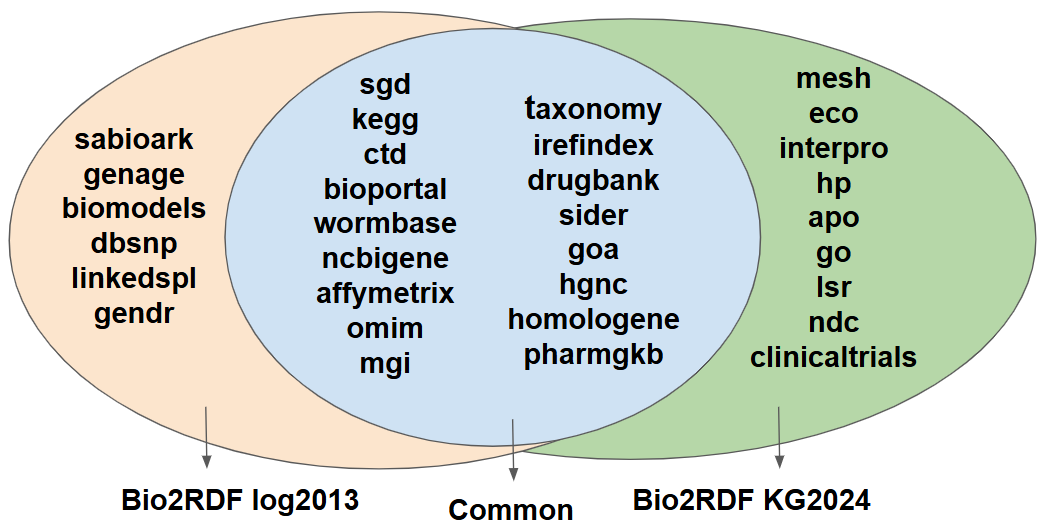
\includegraphics[width=0.53\textwidth]{image9.png} 
    \caption{Venn diagram illustrating the overlap  between the Bio2RDF log2013 datasets and the Bio2RDF KG 2024
}
    \label{fig:l3}
\end{figure}

\begin{figure}[htbp]
    \centering
    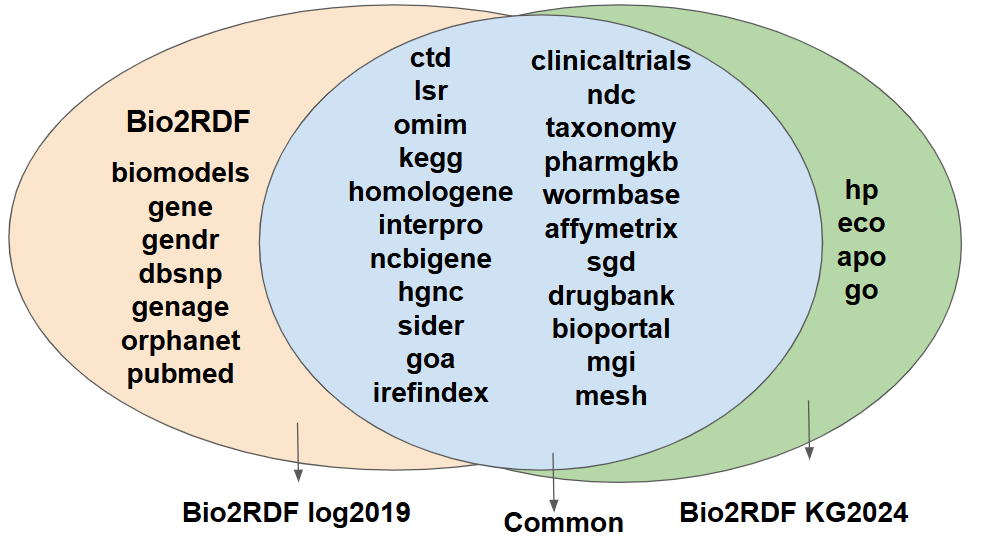
\includegraphics[width=0.55\textwidth]{image8.png} 
    \caption{ Venn diagram illustrating the overlap between the Bio2RDF log2019 datasets and the Bio2RDF KG 2024
}
     \label{fig:l4}
\end{figure}


\subsection{Extracting Total Schema Elements}
Table \ref{tab:3} presents the statistics of total schema elements across different KG versions. Initially, the Bio2RDF schema comprised 166,444 unique types. After excluding types that do not adhere to the template \url{http://Bio2RDF.org/DATASET_vocabulary:SCHEMA_ELEMENT}',' 545 types remain. A further refinement, by excluding elements with the template \url{'http://Bio2RDF.org/DATASET_vocabulary:Resource,'} reduces the count to 350 types and \DIFdelbegin \DIFdel{195 }\DIFdelend \DIFaddbegin \DIFadd{191 }\DIFaddend predicates, distributed across 26 subgraphs within the Bio2RDF KG on the current endpoint (2024). Out of these 26 subgraphs, only 17 have corresponding query logs available in the Bio2RDF log2013 dataset, as depicted in Figure \ref{fig:l3}. These 17 subgraphs contain 270 types and \DIFdelbegin \DIFdel{129 }\DIFdelend \DIFaddbegin \DIFadd{125 }\DIFaddend predicates, in total \DIFdelbegin \DIFdel{399 }\DIFdelend \DIFaddbegin \DIFadd{395 }\DIFaddend schema elements.

As represented in Table \ref{tab:3}, the Wikidata KG version 2017 contains 103,380 types, whereas the Wikidata KG version 2018 contains 97,470 types, reflecting a reduction in the number of schema types. These results illustrate the variability in schema complexity with Wikidata exhibiting a larger and more diverse set of schema elements compared to Bio2RDF.
\begin{table}[ht]
\centering
\caption{Total schema elements Statistics per KG version}
\label{tab:3}
\DIFdelbeginFL %DIFDELCMD < \resizebox{\textwidth}{!}{
%DIFDELCMD < \begin{tabular}{l|r|r|r|r}
%DIFDELCMD < \hline
%DIFDELCMD < Source & Bio2RDF KG2024 (17 subgraphs) & Bio2RDF KG2024 (26 subgraphs) & Wikidata KG2017 & Wikidata KG2018 \\
%DIFDELCMD < \hline
%DIFDELCMD < Total number of distinct Elements & 399 & 545 & 104,314 & 98,462 \\
%DIFDELCMD < Number of distinct Types & 270 & 350 & 103,380 & 97,470 \\
%DIFDELCMD < Number of distinct Predicates & 129 & 195 & 934 & 992 \\
%DIFDELCMD < \hline
%DIFDELCMD < \end{tabular}
%DIFDELCMD < }
%DIFDELCMD < %%%
\DIFdelendFL \DIFaddbeginFL \resizebox{\textwidth}{!}{
\begin{tabular}{l|r|r|r|r}
\hline
Source & Bio2RDF KG2024 (17 subgraphs) & Bio2RDF KG2024 (26 subgraphs) & Wikidata KG2017 & Wikidata KG2018 \\
\hline
Total number of distinct Elements & 395 & 541 & 104,314 & 98,462 \\
Number of distinct Types & 270 & 350 & 103,380 & 97,470 \\
Number of distinct Predicates & 125 & 191 & 934 & 992 \\
\hline
\end{tabular}
}
\DIFaddendFL \end{table}


\subsection{Preprocessing SPARQL Queries}
Table \ref{tab:2} summarizes the number of queries (\#Queries), unique queries (\#Unique), queries with incorrect syntax (\#Failed to parse), and unique syntactically valid queries (\#Valid) across all datasets. The Bio2RDF~2019 rows differ most from the preliminary work \cite{mohammadi2024analyzing}: for \emph{Bio2RDF-all-2019}, the dataset also used there, the corrected parameter stripping yields 1{,}040{,}666 valid queries against 634{,}783 previously, because the appended HTTP query-string parameters had caused a large share of well-formed queries to be discarded.

We report the effect of the variable standardization described in Section~\ref{s3}.3, the last preprocessing step, on merging queries that differ only in variable naming and should therefore not count as distinct usage. Its effect is small in every log we measured: applying it to the valid queries reduces \emph{Bio2RDF-organic-2019} from 8{,}208 to 8{,}099 distinct query shapes (1.3\%), \emph{Bio2RDF-robotic-2019} from 1{,}034{,}833 to 1{,}034{,}754 (0.01\%), \emph{Wikidata-organic-2017-int1} from 88{,}514 to 88{,}116 (0.45\%), \emph{Wikidata-organic-2018-int7} from 185{,}478 to 184{,}934 (0.29\%), and the multi-million-query \emph{Wikidata-all-2017-int1} from 8{,}317{,}396 to 8{,}316{,}939 (0.01\%). Variable naming is therefore almost never the only difference between two logged queries.  In our pipeline, standardization assigns consistent variable names (e.g., \texttt{VAR1}, \texttt{VAR2}, \ldots), primarily to support the correct extraction of schema elements from the parse tree rather than deduplication.

% We reviewed the 416,896 queries in the Bio2RDF log 2019 that failed to parse. Approximately 300,000 of the 416,896 failures were simple templates with varying LIMIT and OFFSET values, as shown in Listing \ref{lst:third_list} 6 with a syntactic error. More than 1,819 of these queries were not SPARQL queries at all; rather, they were plain text, mostly in English. For example, one such message reads: "I love your blog... very nice colors \& theme. Did you make ...". Interestingly, the execution agent for these queries is Mozilla, rather than Java, Python, or any web crawler. Nine queries contained only the string "/sparql." 
% \begin{center}
% \begin{minipage}{0.76\textwidth} % Adjust width here (e.g., 0.9 for 90% of text width)
% \begin{lstlisting}[caption={The templated SPARQL query against the LSQ SPARQL endpoint to retrieve SPARQL queries for selected datasets.}]
% -- Query 1

%     SELECT ?r (COUNT(*) AS ?count) WHERE { ?r ?s ?o } 
%     OFFSET 177863205 LIMIT 1000 
%     GROUP BY ?rOFFSET 0 LIMIT 10000

%  -- Query 2

%     SELECT ?r (COUNT(*) AS ?count) WHERE { ?r ?s ?o } 
%     OFFSET 62950773 LIMIT 1000 
%     GROUP BY ?rOFFSET 0 LIMIT 10000

% -- Query 3

%     SELECT ?r (COUNT(*) AS ?count) WHERE { ?r ?s ?o } 
%     OFFSET 85005378 LIMIT 1000 
%     GROUP BY ?rOFFSET 0 LIMIT 10000

% \end{lstlisting}
% \label{lst:third_list}
% \end{minipage}
% \end{center}

\begin{table}[ht]
\centering
\caption{Results of parsing and validating the query logs, regenerated with the
corrected preprocessing (full HTTP query-string parameter stripping applied before
deduplication, base-IRI resolution of relative IRIs). \#Failed-to-parse $=$ \#Unique
$-$ \#Valid. \#Valid is computed with the \texttt{sparqljs} SPARQL~1.1 parser.
The Bio2RDF~2013 figures use the executed-query set (queries with a recorded remote
execution).}
\label{tab:2}
\begin{tabular}{l|r|r|r|r}
\hline
Dataset & \#SPARQL Queries & \#Unique & \#Failed to parse & \#Valid \\
\hline
Bio2RDF All log2013 & 31,950,877 & 1,519,681 & 2,521 & 1,517,160 \\
Bio2RDF All log2019 & 3,880,939 & 1,050,616 & 9,950 & 1,040,666 \\
Bio2RDF robotic log2019 & 3,824,203 & 1,040,356 & 5,525 & 1,034,831 \\
Bio2RDF organic log2019 & 56,736 & 12,579 & 4,439 & 8,140 \\
Wikidata All organic log2017 & 3,530,948 & 859,290 & 321 & 858,969 \\
Wikidata robotic log2017 & 59,355,579 & 8,234,089 & 20 & 8,234,069 \\
Wikidata robotic log2018 & 81,339,186 & 18,939,743 & 86 & 18,939,657 \\
Wikidata organic log2017 & 192,330 & 88,514 & 23 & 88,491 \\
Wikidata organic log2018 & 872,555 & 185,478 & 35 & 185,443 \\
\hline
\end{tabular}
\end{table}


We further examine the invalid queries in the Bio2RDF~2019 logs, providing further context for the validity counts reported in Table~\ref{tab:2}. We also evaluate whether the choice of parser affects the validity classification.

First, in the Bio2RDF~2019 logs, organic and robotic queries differ substantially in their validity rates. About 99.5\% of unique robotic queries parse, whereas a large fraction of unique organic entries are not SPARQL at all. Inspection of these entries shows injected non-SPARQL text, mostly blog-comment spam submitted to the public endpoint form (one entry reads ``I love your blog... very nice colors \& theme''), together with nine entries consisting only of the string \texttt{/sparql}. This reflects the use of an open web form on a public endpoint rather than a general characteristic of human querying. 


Second, some queries use Virtuoso-specific features, such as \texttt{bif:contains}, \texttt{OPTION}, and \texttt{LIKE}, which occur much more often in organic than robotic queries. We report this pattern only for the Bio2RDF logs, since it may be related to the web form through which organic users access the endpoint rather than to a general difference between human and automated queries.

Third, we assess whether validity depends on the parser. In addition to \texttt{sparqljs}, used for the reported validity counts, we validate the queries with two other SPARQL~1.1 parsers, RDFLib and pyoxigraph. The three parsers agree on 98--99\% of validity classifications.

\subsection{Extracting Used Schema Elements} 
Table \ref{tab:4} presents the statistics of used schema elements in various datasets, detailing the total number of distinct elements, types, and predicates identified in the queries. From Bio2RDF log2019\_kg2024, \DIFdelbegin \DIFdel{529 }\DIFdelend \DIFaddbegin \DIFadd{525 }\DIFaddend distinct elements were extracted, comprising 334 distinct types and \DIFdelbegin \DIFdel{195 }\DIFdelend \DIFaddbegin \DIFadd{191 }\DIFaddend distinct predicates. In comparison, Bio2RDF log2013\_kg2024 contains \DIFdelbegin \DIFdel{317 }\DIFdelend \DIFaddbegin \DIFadd{313 }\DIFaddend distinct elements, with 227 distinct types and \DIFdelbegin \DIFdel{90 }\DIFdelend \DIFaddbegin \DIFadd{86 }\DIFaddend predicates. The robotic queries for Bio2RDF log2019 match the overall log2019\_kg2024 dataset, both reporting \DIFdelbegin \DIFdel{529 }\DIFdelend \DIFaddbegin \DIFadd{525 }\DIFaddend distinct elements, 334 classes, and \DIFdelbegin \DIFdel{195 }\DIFdelend \DIFaddbegin \DIFadd{191 }\DIFaddend predicates, while the organic queries yield a much smaller subset of \DIFdelbegin \DIFdel{116 }\DIFdelend \DIFaddbegin \DIFadd{113 }\DIFaddend elements, 58 types, and \DIFdelbegin \DIFdel{58 }\DIFdelend \DIFaddbegin \DIFadd{55 }\DIFaddend predicates.

For Wikidata, log2017\_kg2017 includes 13,394 distinct elements, 12,590 classes and 804 predicates, while log2017\_kg2018 has 13,900 distinct elements, consisting of 13,054 types and 846 predicates. The robotic queries for Wikidata scale significantly larger, with robotic log2017\_kg2017 containing 59,603 elements, 58,680 types, and 923 predicates, and robotic log2018\_kg2018 reporting 59,582 elements, 58,648 types, and 934 predicates. These results illustrate significant variability in schema usage between robotic and organic logs.
\begin{table}[ht]
\centering
\caption{Used schema-element statistics. Each row is based on a \emph{pair} of datasets: a query log and the KG version it is evaluated against, written \emph{log}\_\emph{kg} (e.g.\ \emph{Bio2RDF-all-log2013\_kg2024} = the 2013 log matched against the 2024 KG). Counts are over unique normalized queries.}
\label{tab:4}
\DIFdelbeginFL %DIFDELCMD < \begin{tabular}{l|r|r|r}
%DIFDELCMD < \hline
%DIFDELCMD < Dataset & Total number of distinct Elements & Number of distinct Types & Number of distinct Predicates \\
%DIFDELCMD < \hline
%DIFDELCMD < Bio2RDF All log2013\_kg2024 & 317 & 227 & 90 \\
%DIFDELCMD < Bio2RDF All log2019\_kg2024 & 529 & 334 & 195 \\
%DIFDELCMD < Bio2RDF robotic log2019\_kg2024 &  529 & 334 & 195 \\
%DIFDELCMD < Bio2RDF organic log2019\_kg2024 &  116 & 58 & 58 \\
%DIFDELCMD < Wikidata All organic log2017\_kg2017 & 13,394 & 12,590 & 804 \\
%DIFDELCMD < Wikidata All organic log2017\_kg2018 & 13,900 & 13,054 & 846 \\
%DIFDELCMD < Wikidata robotic log2017\_kg2017 & 59,603 & 58,680 & 923 \\
%DIFDELCMD < Wikidata robotic log2018\_kg2018 & 59,582 & 58,648 & 934 \\
%DIFDELCMD < Wikidata organic log2017\_kg2017 & 4,041 & 3,559 & 482 \\
%DIFDELCMD < Wikidata organic log2018\_kg2018 & 4,859 & 4,310 & 549 \\
%DIFDELCMD < \hline
%DIFDELCMD < \end{tabular}
%DIFDELCMD < %%%
\DIFdelendFL \DIFaddbeginFL \begin{tabular}{l|r|r|r}
\hline
Dataset & Total number of distinct Elements & Number of distinct Types & Number of distinct Predicates \\
\hline
Bio2RDF All log2013\_kg2024 & 313 & 227 & 86 \\
Bio2RDF All log2019\_kg2024 & 525 & 334 & 191 \\
Bio2RDF robotic log2019\_kg2024 &  525 & 334 & 191 \\
Bio2RDF organic log2019\_kg2024 &  113 & 58 & 55 \\
Wikidata All organic log2017\_kg2017 & 13,394 & 12,590 & 804 \\
Wikidata All organic log2017\_kg2018 & 13,900 & 13,054 & 846 \\
Wikidata robotic log2017\_kg2017 & 59,603 & 58,680 & 923 \\
Wikidata robotic log2018\_kg2018 & 59,582 & 58,648 & 934 \\
Wikidata organic log2017\_kg2017 & 4,041 & 3,559 & 482 \\
Wikidata organic log2018\_kg2018 & 4,859 & 4,310 & 549 \\
\hline
\end{tabular}
\DIFaddendFL \end{table}

\subsection{Calculating SPARQL Schema Coverage}
Table \ref{tab:5} presents the SPARQL schema coverage of datasets and provides insight into the extent to which schema elements of different KGs are used in SPARQL queries. Bio2RDF All log2019\_kg2024 and Bio2RDF robotic log2019\_kg2024 achieved the highest schema coverage at 97.06\%, indicating that nearly all schema elements were queried at least once. This is followed by Bio2RDF All log2013\_kg2024, which achieved a schema coverage of 79.44\%.  

In contrast, the Bio2RDF Organic log2019\_kg2024 exhibited a much lower schema coverage of 21.28\%. Similarly, the schema coverage for Wikidata robotic queries in log2017\_kg2017 and log2018\_kg2018 was moderate, at 57.13\% and 60.51\%, respectively. However, the schema coverage for Wikidata organic queries in log2017\_kg2017 and log2018\_kg2018 was significantly lower, at 12.84\% and 14.11\%, respectively.

\begin{table}[ht]
\centering
\caption{SPARQL schema coverage. Each row pairs a query log with a KG version (\emph{log}\_\emph{kg}); coverage is $\mathrm{USE}/\mathrm{TSE}\times100$ over the same reference set of subgraphs. As discussed in Sections~\ref{s3}.5 and \ref{sec:rarefaction}, these percentages are comparable within a KG but not directly across the two KGs.}
\label{tab:5}
\DIFdelbeginFL %DIFDELCMD < \begin{tabular}{l|r}
%DIFDELCMD < \hline
%DIFDELCMD < Dataset & SC \\
%DIFDELCMD < \hline
%DIFDELCMD < Bio2RDF All log2013\_kg2024 & 79.44\% \\
%DIFDELCMD < Bio2RDF All log2019\_kg2024 & 97.06\% \\
%DIFDELCMD < \textbf{Bio2RDF robotic }log2019\_kg2024 & \textbf{97.06}\%\\
%DIFDELCMD < Bio2RDF organic log2019\_kg2024 & 21.28\% \\
%DIFDELCMD < Wikidata All organic log2017\_kg2017 & 12.84\% \\
%DIFDELCMD < Wikidata All organic log2017\_kg2018 & 14.11\% \\
%DIFDELCMD < Wikidata robotic log2017\_kg2017 & 57.13\% \\
%DIFDELCMD < \textbf{Wikidata robotic} log2018\_kg2018 & \textbf{60.51}\% \\
%DIFDELCMD < Wikidata organic log2017\_kg2017 & 3.87\%  \\
%DIFDELCMD < Wikidata organic log2018\_kg2018 & 4.93\%  \\
%DIFDELCMD < \hline
%DIFDELCMD < \end{tabular}
%DIFDELCMD < %%%
\DIFdelendFL \DIFaddbeginFL \begin{tabular}{l|r}
\hline
Dataset & SC \\
\hline
Bio2RDF All log2013\_kg2024 & 79.24\% \\
Bio2RDF All log2019\_kg2024 & 97.04\% \\
\textbf{Bio2RDF robotic }log2019\_kg2024 & \textbf{97.04}\%\\
Bio2RDF organic log2019\_kg2024 & 20.89\% \\
Wikidata All organic log2017\_kg2017 & 12.84\% \\
Wikidata All organic log2017\_kg2018 & 14.11\% \\
Wikidata robotic log2017\_kg2017 & 57.13\% \\
\textbf{Wikidata robotic} log2018\_kg2018 & \textbf{60.51}\% \\
Wikidata organic log2017\_kg2017 & 3.87\%  \\
Wikidata organic log2018\_kg2018 & 4.93\%  \\
\hline
\end{tabular}
\DIFaddendFL \end{table}


These results highlight a notable difference in schema coverage between robotic and organic queries across Bio2RDF and Wikidata datasets.

\subsection{Size-Controlled Coverage: Is the Organic/Robotic Gap a Sampling Artifact?}\label{sec:rarefaction}
The organic and robotic logs differ substantially in size (Table~\ref{tab:2}), which raises the question of whether the difference in schema coverage reported in Table~\ref{tab:5} is partly due to unequal sampling. To examine this, we apply \emph{individual-based rarefaction} \cite{hurlbert1971nonconcept}. Since queries can reference different numbers of schema elements, we control for sampling effort using schema-element occurrences rather than the number of queries. An occurrence is one reference to one schema element by one unique query. If the same element is referenced multiple times within a query, it is counted only once, and repeated executions of an identical query are not counted again. This gives \DIFdelbegin \DIFdel{4}\DIFdelend \DIFaddbegin \DIFadd{1}\DIFaddend {,}\DIFdelbegin \DIFdel{855 }\DIFdelend \DIFaddbegin \DIFadd{220 }\DIFaddend occurrences for \emph{Bio2RDF-organic-2019} and 1{,}279{,}731 for the Wikidata organic log. For each larger robotic log, we estimate the number of distinct schema elements expected from a random sub-sample containing the same number of occurrences as the corresponding organic log.


Figure~\ref{fig:rarefaction} shows the resulting rarefaction curves, and Table~\ref{tab:rarefaction} presents the comparison at the maximum common sampling effort, corresponding to the size of the organic log. One limitation should be considered. Individual-based rarefaction assumes that element occurrences are independent, whereas query traffic may contain similar queries submitted by the same client. Using deduplicated unique queries reduces this effect but does not eliminate it completely. Therefore, the equal-effort values should be interpreted as estimates. Despite this limitation, the \DIFdelbegin \DIFdel{Bio2RDF coverage difference remains substantial ($1.79\times$), whereas the Wikidata values are close (}\DIFdelend \DIFaddbegin \DIFadd{conclusion is consistent across both KGs: neither shows a robotic breadth advantage at equal effort ($0.88\times$ for Bio2RDF, }\DIFaddend $1.03\times$ \DIFaddbegin \DIFadd{for Wikidata}\DIFaddend ).



\DIFdelbegin %DIFDELCMD < \begin{comment}%DIFDELCMD < 
%DIFDELCMD < I think rdf:type should not have been considered schema type of bio2rdf as it is not aligned with the template we introduced for bio2rdf schema,is it considered schema element? so I would remove the entire second caveat rather than just the example, because that caveat is built around the rdf:type counts. i.e i removed "Second, the effort totals are not composed of equally informative draws: for \emph{Bio2RDF-organic-2019}, 3{,}603 of the 4{,}855 occurrences (74\%) are the single generic predicate \texttt{rdf:type}, which every type-assertion query names. Because the robotic log is rarefied to that same total, and \texttt{rdf:type} is similarly ubiquitous there, this affects both sides in the same direction, but it does mean the nominal effort overstates how much \emph{distinguishing} evidence either sub-sample carries. "
%DIFDELCMD < \end{comment}
%DIFDELCMD < 

%DIFDELCMD < %%%
\DIFdelend \begin{figure}
    \centering
    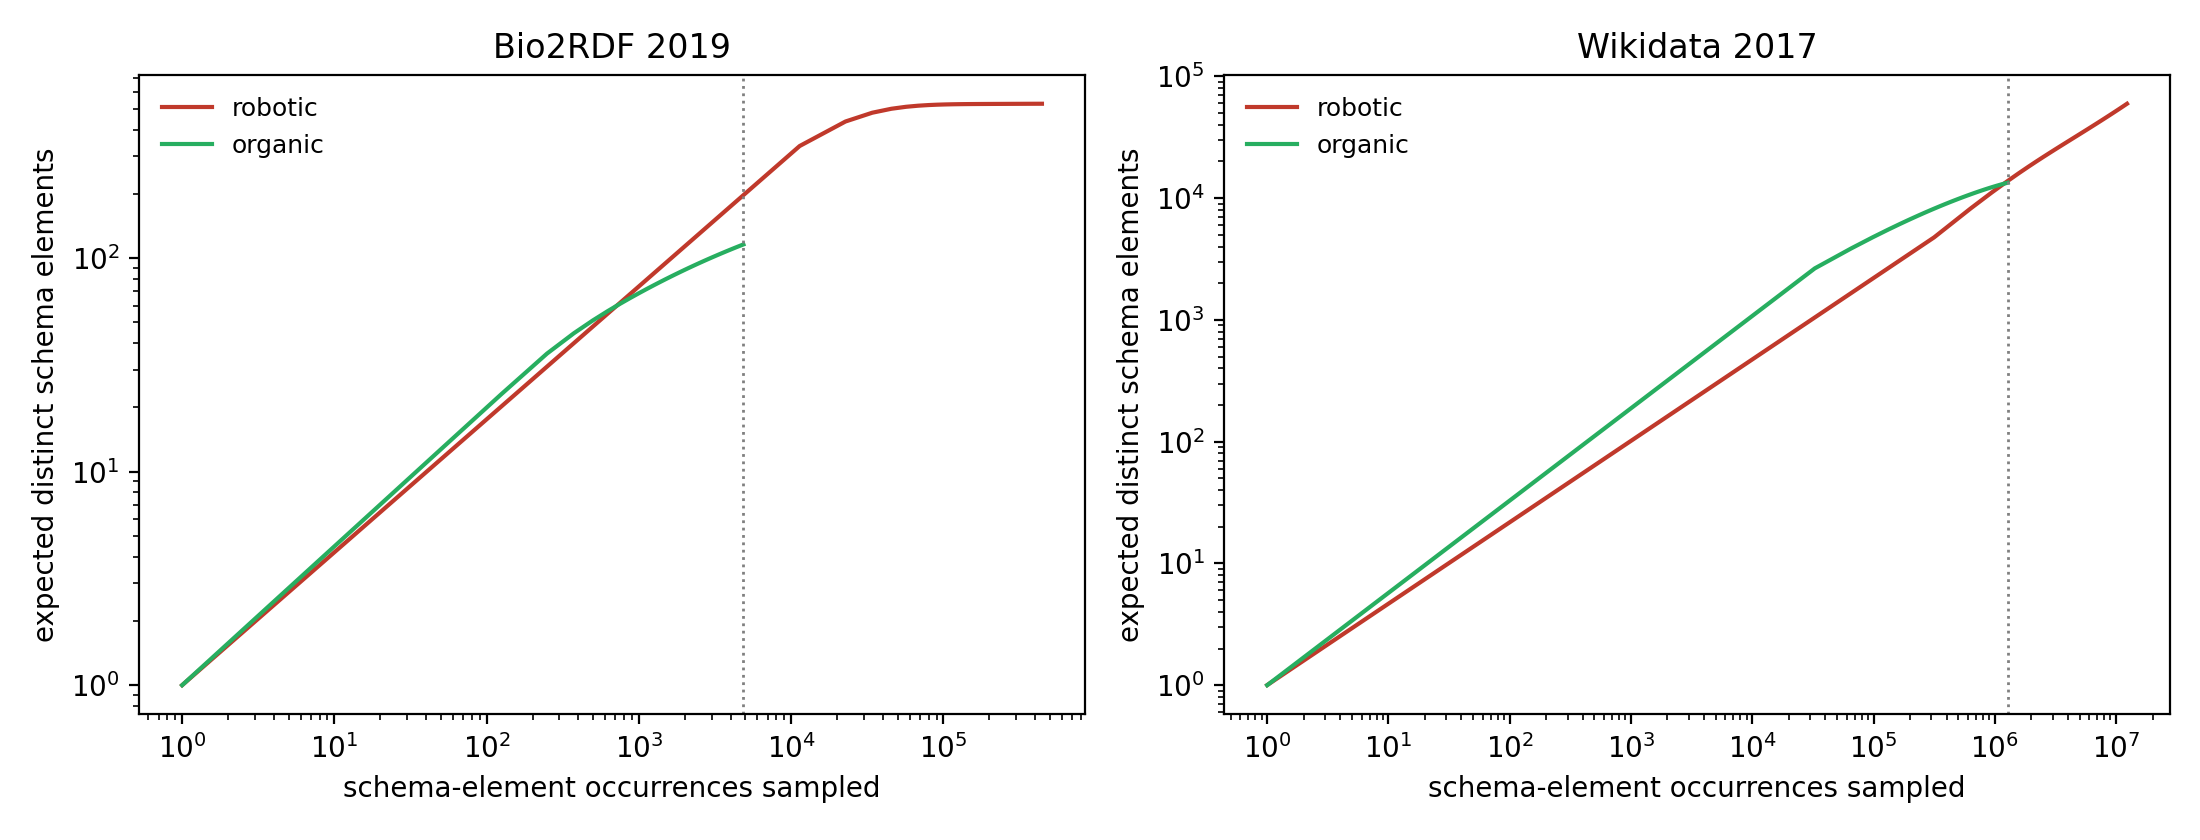
\includegraphics[width=0.95\textwidth]{rarefaction.png}
    \caption{Individual-based rarefaction curves (expected distinct schema elements vs.\ schema-element occurrences sampled, both axes log-scaled) for organic (green) and robotic (red) logs. The dotted line marks the maximum common sampling effort for the organic and robotic logs, corresponding to the size of the organic log. \DIFdelbeginFL \DIFdelFL{For Bio2RDF, }\DIFdelendFL \DIFaddbeginFL \DIFaddFL{In both KGs }\DIFaddendFL the \DIFdelbeginFL \DIFdelFL{robotic curve lies above }\DIFdelendFL \DIFaddbeginFL \DIFaddFL{two curves stay close over }\DIFaddendFL the \DIFdelbeginFL \DIFdelFL{organic curve across the }\DIFdelendFL shared sampling range\DIFdelbeginFL \DIFdelFL{; for Wikidata}\DIFdelendFL , \DIFdelbeginFL \DIFdelFL{the two curves are close, }\DIFdelendFL with organic queries showing \DIFaddbeginFL \DIFaddFL{slightly }\DIFaddendFL greater richness per occurrence at \DIFdelbeginFL \DIFdelFL{lower sampling efforts}\DIFdelendFL \DIFaddbeginFL \DIFaddFL{the common effort}\DIFaddendFL .}
    \label{fig:rarefaction}
\end{figure}

\begin{table}[ht]
\centering
\caption{Schema coverage at equal sampling effort. Robotic logs are rarefied down to the number of schema-element occurrences observed in the corresponding organic log.}
\label{tab:rarefaction}
\DIFdelbeginFL %DIFDELCMD < \begin{tabular}{l|r|r}
%DIFDELCMD < \hline
%DIFDELCMD < Comparison (equal effort) & Organic distinct elements (coverage) & Robotic distinct elements, rarefied (coverage) \\
%DIFDELCMD < \hline
%DIFDELCMD < Bio2RDF 2019 ($n=4{,}855$ occ.) & 116 (21.3\%) & $\approx$208 (38.2\%) \\
%DIFDELCMD < Wikidata 2017 ($n=1{,}279{,}731$ occ.) & 13,394 (12.8\%) & $\approx$13,846 (13.3\%) \\
%DIFDELCMD < \hline
%DIFDELCMD < \end{tabular}
%DIFDELCMD < %%%
\DIFdelendFL \DIFaddbeginFL \begin{tabular}{l|r|r}
\hline
Comparison (equal effort) & Organic distinct elements (coverage) & Robotic distinct elements, rarefied (coverage) \\
\hline
Bio2RDF 2019 ($n=1{,}220$ occ.) & 113 (20.9\%) & $\approx$99 (18.4\%) \\
Wikidata 2017 ($n=1{,}279{,}731$ occ.) & 13,394 (12.8\%) & $\approx$13,846 (13.3\%) \\
\hline
\end{tabular}
\DIFaddendFL \end{table}

Controlling for sampling effort \DIFdelbegin \DIFdel{produces markedly different results for the two }\DIFdelend \DIFaddbegin \DIFadd{removes the apparent robotic advantage in both }\DIFaddend KGs. For \textbf{Bio2RDF}, at the maximum common sampling effort \DIFdelbegin \DIFdel{, }\DIFdelend the robotic log recovers \DIFdelbegin \DIFdel{roughly $1.8\times$ }\DIFdelend \DIFaddbegin \emph{\DIFadd{no}} \DIFaddend more distinct schema elements than the organic log (\DIFdelbegin \DIFdel{208 }\DIFdelend \DIFaddbegin \DIFadd{99 }\DIFaddend vs.\ \DIFdelbegin \DIFdel{116; 38.2}\DIFdelend \DIFaddbegin \DIFadd{113; 18.4}\DIFaddend \% vs.\ \DIFdelbegin \DIFdel{21.3\%), and its rarefaction curve saturates near the full schema}\DIFdelend \DIFaddbegin \DIFadd{20.9\%)}\DIFaddend . A Monte-Carlo subsampling bootstrap (400 replicates, robotic rarefied to the organic effort of \DIFdelbegin \DIFdel{4}\DIFdelend \DIFaddbegin \DIFadd{1}\DIFaddend {,}\DIFdelbegin \DIFdel{855 }\DIFdelend \DIFaddbegin \DIFadd{220 }\DIFaddend occurrences) puts \DIFdelbegin \DIFdel{this }\DIFdelend \DIFaddbegin \DIFadd{the }\DIFaddend equal-effort ratio at \textbf{\DIFdelbegin \DIFdel{1.79}\DIFdelend \DIFaddbegin \DIFadd{0.88}\DIFaddend $\times$, 95\% CI [\DIFdelbegin \DIFdel{1.62}\DIFdelend \DIFaddbegin \DIFadd{0.75}\DIFaddend , \DIFdelbegin \DIFdel{1.96}\DIFdelend \DIFaddbegin \DIFadd{1.02}\DIFaddend ]}, \DIFdelbegin \DIFdel{comfortably above }\DIFdelend \DIFaddbegin \DIFadd{an interval that contains~}\DIFaddend 1\DIFdelbegin \DIFdel{, so robotic clients genuinely exercise a broader part of this small, specialized schema, consistent with automated enumeration or dumping}\DIFdelend \DIFaddbegin \DIFadd{: the two query types reach comparable breadth once effort is equalized, and the large raw gap in Table~\ref{tab:5} (97\% vs.\ 21\%) is a volume effect}\DIFaddend . For \textbf{Wikidata}, the picture reverses: at the maximum common sampling effort, the same bootstrap gives a ratio of only \textbf{1.03$\times$, 95\% CI [1.02, 1.05]} (robotic 13.3\% vs.\ organic 12.8\% of TSE), and at \emph{lower} effort organic queries are actually richer per occurrence (Figure~\ref{fig:rarefaction}, right). The raw coverage gap in Table~\ref{tab:5} (57\% vs.\ 13\%, i.e.\ $4.4\times$) therefore collapses to a $\sim$3\% difference once effort is equalized, which is consistent with that gap being largely attributable to robotic logs being two orders of magnitude larger rather than to broader robotic interest. (With $n\,{=}\,1.28$M the tiny residual is statistically distinguishable from 1.0, but its magnitude, 3\% vs.\ Bio2RDF's 79\%, is negligible.)

This size dependence is reinforced by how concentrated each log is on once-seen elements (Table~\ref{tab:singletons}). Two thirds of the schema elements counted for \emph{Wikidata-robotic-2017} are used exactly once; removing these singletons (the elements most exposed to one-off or erroneous uses) drops its coverage from 57.1\% to 18.9\% and shrinks the robotic-to-organic coverage ratio from $4.4\times$ to $2.0\times$. By contrast, \emph{Bio2RDF-robotic-2019} has a single singleton: its breadth is exercised repeatedly and is robust. In practical terms, for the two logs analysed here, robotic ``coverage'' on Wikidata largely reflects query volume and a long tail of one-off references, whereas on Bio2RDF it reflects systematic, repeated traversal of the schema. 



\begin{table}[ht]
\centering
\caption{Singleton sensitivity. Schema elements used exactly once, and coverage with vs.\ without singletons (2017 logs for Wikidata, 2019 for Bio2RDF).}
\label{tab:singletons}
\DIFdelbeginFL %DIFDELCMD < \begin{tabular}{l|r|r|r|r}
%DIFDELCMD < \hline
%DIFDELCMD < Log & Used elements & Singletons (\%) & Coverage & Coverage w/o singletons \\
%DIFDELCMD < \hline
%DIFDELCMD < Wikidata robotic & 59,603 & 39,900 (67\%) & 57.1\% & 18.9\% \\
%DIFDELCMD < Wikidata organic (full) & 13,394 & 3,412 (25\%) & 12.8\% & 9.6\% \\
%DIFDELCMD < Bio2RDF robotic & 529 & 1 (0.2\%) & 97.1\% & 96.9\% \\
%DIFDELCMD < Bio2RDF organic & 116 & 32 (28\%) & 21.3\% & 15.4\% \\
%DIFDELCMD < \hline
%DIFDELCMD < \end{tabular}
%DIFDELCMD < %%%
\DIFdelendFL \DIFaddbeginFL \begin{tabular}{l|r|r|r|r}
\hline
Log & Used elements & Singletons (\%) & Coverage & Coverage w/o singletons \\
\hline
Wikidata robotic & 59,603 & 39,900 (67\%) & 57.1\% & 18.9\% \\
Wikidata organic (full) & 13,394 & 3,412 (25\%) & 12.8\% & 9.6\% \\
Bio2RDF robotic & 525 & 1 (0.2\%) & 97.0\% & 96.9\% \\
Bio2RDF organic & 113 & 32 (28\%) & 20.9\% & 15.0\% \\
\hline
\end{tabular}
\DIFaddendFL \end{table}

\subsection{Bio2RDF-specific Analyses}\label{sec:bio2rdfresults}
Having established the general coverage metric (Section~\ref{s4}.5) and the equal-effort comparison (Section~\ref{sec:rarefaction}), we now group the analyses that apply only to Bio2RDF: what its organic log actually contains, the recovery of an organic/robotic split for the 2013 era, and the effect of matching the schema to the release each log actually queried.

\paragraph{\textbf{What the Bio2RDF organic-2019 log actually contains.}} The organic/robotic split (Section~\ref{s2}) is a user-agent proxy, and a browser user agent does not guarantee a human information need. Inspecting the 8{,}140 valid unique organic-2019 queries shows that \textbf{86.9\% reference no Bio2RDF schema element at all}: they are the endpoint's default-sample query (\texttt{select * where \{[] a ?Concept\} LIMIT 100}), liveness checks (\texttt{select ?s where \{?s ?p ?o\} limit 1}), Virtuoso-internal test queries with \texttt{OPTION(RVR/BREAKUP)} against \texttt{no-such-*} IRIs, and bare label/dereference lookups, automated or non-informative browser traffic rather than human information-seeking, the 2019 counterpart of the infrastructure contamination we document for the raw 2013 log (Section~\ref{sec:bio2013}, Table~\ref{tab:bio2013comp}). Only \textbf{1{,}065 queries (13.1\%) are schema-bearing}, and it is these that produce the \DIFdelbegin \DIFdel{116 }\DIFdelend \DIFaddbegin \DIFadd{113 }\DIFaddend used elements and the \DIFdelbegin \DIFdel{21.3}\DIFdelend \DIFaddbegin \DIFadd{20.9}\DIFaddend \% organic coverage. This does not inflate coverage or concentration, schema-less queries contribute \emph{zero} used elements, so the numerator is drawn entirely from the schema-bearing minority, but it does mean the Bio2RDF organic-2019 figures characterise a small core of genuine human queries, not the raw browser stream, and any organic/robotic behavioural contrast on Bio2RDF-2019 should be read with that in mind. We therefore restrict the query-template analysis (Section~\ref{sec:templates}) to schema-bearing queries.

\subsubsection{Organic vs.\ Robotic in the 2013-era Bio2RDF Log}\label{sec:bio2013}
The LSQ-derived \emph{Bio2RDF-all-2013} log is anonymized and cannot be split by user agent. To examine the 2013 era at the same organic/robotic granularity as the rest of the paper, we processed the \emph{raw} Bio2RDF server access log (the upstream source of LSQ), spanning May 2013--September 2015. It contains 127.2M executed SPARQL requests (HTTP~200), each carrying a user agent and the dataset endpoint (\texttt{cu.\textit{dataset}.bio2rdf.org}).

The first lesson is about what such a log actually contains (Table~\ref{tab:bio2013comp}): \textbf{organic (browser) queries are only 0.09\%} of executed traffic. The bulk is machine-generated and, revealingly, much of it is \emph{infrastructure}: 24\% are Bio2RDF's own Virtuoso engine acting as an HTTP client (federated \texttt{SERVICE} calls and dereferencing, 99.6\% of these come from a single host in the hosting institution's network, and their bodies are single-entity label/cross-reference lookups), and a further 22\% is a sustained empty-user-agent crawl from the network of the LSQ project itself, i.e.\ the harvesting that built the public dataset. Any usage statistic computed over the raw log without removing such traffic would largely measure the infrastructure rather than users, a concrete instance of the example-/tool-contamination concern that any log study must control for.

\begin{table}[ht]
\centering
\caption{Composition of the raw 2013--2015 Bio2RDF server log (127.2M executed SPARQL requests) by user-agent class. Genuine human (browser) traffic is 0.09\%; about half of all traffic is the endpoint's own Virtuoso federation/dereferencing or the LSQ harvest.}
\label{tab:bio2013comp}
\begin{tabular}{l|r}
\hline
User-agent class & Share of executed requests \\
\hline
Programmatic tools / libraries (Java, Jena, \ldots) & 49.8\% \\
Virtuoso-internal (federation / dereferencing) & 24.4\% \\
LSQ-harvest (sustained empty-UA crawl) & 22.4\% \\
Search-engine crawlers & 1.7\% \\
Other / no agent & 1.6\% \\
\textbf{Organic (browser)} & \textbf{0.09\% (115{,}420)} \\
\hline
\end{tabular}
\end{table}

Restricting to the 115{,}420 organic queries (61{,}628 unique; 50.3\% syntactically valid, the rest is the non-SPARQL web spam noted in Section~\ref{s4}.3), 2013-era organic queries cover \textbf{\DIFdelbegin \DIFdel{53.6}\DIFdelend \DIFaddbegin \DIFadd{53.4}\DIFaddend \% of the 2024 Bio2RDF schema} (167/350 types, \DIFdelbegin \DIFdel{125/195 }\DIFdelend \DIFaddbegin \DIFadd{122/191 }\DIFaddend predicates), exercising the expected biomedical core (\emph{drugbank:Drug}, \emph{omim:Gene}/\emph{Phenotype}, \emph{drugbank:Target}, \emph{kegg:Pathway}, \emph{pharmgkb:Disease}). This is far above the \DIFdelbegin \DIFdel{21.3}\DIFdelend \DIFaddbegin \DIFadd{20.9}\DIFaddend \% of organic-2019, but the comparison must control for effort: the 2013 organic log has roughly five times as many unique queries. Rarefying both to equal sampling effort (Section~\ref{sec:rarefaction}), organic-2013 recovers \DIFdelbegin \DIFdel{33.7}\DIFdelend \DIFaddbegin \DIFadd{26.7}\DIFaddend \% vs.\ organic-2019's \DIFdelbegin \DIFdel{21.3}\DIFdelend \DIFaddbegin \DIFadd{20.9}\DIFaddend \%, a residual \textbf{\DIFdelbegin \DIFdel{1.58}\DIFdelend \DIFaddbegin \DIFadd{1.28}\DIFaddend $\times$} difference that persists after controlling for sampling effort. One possible explanation is architectural: in 2013 Bio2RDF exposed a \emph{separate endpoint per dataset}, so human exploration may have spread across the specialized subgraphs, whereas the single unified 2019 endpoint may have concentrated organic queries on a narrower core. We cannot test this directly, since the endpoint architecture and the six-year time gap change together.

This analysis contributes two things. First, it supplies the organic/robotic split for the 2013 era, which the anonymized LSQ release does not permit. Second, it adds a temporal comparison of organic coverage within Bio2RDF. Both reinforce the methodological point of Section~\ref{sec:rarefaction}: raw coverage is strongly affected by sampling effort, so equal-effort comparisons provide a fairer basis for comparing schema coverage.

\paragraph{\textbf{Schema-version robustness.}} The coverage above is measured against the 2024 endpoint schema, but the queries hit \emph{earlier} Bio2RDF releases, and the schema evolved substantially across them. The 2019 log queried the same release (Release~4) that the 2024 endpoint still serves, so it is already version-matched. The 2013 log is the problem: only \textbf{17.5\% of the vocabulary IRIs it references appear in the 2024 schema}, because datasets were retired and per-dataset vocabularies revised across releases (38 of the 59 datasets queried in 2013 are absent from the 2024 endpoint). Moreover, the raw 2013--2015 organic log \emph{straddles two releases}: Release~2 (2012--2013 data) until Release~3 was deployed in mid-2014 (Release~3 grew the corpus from 25 to 35 datasets, e.g.\ adding \emph{chembl}, \emph{sider}, \emph{reactome}).

We therefore recovered both schemas from Bio2RDF's published per-dataset statistics files (Release~2: 157 types, 628 predicates; Release~3: 351 types, 1{,}744 predicates), split the organic log at the mid-2014 boundary (35.8K queries before, 80.5K after), and matched each part to the release it actually queried. Version alignment recovers most of the apparently ``missing'' vocabulary: the fraction of referenced vocabulary present in the schema rises from 17.5\% (against 2024) to \textbf{48\%} for the Release-2 period (against Release~2) and \textbf{62\%} for the Release-3 period (against Release~3). The corresponding version-matched coverage is 53\% (417/782) and 36\% (761/2{,}095).

The historical schemas and the 2024 schema are obtained differently. Our 2024 denominator is obtained by querying a live endpoint, which lets us apply the restrictive definition of Section~\ref{s3}.2 (vocabulary types excluding \texttt{}, and only those predicates that connect two vocabulary types). Releases~2 and~3 are no longer served by any endpoint, so the only surviving record of their schemas is Bio2RDF's published per-dataset statistics files, which enumerate all predicates and only instantiated types. Because we cannot re-derive the restrictive definition from those files, the historical denominators are on a broader basis than the 2024 one. Therefore, the version-matched coverage values are not directly comparable to each other or to our headline figures. Ideally, the same schema definition would be applied to every release, but this is not possible because of this data-availability constraint.

The direction of the resulting bias is nevertheless known: a broader denominator can only \emph{lower} the version-matched percentages, so it cannot manufacture the increase we report. The robust, directional conclusion is that the 2024 schema substantially underestimates historical vocabulary, so the 2024-based 2013 coverage is a conservative cross-version estimate; aligning the schema to the queried release raises, not lowers, it. We retain the 2024-schema figures in Tables~\ref{tab:4} and~\ref{tab:5} and treat the version-matched recomputation as a robustness check; the recovered Release-2 and Release-3 schemas are released with our artifacts.

\begin{figure}
    \centering
    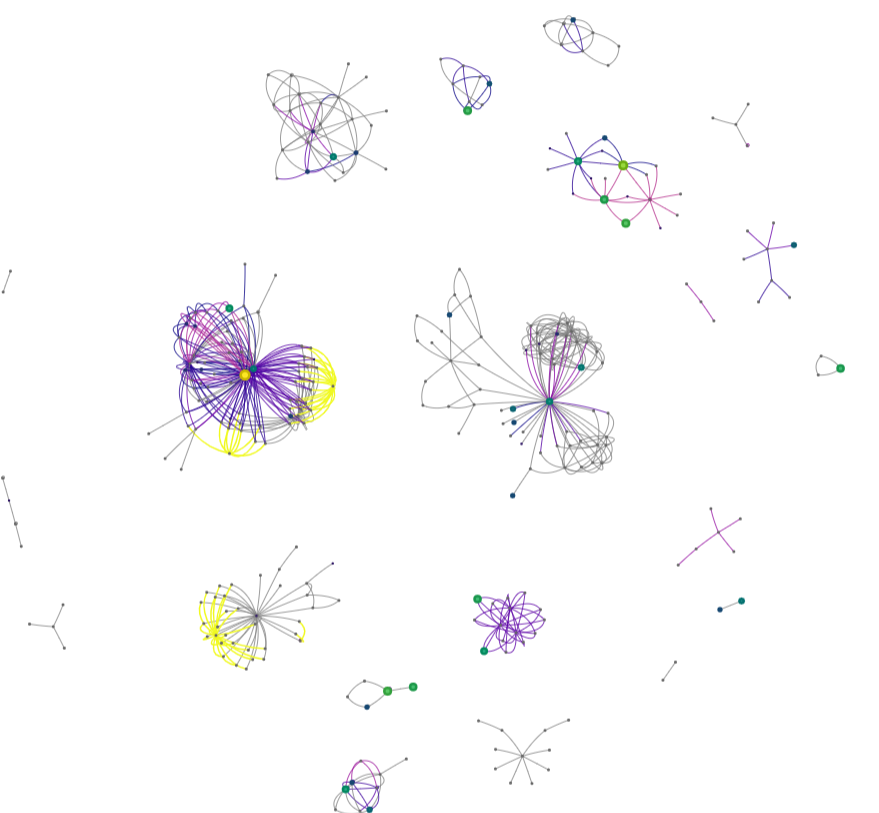
\includegraphics[width=0.6\textwidth]{image21.png} 
    \caption{Visualization of schema-element usage in \emph{Bio2RDF-organic-2019} (KG2024). Node size and color both increase with usage frequency (small/dark = rarely used, large/bright = heavily used); edge width increases with predicate usage; schema elements not used in any query are gray. The few large, bright hubs concentrate most of the usage.}
    \label{fig:l5}
\end{figure}

Figure \ref{fig:l5} illustrates the extent to which schema elements of the Bio2RDF KG are used in the organic queries of 2019. Nodes represent schema types and edges represent predicates linking instances of those types. Both the size and the color of a node encode the same quantity, its usage frequency: nodes grow larger and brighter as they are queried more often, while rarely used nodes are small and dark. Edge width likewise grows with predicate usage, and schema elements that appear in no query are shown in gray. The visualization makes the long tail visible directly: a handful of large, bright hubs (drug, gene, and disease types) concentrate the bulk of organic usage, while most of the schema remains gray and unqueried. The interactive version, with exact per-element values, is available online\footnote{\url{https://marmhm.github.io/Schema-usage-graph/}}.


\subsubsection{Pairwise Schema Type Usage of Bio2RDF}\label{sec:pairwise}

Bio2RDF is organized into 26 interconnected subgraphs corresponding to different source datasets, each with its own vocabulary. This structure allows us to examine how queries connect elements from different Bio2RDF subgraphs. We therefore perform this analysis only for Bio2RDF, as it relies specifically on its subgraph organization. For each triple pattern in a SPARQL query, we identify the subgraphs associated with its subject and object and record a cross-subgraph pair when they belong to two different subgraphs. We use these pairs to examine how frequently different Bio2RDF subgraphs are connected in queries and how this usage changes over time.

What we measure is the \emph{pairwise schema type pattern}: a query triple that links a type from one subgraph to a type from another via a (typically variable) predicate, i.e.\ an attempt to join data across datasets. We count how many \emph{distinct} such subgraph pairs appear in each log, comparing 2013 (log\_2013, covering 17 subgraphs) and 2019 (log\_2019, covering 26 subgraphs), following the procedure of Section~\ref{sec:s62}.

The number of distinct cross-subgraph join patterns observed in queries rose from \textbf{3 in log\_2013 to 22 in log\_2019}, roughly a sevenfold increase. These two values are the counts of non-zero cells in the two heatmaps of Figure~\ref{fig:l7}: each non-zero cell is one observed subgraph pair, so the 2013 panel has three populated cells and the 2019 panel twenty-two. We report this as a count rather than a fraction of ``possible'' patterns: the space of possible cross-subgraph joins is large (the schema exhibits 430 directed cross-subgraph type-to-type edges across 26 subgraphs) and, because observed joins use variable predicates rather than specific schema edges, a ``used-out-of-possible'' ratio would compare two different notions. The robust and reproducible quantity is the increase in distinct observed join patterns.

Figure \ref{fig:l7} presents a heatmap illustrating the pairwise schema type usage across Bio2RDF subgraphs for log\_2013 and log\_2019. The results highlight a significant increase in the diversity of dataset integration in 2019 relative to 2013. This shift reflects broader advancements in data accessibility and integration practices within the bioinformatics community. The observed increase is likely attributable to the adoption of a single query endpoint for all datasets in 2019, which improved accessibility compared to the multiple endpoints used in 2013.

\begin{figure}
    \centering
    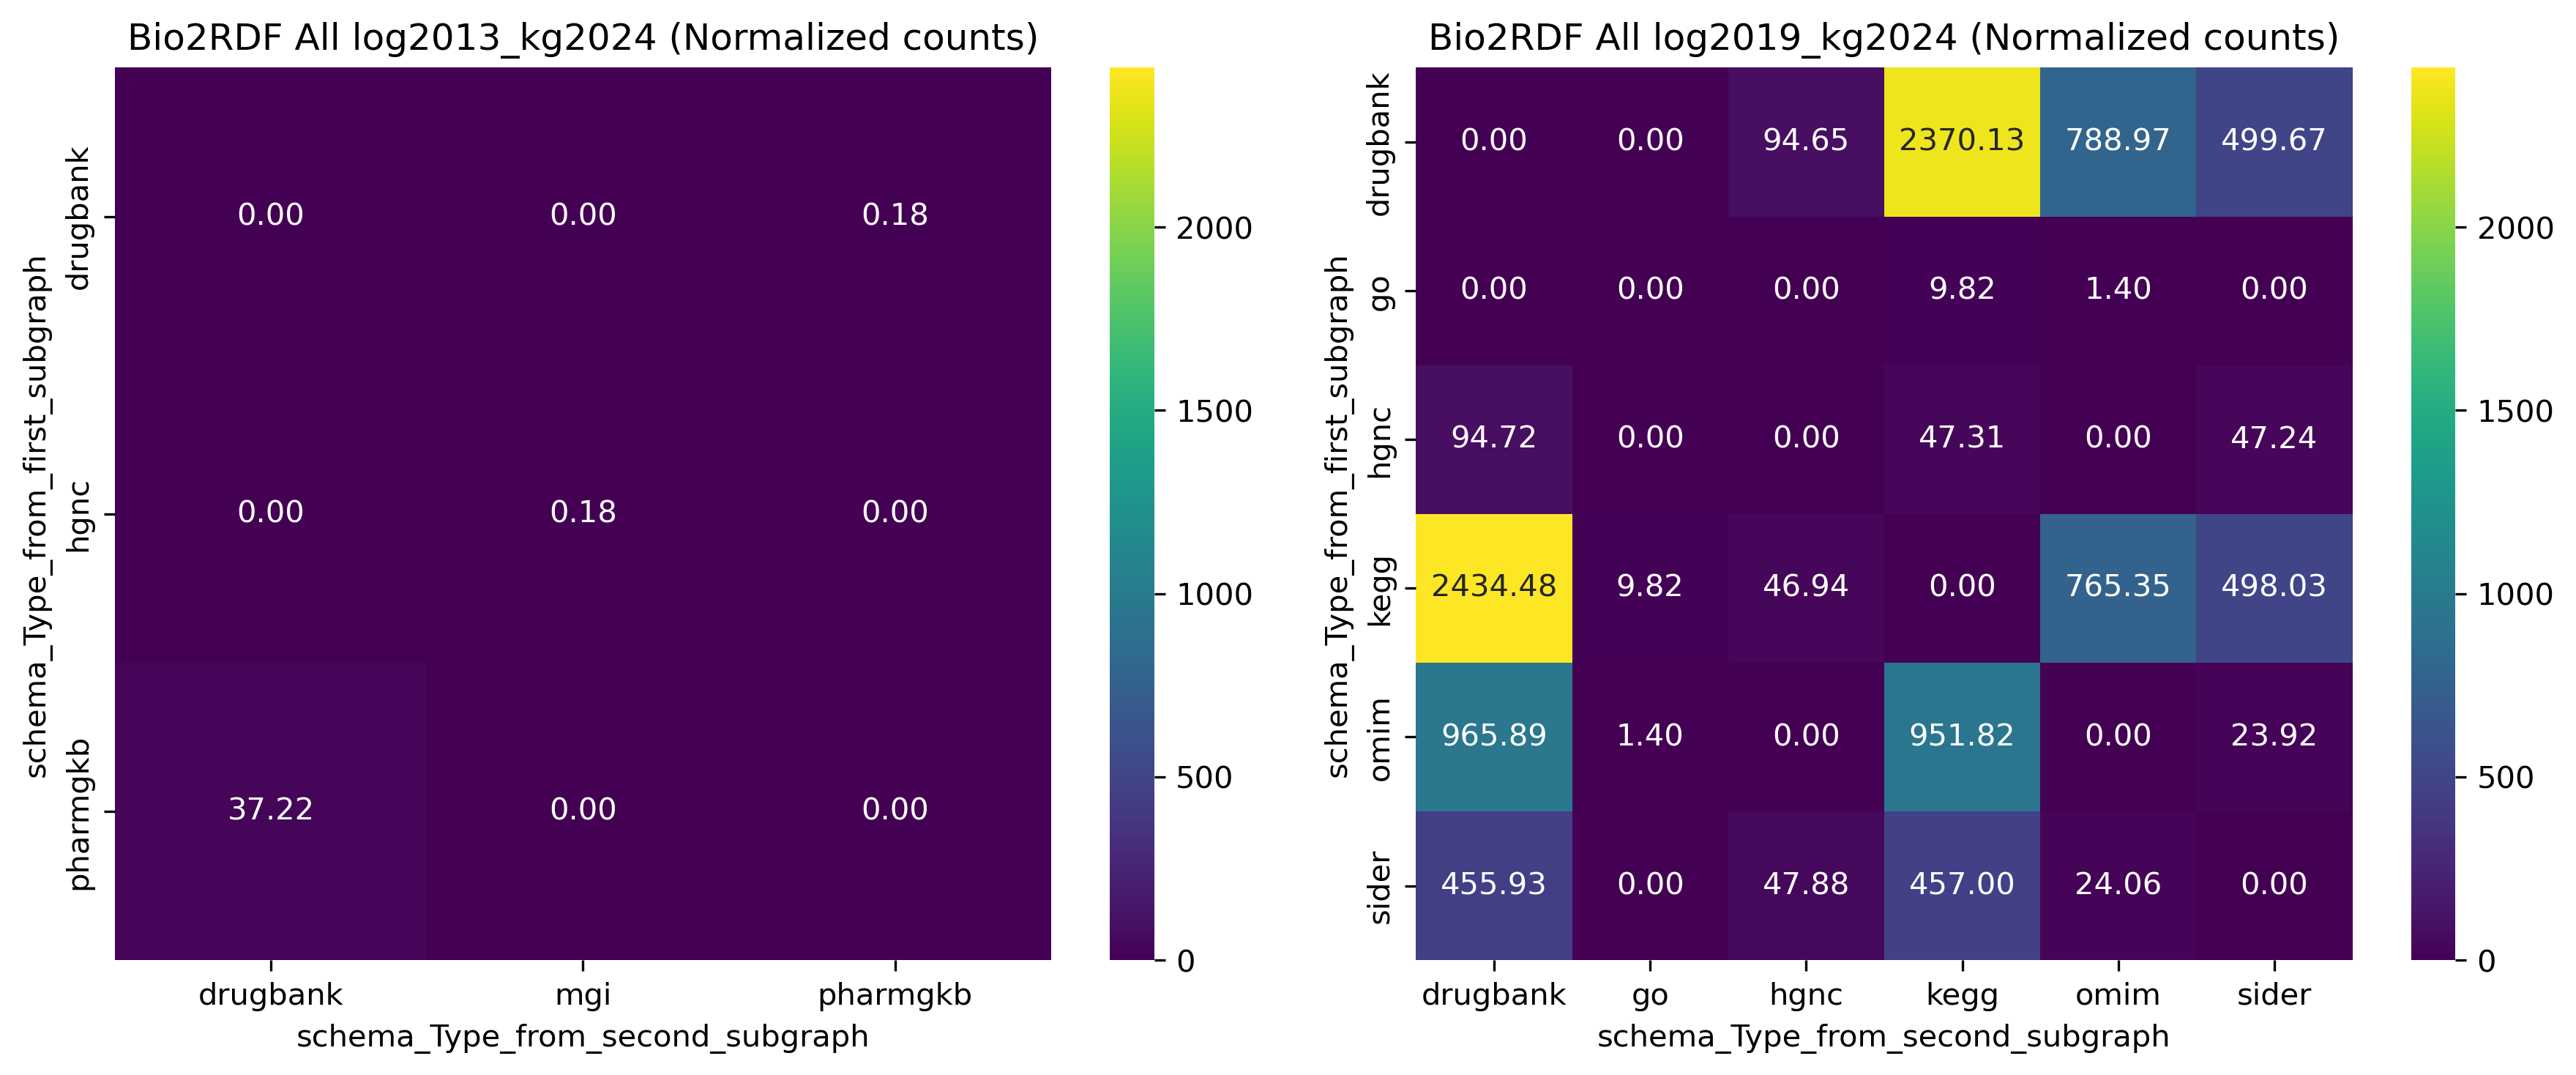
\includegraphics[width=0.8\textwidth]{image24.png} 
    \caption{Heatmap of the pairwise co-occurrence of schema types from two different subgraphs of log 2013 vs. 2019
}
     \label{fig:l7}
\end{figure}

\subsection{Wikidata-specific Analyses}\label{sec:wdresults}
We now turn to the analyses specific to Wikidata, whose item-based model raises measurement questions that do not arise for Bio2RDF: whether the entities we extract as classes are genuine schema, and whether they are referenced as classes at all.

\paragraph{\textbf{Validity of the extracted classes.}} Because a Wikidata ``class'' is just an item used as the object of \texttt{wdt:P31}/\texttt{wdt:P279}, one must ask how many extracted classes are genuine schema rather than uninstantiated or one-off (possibly erroneous) edits. We characterize each class by its \emph{support}: the number of times it is the object of \texttt{wdt:P31} or \texttt{wdt:P279} in the KG (instances plus subclasses). Of the 103{,}355 extracted 2017 classes, 42.3\% are instantiated ($\geq 1$ instance), 88.2\% are embedded in the subclass hierarchy, and 30.3\% are \emph{singletons} (used as a class exactly once), the elements most exposed to data glitches. Crucially, \emph{querying selects for well-supported classes}: among the classes referenced in organic-2017 queries, 72.5\% are instantiated (vs.\ 42.3\% of all extracted 2017 classes), the median support is 9 (vs.\ 3), and only 15.8\% are singletons. To check whether even the singleton tail is spurious, we drew a random sample of 100 queried singletons and looked them up. Of these, 80\% carry an explicit \texttt{wdt:P279} (\emph{subclass of}) statement or a metaclass marker, meaning they were intentionally modelled as classes. Manual inspection of the remainder finds mostly genuine but rarely used concepts rather than errors: some are biological taxa (e.g.\ \emph{Quercus velutina}, \emph{Pinales}), others are specialised non-taxonomic concepts (e.g.\ \emph{ghat}, a South Asian riverside step structure). Outright noise, such as a disambiguation item, is rare. Thus, data-quality issues may slightly affect the metric, but the effect appears limited and is concentrated among rare, uninstantiated classes that are seldom queried.

\subsubsection{What Wikidata Coverage Actually Measures: Class- vs.\ Value-Position Usage}\label{sec:classvalue}
A schema-coverage metric assumes that the elements it counts are referenced as classes or predicates, rather than appearing as data values. Bio2RDF vocabulary classes are only ever referenced as classes, so the assumption holds there. Wikidata items, by contrast, frequently appear both as classes and as values: the same item is routinely referenced as the value of a property (e.g.\ \texttt{Q33999} \emph{actor} as the value of \texttt{P106} \emph{occupation}) rather than as a class. We therefore re-examine the Wikidata results by classifying every entity reference as class-position (object of \texttt{wdt:P31}/\texttt{wdt:P279}, or of a path involving them) or value-position (Section~\ref{s3}.2).

Table~\ref{tab:classvalue} shows the split. Among the entities our extraction counts as Wikidata \emph{used types} (those referenced in queries that are also objects of \texttt{wdt:P31}/\texttt{wdt:P279} in the KG), only \textbf{70.2\% of organic} ones are ever used as a class, \textbf{29.8\% are referenced solely as values}, whereas robotic queries use 92.9\% of their counted types as classes. \DIFdelbegin \DIFdel{Weighted }\DIFdelend \DIFaddbegin \DIFadd{Weighting }\DIFaddend by reference volume \DIFdelbegin \DIFdel{the contrast narrows (both query types are dominated by value references , since queries fetch values): only $\sim$27--29\% of all type-item references are in class position.
}\DIFdelend \DIFaddbegin \DIFadd{rather than by distinct element does not narrow this contrast; it inverts it, and the inversion is the more informative result. Counting references rather than elements, }\textbf{\DIFadd{90.7\% of organic type-item references are in class position}} \DIFadd{(2.78M of 3.07M) against }\textbf{\DIFadd{61.3\% of robotic ones}} \DIFadd{(6.24M of 10.19M). So on the set-level view robotic queries look the more class-oriented of the two (92.9\% vs 70.2\%), while on the volume-weighted view organic queries do (90.7\% vs 61.3\%).
}

\DIFadd{Both views are correct and they measure different things. For organic queries the value-only items are numerous but individually rare: they are 29.8\% of the distinct type-items a human touches yet draw under a tenth of the references to type-items. Human value-position usage is thus a long tail of one-off mentions. Robotic traffic shows the opposite profile: few distinct type-items are value-only (7.1\%), but those that are get referenced in enormous volume, so nearly two fifths of robotic type-item references sit in value position.
}

\DIFadd{This matters for how the over-counting should be understood. Because coverage is a breadth measure (Section~\ref{sec:concentration}), it is the }\emph{\DIFadd{set-level}} \DIFadd{figure that determines how much a coverage percentage is inflated, and that inflation is worst for human queries. The volume-weighted figures do not correct the coverage metric; they show that the two query types arrive at their schema usage by different routes, which the single set-level contrast conceals. }\DIFaddend These results have two implications. First, the published Wikidata coverage \emph{over-counts schema usage}, most so for human queries, where roughly a third of the ``used types'' are mis-counted value-items (\emph{actor}, \emph{female}, \emph{India}). Second, the class/value split differs systematically between the two query types in these logs\DIFdelbegin \DIFdel{: organic queries reference }\DIFdelend \DIFaddbegin \DIFadd{, though the direction depends on whether one counts elements or references: a larger }\emph{\DIFadd{share of the distinct type-items}} \DIFadd{organic queries touch is value-only (29.8\% vs 7.1\%), whereas a larger }\emph{\DIFadd{share of the references}} \DIFadd{robotic queries make to }\DIFaddend type-items \DIFdelbegin \DIFdel{as values far more often than robotic ones, which reference them in class position}\DIFdelend \DIFaddbegin \DIFadd{is value-position (38.7\% vs 9.3\%). We report this as a difference between the analysed logs; establishing that it reflects querying behavior in general, rather than characteristics of this particular sample of clients and time period, would require further evidence}\DIFaddend . 


\begin{table}[ht]
\centering
\caption{Class- vs.\ value-position usage of the Wikidata ``used types'' (2017). A type is used \emph{as a class} only when it is the object of \texttt{wdt:P31}/\texttt{wdt:P279} (or a path involving them) in a query.}
\label{tab:classvalue}
\begin{tabular}{l|r|r|r}
\hline
Query type & \#Used types & Used as a class & Value-only \\
\hline
Wikidata organic 2017 & 12,773 & 8,968 (70.2\%) & 3,805 (29.8\%) \\
Wikidata robotic 2017 & 58,689 & 54,534 (92.9\%) & 4,155 (7.1\%) \\
\hline
\end{tabular}
\end{table}

\DIFdelbegin \DIFdel{Beyond the position of reference, comparing query }\DIFdelend \DIFaddbegin \DIFadd{The position analysis above establishes that Wikidata's coverage figure over-counts, but it leaves a second question open, and the two together are what make the coverage number interpretable. Coverage asks how much of the schema is reached; it says nothing about whether the parts that are reached are the parts the KG is actually built around. If the heavily populated regions of the KG were also the heavily queried ones, a low coverage figure would simply mean users query a small but well-chosen core. We therefore compare query }\DIFaddend \emph{demand} against KG \emph{supply} (instances per class, extracted from the dump)\DIFdelbegin \DIFdel{reveals a }\DIFdelend \DIFaddbegin \DIFadd{.
}

\DIFadd{We run this comparison on Wikidata, and later on DBpedia, rather than on Bio2RDF, for a reason specific to what coverage looks like on each. A supply--demand inversion can only exist where a substantial part of the schema goes unqueried, and on Bio2RDF it does not: the union of 2019 queries reaches 97\% of the schema (Table~\ref{tab:5}), leaving 16 elements of 541 untouched. There is no appreciable body of Bio2RDF content that nobody queries, so the comparison would have nothing to find. On Wikidata, organic queries reach about 4\% of the class universe, which leaves the overwhelming majority of the KG's content unqueried and makes the question of }\emph{\DIFadd{which}} \DIFadd{content that is a substantive one.
}

\DIFadd{The answer is a }\DIFaddend pronounced inversion (Figure~\ref{fig:mismatch}). The most heavily instantiated Wikidata classes are almost never queried: e.g.\ \emph{ravine} ($\sim$17{,}000 instances), \emph{reef}, \emph{cairn}, \emph{qanat}, \emph{shoal}, and (for bots) \emph{Wikimedia navigational template} ($\sim$27{,}000), \emph{protein domain}, and \emph{microRNA}, all bulk- or bot-imported categories with essentially zero human or robotic class-position demand. Conversely, the genuinely class-queried core is small and intuitive: \emph{human} (\texttt{Q5}), \emph{city}, \emph{film}, \emph{country}, \emph{painting} for organic queries, and \emph{human-geographic territorial entity}, \emph{film}, \emph{album}, \emph{church building}, \emph{book}, \emph{business} for robotic. In other words, the bulk of what Wikidata \emph{contains} is not what users \emph{query}, and much of what users query as ``types'' the model does not treat as classes at all.
\DIFdelbegin %DIFDELCMD < \begin{comment}%DIFDELCMD < 
%DIFDELCMD <     the paragraph starting with "Beyond the position of reference...", I belive that the supply-demand analysis is introduced abruptly, with no relation to the schema coverage or wikidata specific analysis. why would we not calculated this supply-demnd analysis for Bio2RDf, I dont sugesst doing it, instead my question is in first place why did we do it for wikidata? in the current presentation it seems unrelevant and not justified. 
%DIFDELCMD < \end{comment}
%DIFDELCMD < %%%
\DIFdelend 

\begin{figure}
    \centering
    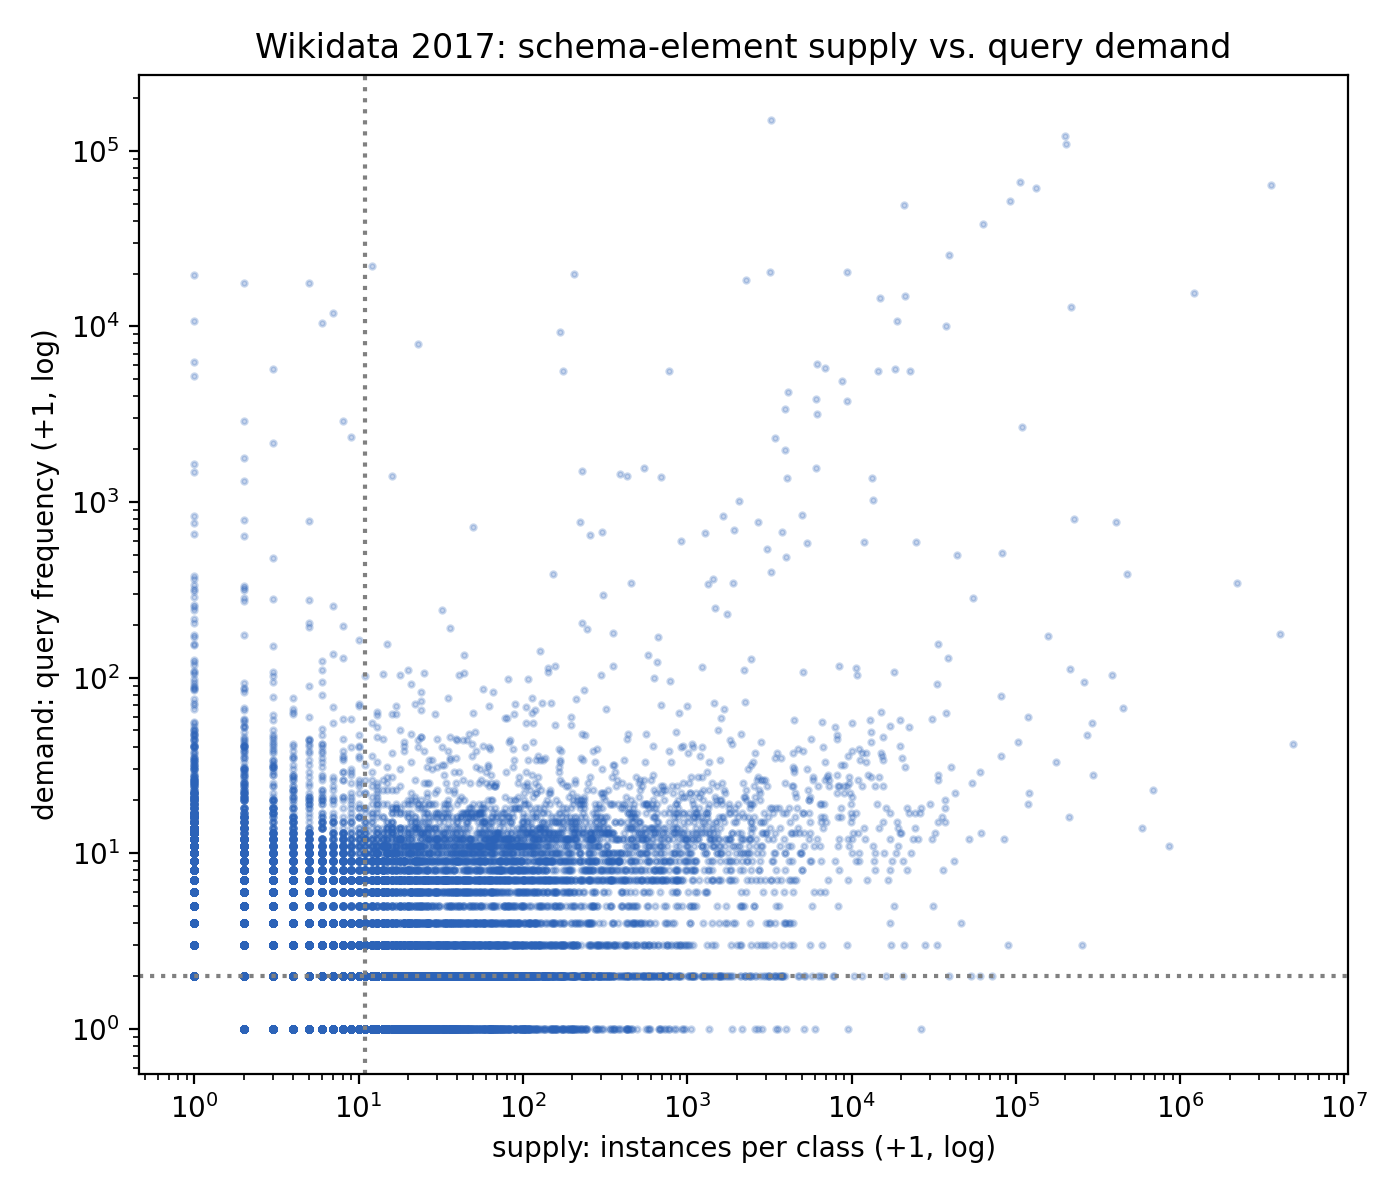
\includegraphics[width=0.6\textwidth]{wd_mismatch.png}
    \caption{Wikidata schema-element supply (instances per class, from the 2017 dump) vs.\ organic query demand (query frequency). Dotted lines mark the high-supply and high-demand thresholds. Heavily instantiated classes (lower right) attract little query demand, while the highest-demand items (upper left) have few or no instances because they are queried as values, not classes.}
    \label{fig:mismatch}
\end{figure}

The inversion is not confined to individual classes: a similar pattern is observed across the analyzed \emph{domains}. We assigned each class to a top-level domain by walking up its \texttt{wdt:P279} ancestry to a curated set of anchor classes, and compared each domain's share of KG content with its share of query demand (Table~\ref{tab:domains}).

Two points of interpretation are needed before reading that table. First, the ``supply'' column is a share of \emph{instances}, not of classes: it gives the proportion of all classified Wikidata items whose class falls in that domain. For example, \emph{taxon} accounts for 7.6\% of supply because 7.6\% of all classified items are instances of some class in the taxon domain, not because 7.6\% of classes are taxonomic. Second, the comparison is deliberately between instance-level supply and class-level demand: we count how often classes in a domain are referenced in queries, and compare that with how much data sits under those classes in the KG. The question it answers is whether users query classes in proportion to the amount of data available under them; it is not an instance-to-instance comparison, and a reader expecting one would misread the columns. The pattern is stark: the bulk-imported scientific and bibliographic domains: \emph{taxon}, \emph{gene/protein}, \emph{astronomical object}, and \emph{scholarly publication}, together hold \textbf{32\% of all instances but draw only $\sim$5\% of organic demand} (\emph{taxon} alone: 7.6\% of content, 0.4\% of demand). Conversely, the \emph{person} and \emph{organization} domains hold 15\% of content but attract \textbf{$\sim$39\% of organic demand}. The split also sharpens the organic/robotic contrast, and the two demand-to-supply ratio columns make it directly comparable: human queries concentrate on \emph{person} (29.8\%, ratio 2.48, vs.\ 14.4\% and 1.20 for bots), whereas robotic queries are far heavier on \emph{scholarly publication} (14.3\%, ratio 0.75, vs.\ 2.4\% and 0.13) and \emph{geographic features} (21.9\%, ratio 1.37, vs.\ 11.1\% and 0.69). Notably, \emph{geographic features} is the one domain that bots over-query relative to content while humans under-query it. This is consistent with automated bibliographic and gazetteer harvesting. (The residual ``Other'' bucket carries 17.9\% of organic demand and includes the value-position items of Section~\ref{sec:classvalue}, which have no clean class-domain.)

\begin{table}[ht]
\centering
\caption{Content--demand inversion by domain (Wikidata 2017). Each class is assigned to a top-level domain via its \texttt{wdt:P279} ancestry. ``Supply'' is the domain's share of KG content measured in \emph{instances} (the proportion of all classified items whose class lies in that domain), and ``Organic''/``Robotic'' are its shares of class-position query demand. Each demand share is accompanied by its ratio to the supply share ($<1$ = under-queried relative to content, $>1$ = over-queried); no ratio is given for the unclassified residual, whose supply share is not a meaningful denominator.}
\label{tab:domains}
\begin{tabular}{l|r|r|r|r|r}
\hline
Domain & Supply (\% instances) & Organic (\%) & Org/supply & Robotic (\%) & Rob/supply \\
\hline
Taxon / species              & 7.6\%  & 0.4\%  & 0.05 & 0.0\%  & 0.00 \\
Scholarly / publication      & 19.1\% & 2.4\%  & 0.13 & 14.3\% & 0.75 \\
Gene / protein / biomedical  & 4.9\%  & 1.9\%  & 0.39 & 1.7\%  & 0.35 \\
Astronomical object          & 0.5\%  & 0.3\%  & 0.60 & 0.1\%  & 0.20 \\
Creative work                & 33.1\% & 21.8\% & 0.66 & 23.3\% & 0.70 \\
Geographic feature           & 16.0\% & 11.1\% & 0.69 & 21.9\% & 1.37 \\
Person (human/occupation)    & 12.0\% & 29.8\% & 2.48 & 14.4\% & 1.20 \\
Organization / company       & 3.3\%  & 9.1\%  & 2.76 & 14.0\% & 4.24 \\
Event                        & 1.2\%  & 5.4\%  & 4.5  & 3.0\%  & 2.50 \\
Other / unclassified         & 2.2\%  & 17.9\% &, & 7.2\%  &, \\
\hline
\end{tabular}
\end{table}

\paragraph{\textbf{A third KG DBpedia.}} An alternative explanation is that the observed value-position usage is specific to Wikidata's modeling conventions, or to its size, rather than to the item-based modeling style as such. To test this we added a third KG, DBpedia, and ran the same class- vs.\ value-position analysis over its public query log (LSQ~2.0). DBpedia is a useful control: like Bio2RDF it is OWL-style: its classes are dedicated ontology IRIs (\texttt{dbo:}) used as the object of \texttt{rdf:type}/\texttt{rdfs:subClassOf}, but like Wikidata it is large, broad, and crowd-curated, so it separates the effect of \emph{schema model} from that of \emph{size and breadth}. Across 4.26M distinct executed queries, of the 722 \texttt{dbo:} classes referenced anywhere, \textbf{675 (93.5\%) are used in class position and only 47 (6.5\%) are value-only}, close to Bio2RDF's near-zero and far below Wikidata's 29.8\% for human queries (Table~\ref{tab:generality}). These results suggest that the value-only fraction is more closely associated with the data model than with KG size: across the three KGs analysed, the two OWL-style ones both keep classes in class position, whereas the item-based Wikidata routinely surfaces type-items as values. The content--demand inversion also recurs on DBpedia: its most heavily instantiated classes (\emph{Tenure}, $\sim$1.3M instances; \emph{WikimediaTemplate}, $\sim$223k; \emph{MilitaryService}; \emph{Academic}) draw essentially no class-position demand, while queries concentrate on a small intuitive core (\emph{Place}, \DIFaddbegin \emph{\DIFadd{Airport}}\DIFadd{, }\DIFaddend \emph{Person}, \emph{\DIFdelbegin \DIFdel{Film}\DIFdelend \DIFaddbegin \DIFadd{MusicalArtist}\DIFaddend }, \emph{\DIFdelbegin \DIFdel{Company}\DIFdelend \DIFaddbegin \DIFadd{PopulatedPlace}\DIFaddend }, \emph{\DIFdelbegin \DIFdel{MusicalArtist}\DIFdelend \DIFaddbegin \DIFadd{Film}\DIFaddend }). These findings indicate that the phenomenon is not unique to Wikidata.

\begin{table}[ht]
\centering
\caption{Value-position inflation tracks the schema model, not KG size. Among the ontology classes \emph{referenced in queries}, the fraction ever used in class position (object of the type/subclass property) vs.\ used only as a value. DBpedia and Bio2RDF are OWL-style; Wikidata is item-based.}
\label{tab:generality}
\begin{tabular}{l|l|r|r}
\hline
KG (queries) & Schema model & Used as a class & Value-only \\
\hline
Bio2RDF 2019 (organic) & OWL classes-with-instances & $\sim$100\% & $\sim$0\% (by construction) \\
DBpedia (all executed) & OWL ontology (\texttt{dbo:}) & 675 (93.5\%) & 47 (6.5\%) \\
Wikidata 2017 (organic) & item-based & 8,968 (70.2\%) & 3,805 (29.8\%) \\
\hline
\end{tabular}
\end{table}

These observations reframe the coverage results for Wikidata: a single ``schema coverage'' percentage, borrowed from the OWL-style Bio2RDF setting, conflates class usage with value usage on an item-based KG. Restricting coverage to class-position references over instantiated classes provides a more faithful estimate of schema usage.


\subsection{Knowledge Graph Usage Patterns }
Thus far, we have introduced a method for calculating SPARQL schema coverage, which quantifies interactions with KGs through SPARQL queries. This measure may provide only a superficial view of KG usage, as it does not capture how usage is distributed across schema elements or how these patterns change over time. In this section, we present the results of the methods described in Section \ref{sec:s6}, focusing on the frequency distribution and temporal changes in KG usage. For this analysis, we have used unique queries.

\paragraph{\DIFdelbegin \textbf{\DIFdel{Basis of the frequency analyses, and its robustness to the corrected preprocessing.}}%DIFAUXCMD
\DIFdelend \DIFaddbegin \textbf{\DIFadd{Basis of the frequency analyses.}}\DIFaddend }
\DIFdelbegin \DIFdel{All }\DIFdelend \DIFaddbegin \DIFadd{The }\DIFaddend frequency-based results in this section (Figures~\ref{fig:l6} and~\ref{fig:l8}, Table~\ref{tab:concentration}, and the Wilcoxon and Spearman statistics) are computed from the released per-element usage-count files\DIFdelbegin \DIFdel{rather
than recomputed from the logs. Because the corrected parameter stripping }\DIFdelend \DIFaddbegin \DIFadd{. Those files are derived with the corrected preprocessing }\DIFaddend of Section~\ref{s3}.3 \DIFdelbegin \DIFdel{substantially
}\DIFdelend \DIFaddbegin \DIFadd{and, since the schema revision of Section~\ref{s3}.2, are restricted to the conforming schema, so every Bio2RDF figure in the paper rests on one consistently defined element set.
}

\DIFadd{One check is worth recording, because the corrected parameter stripping }\DIFaddend raises the number of \emph{valid} \DIFdelbegin \DIFdel{queries for Bio2RDF~2019 }\DIFdelend \DIFaddbegin \DIFadd{Bio2RDF-2019 queries substantially }\DIFaddend (Table~\ref{tab:2}) \DIFdelbegin \DIFdel{, }\DIFdelend \DIFaddbegin \DIFadd{and }\DIFaddend it is reasonable to ask whether \DIFdelbegin \DIFdel{it also changes these }\DIFdelend \DIFaddbegin \DIFadd{the }\DIFaddend per-element counts \DIFdelbegin \DIFdel{. We therefore re-derived the per-element }\DIFdelend \DIFaddbegin \DIFadd{move with it. Re-deriving the }\DIFaddend usage vector for \emph{Bio2RDF-organic-2019} directly from the corrected valid-query set \DIFdelbegin \DIFdel{and compared it against the released
one. The two agree closely: the }\DIFdelend \DIFaddbegin \DIFadd{gives a }\DIFaddend Spearman rank correlation \DIFdelbegin \DIFdel{between them is }\DIFdelend \DIFaddbegin \DIFadd{of }\DIFaddend $\rho = 0.954$ \DIFdelbegin \DIFdel{over the 111 shared schema elements, the }\DIFdelend \DIFaddbegin \DIFadd{with the released counts over the 109 shared elements, an identical set of }\DIFaddend ten most-used elements\DIFdelbegin \DIFdel{are identical and in almost the same order, and the largest absolute difference in any single element's count is 21. The recomputed used-element set differs from the released
one by seven elements in total (four present only in the released set, three only in the recomputed one, all of
them referenced by between one and four queries), a net change of one element out of 116, which leaves coverage
at 21.1\% against the reported 21.3\%. Two properties of this log explain why }\DIFdelend \DIFaddbegin \DIFadd{, and a largest single-element difference of 21 references. Coverage differs by 0.2 percentage points. The reason }\DIFaddend so large a change in valid-query count leaves the usage vector \DIFdelbegin \DIFdel{nearly fixed . The correction adds 11\% to the valid organic queries (7}%DIFDELCMD < {%%%
\DIFdel{,}%DIFDELCMD < }%%%
\DIFdel{357 to
8}%DIFDELCMD < {%%%
\DIFdel{,}%DIFDELCMD < }%%%
\DIFdel{140), a far smaller relative gain than for the robotic log, and }\DIFdelend \DIFaddbegin \DIFadd{almost fixed is that }\DIFaddend 86.9\% of valid organic queries reference no \DIFdelbegin \DIFdel{Bio2RDF }\DIFdelend schema element at all (Section~\ref{sec:bio2rdfresults}), so most of what \DIFdelbegin \DIFdel{is recovered }\DIFdelend \DIFaddbegin \DIFadd{the correction recovers }\DIFaddend contributes nothing to any element's count.
\DIFdelbegin \DIFdel{We therefore retain the released counts. We verified this directly for
}\emph{\DIFdel{Bio2RDF-organic-2019}}%DIFAUXCMD
\DIFdel{, the log where the class- and frequency-level analyses are most exposed because it
is by far the sparsest; the Wikidata and Bio2RDF-2013 logs were unaffected by the correction in the first place
(Table~\ref{tab:2}), so their counts are unchanged by construction.
}\DIFdelend 

\DIFdelbegin %DIFDELCMD < \begin{comment}%DIFDELCMD < 
%DIFDELCMD < I suggest deleting the entire paragraph beginning with `\paragraph{\textbf{Basis of the frequency analyses, and its robustness to the corrected preprocessing.}}`, as it reads primarily as a response to a reviewer comment rather than as part of the manuscript itself.
%DIFDELCMD < More importantly, the current explanation is somewhat confusing. The paragraph states that the improved preprocessing parses more queries but has only a limited effect on schema coverage and produces relatively small changes in element frequencies, and therefore the analyses retain the previously released counts. However, if the recomputed results are based on the corrected and more accurate preprocessing pipeline, it is not clear why the manuscript should continue to report results based on the earlier counts simply because the differences are small.
%DIFDELCMD < I am not necessarily suggesting that all subsequent experiments must be rerun, since I understand that this would require recomputing a substantial part of the analysis. Nevertheless, ideally, the results reported throughout the paper would be based consistently on the corrected preprocessing pipeline, particularly since this pipeline is what the paper now presents as the accurate one. Even if the numerical differences are small, using the corrected results throughout would make the methodology and reported results more internally consistent.
%DIFDELCMD < 
%DIFDELCMD < \end{comment}
%DIFDELCMD <     

%DIFDELCMD < %%%
\DIFdelend \begin{figure}
    \centering
    
\includegraphics[width=0.9\textwidth]{image10.png} 
    \caption{Frequency distribution of schema elements across datasets (A–M). The datasets include: A) Bio2RDF All log2013\_kg2024, B) Bio2RDF All log2019\_kg2024,  C) Bio2RDF robotic log2019\_kg2024, D) Bio2RDF organic log2019\_kg2024, E) Wikidata organic log2017\_kg2017, F) Wikidata organic log2017\_kg2018,  G) Wikidata robotic log2017\_kg2017, H) Wikidata organic log2017\_kg2017, L) Wikidata robotic log2018\_kg2018, M) Wikidata organic log2018\_kg2018. The plot's color represents it's log type: blue for all logs, red for robotic logs, and green for organic logs. }
     \label{fig:l6}
\end{figure}

\subsubsection{Frequency Distribution of Schema Elements}
As described in Section \ref{sec:s61}, we analyze schema element usage patterns by visualizing the frequency distribution of elements across various intervals of robotic and organic query logs from Bio2RDF and Wikidata. Figure \ref{fig:l6} illustrates this distribution on logarithmic axes: the y-axis is the normalized monthly usage count of each schema element and the x-axis is the schema-element rank (most- to least-frequently used). Both axes are log-scaled with natural-value tick labels. The Bio2RDF contain \DIFdelbegin \DIFdel{545 }\DIFdelend \DIFaddbegin \DIFadd{541 }\DIFaddend schema elements, whereas Wikidata 2017 and 2018 include 104,314 and 98,462 elements, respectively. The color scheme distinguishes log types: green represents organic logs, red represents robotic logs, and blue represents all logs (organic and robotic combined). The plots (A–M) exhibit a consistent trend: a sharp decline in schema element usage frequency, suggesting that most schema elements are infrequently used.

Plot A (Bio2RDF All log2013\_kg2024) exhibits a more gradual decline in schema element usage compared to Plot B (Bio2RDF All log2019\_kg2024). Plot C (Bio2RDF robotic log2019\_kg2024) demonstrates a \DIFaddbegin \DIFadd{far }\DIFaddend higher maximum frequency, \DIFdelbegin \DIFdel{with }\DIFdelend its most-used element \DIFdelbegin \DIFdel{approaching $10^{4}$ }\DIFdelend \DIFaddbegin \DIFadd{reaching about $2.5\times10^{3}$ }\DIFaddend uses per month, whereas Plot D (Bio2RDF organic log2019\_kg2024) peaks \DIFdelbegin \DIFdel{around $10^{2}$}\DIFdelend \DIFaddbegin \DIFadd{at roughly $5$ uses per month, nearly three orders of magnitude lower}\DIFaddend . This contrast highlights the greater intensity of schema element usage in Bio2RDF robotic queries.

Plots E and F (Wikidata All organic log2017\_kg2017 and Wikidata All organic log2017\_kg2018) show a similar distribution of schema element usage across two different versions of Wikidata. Both intervals of robotic logs in Wikidata, Plot G and Plot L (Wikidata robotic log2017\_kg2017 and Wikidata robotic log2018\_kg2018), exhibit steep declines in schema element usage, with maximum frequencies \DIFdelbegin \DIFdel{exceeding $10^{6}$ }\DIFdelend \DIFaddbegin \DIFadd{of about $1.8\times10^{6}$ and $2.0\times10^{6}$ }\DIFaddend uses per month. In contrast, Plot H (Wikidata organic log2017\_kg2017) and Plot M (Wikidata organic log2018\_kg2018) peak \DIFdelbegin \DIFdel{around $10^{5}$}\DIFdelend \DIFaddbegin \DIFadd{an order of magnitude lower, around $4$--$6\times10^{4}$}\DIFaddend , indicating less intensive schema element usage in organic queries.

Across all datasets, both organic and robotic queries display a sharp decline in schema element usage. However, robotic queries exhibit higher initial usage, with greater peak frequencies and broader schema element usage, followed by a steeper decline.


\subsubsection{Concentration of Usage: Breadth versus Evenness}\label{sec:concentration}
Schema coverage is a \emph{breadth} measure: it counts how many distinct elements are touched and treats an element queried once and one queried a million times alike. The frequency distributions above already suggest that this breadth is exercised very unevenly; we quantify that concentration directly so that coverage is not mistaken for uniform demand. For each dataset we compute, over the per-element usage-frequency vector (unique-query counts, the same basis as Tables~\ref{tab:4}--\ref{tab:5}), the Gini coefficient (0 = perfectly even, 1 = all demand on a single element), Pielou's evenness $J = H/\ln N$ (Shannon entropy normalised by its maximum; 1 = perfectly even), the share of all references captured by the ten most-used elements, and $P_{80}$, the fraction of used elements needed to account for 80\% of all references (Table~\ref{tab:concentration}).

Usage is \DIFdelbegin \DIFdel{extremely concentrated in }\DIFdelend \DIFaddbegin \DIFadd{highly concentrated in almost }\DIFaddend every dataset: the used-element Gini ranges from \DIFdelbegin \DIFdel{0.90 }\DIFdelend \DIFaddbegin \DIFadd{0.91 }\DIFaddend to 0.99 and evenness $J$ from 0.31 to \DIFdelbegin \DIFdel{0.51}\DIFdelend \DIFaddbegin \DIFadd{0.56 across the Wikidata logs and the two full Bio2RDF logs}\DIFaddend , far below the uniform value of 1. The $P_{80}$ column makes the long tail concrete: on the \DIFdelbegin \DIFdel{compact }\DIFdelend \DIFaddbegin \DIFadd{full }\DIFaddend Bio2RDF \DIFdelbegin \DIFdel{schema $1$--$3\%$ }\DIFdelend \DIFaddbegin \DIFadd{logs about $1\%$ }\DIFaddend of used elements \DIFdelbegin \DIFdel{(six to nine) }\DIFdelend carry 80\% of all references, and on the much larger Wikidata robotic logs the figure is below 0.1\% (a few dozen of $\sim$60{,}000); the ten most-used \DIFdelbegin \DIFdel{Bio2RDF elements alone capture 83--93}\DIFdelend \DIFaddbegin \DIFadd{elements of the full Bio2RDF logs capture 70--91}\DIFaddend \% of references.
\DIFaddbegin 

\emph{\DIFadd{Bio2RDF-organic-2019}} \DIFadd{is the one clear exception, and it is instructive. Its used-element Gini is 0.662 with $J = 0.821$, and it needs 27\% of its used elements to reach 80\% of references, so within the small set of elements it touches, demand is comparatively even. This is a direct consequence of how little of the schema that log reaches at all: only 113 of 541 elements, drawn from the 13\% of its queries that reference any schema element (Section~\ref{sec:bio2rdfresults}). Concentration and coverage pull apart here rather than reinforcing each other, which is why the full-universe columns matter: counting the 428 untouched elements as zeros restores Gini$^{\ast} = 0.930$. The lesson is that a low used-element Gini can signal a narrow log rather than even demand.
}

\DIFaddend Because Gini and $J$ are sensitive to $N$, these figures are meant for \emph{within-KG} comparison (across query types and time), like coverage itself, not as a cross-KG ranking of a \DIFdelbegin \DIFdel{$N{=}116$ }\DIFdelend \DIFaddbegin \DIFadd{$N{=}113$ }\DIFaddend against a $N{=}60{,}000$ distribution. Table~\ref{tab:concentration} also reports Gini and $J$ over the \emph{full schema universe} (the unused elements enter as zeros, so the basis is the same $TSE$ as coverage); this is the stricter reading, since coverage concerns exactly that unused mass. Full-universe Gini is higher still (0.95--0.996), and it is where the sparsest logs move most: Bio2RDF-organic-2019 rises from 0.90 to 0.98 and Wikidata organic from 0.96 to 0.99, because most of the schema is never touched. A high coverage figure such as Bio2RDF's 97\% must therefore be read as ``almost every element is touched at least once,'' \emph{not} as ``demand is spread across the schema'', the two readings are nearly opposite. Coverage and concentration are thus complementary: the former measures how much of the schema is reached, the latter how unequally that reach is distributed, and a faithful usage report needs both. The slightly higher used-element evenness of the Wikidata organic logs ($J \approx 0.51$) than the robotic ones ($J \approx 0.31$--$0.40$) is consistent with the singleton-dominated robotic tail of Section~\ref{sec:rarefaction}.

\begin{table}[ht]
\centering
\caption{Concentration of schema-element usage. $N$ = distinct used elements, $TSE$ = total schema elements of the reference KG version. Gini and $J$ (Pielou evenness) are computed over the per-element usage-frequency vector; top-10\% = share of all references captured by the ten most-used elements; $P_{80}$ = fraction of \emph{used} elements accounting for 80\% of references. The last two columns, Gini$^{\ast}$/$J^{\ast}$, recompute Gini/$J$ over the full schema universe (unused elements as zeros). Usage is highly concentrated (Gini $\geq 0.90$, and $\geq 0.95$ full-universe) in every dataset; because these indices depend on $N$, compare within a KG, not across.}
\label{tab:concentration}
\DIFdelbeginFL %DIFDELCMD < \begin{tabular}{l|r|r|r|r|r|r|r}
%DIFDELCMD < \hline
%DIFDELCMD < Dataset & $N$ & $TSE$ & Gini & $J$ & top-10\% & $P_{80}$ & Gini$^{\ast}$ / $J^{\ast}$ \\
%DIFDELCMD < \hline
%DIFDELCMD < Bio2RDF All-2013 & 317 & 399 & 0.955 & 0.382 & 83.2\% & 2.84\% & 0.964 / 0.367 \\
%DIFDELCMD < Bio2RDF All-2019 & 529 & 545 & 0.952 & 0.386 & 92.8\% & 1.13\% & 0.953 / 0.384 \\
%DIFDELCMD < Bio2RDF robotic-2019 & 529 & 545 & 0.953 & 0.384 & 93.1\% & 1.13\% & 0.954 / 0.382 \\
%DIFDELCMD < Bio2RDF organic-2019 & 116 & 545 & 0.901 & 0.333 & 84.7\% & 4.31\% & 0.979 / 0.251 \\
%DIFDELCMD < Wikidata robotic-2017 & 59{,}603 & 104{,}286 & 0.992 & 0.404 & 39.9\% & 0.09\% & 0.996 / 0.385 \\
%DIFDELCMD < Wikidata robotic-2018 & 59{,}582 & 98{,}436 & 0.984 & 0.308 & 74.4\% & 0.02\% & 0.990 / 0.295 \\
%DIFDELCMD < Wikidata organic-2017 & 13{,}394 & 104{,}286 & 0.957 & 0.506 & 52.7\% & 1.08\% & 0.994 / 0.416 \\
%DIFDELCMD < Wikidata organic-2018 & 13{,}900 & 98{,}436 & 0.957 & 0.508 & 52.1\% & 1.09\% & 0.994 / 0.421 \\
%DIFDELCMD < \hline
%DIFDELCMD < \end{tabular}
%DIFDELCMD < %%%
\DIFdelendFL \DIFaddbeginFL \begin{tabular}{l|r|r|r|r|r|r|r}
\hline
Dataset & $N$ & $TSE$ & Gini & $J$ & top-10\% & $P_{80}$ & Gini$^{\ast}$ / $J^{\ast}$ \\
\hline
Bio2RDF All-2013 & 313 & 395 & 0.913 & 0.556 & 70.3\% & 4.47\% & 0.931 / 0.535 \\
Bio2RDF All-2019 & 525 & 541 & 0.936 & 0.411 & 90.6\% & 0.95\% & 0.938 / 0.409 \\
Bio2RDF robotic-2019 & 525 & 541 & 0.938 & 0.407 & 91.0\% & 0.95\% & 0.940 / 0.405 \\
Bio2RDF organic-2019 & 113 & 541 & 0.662 & 0.821 & 44.7\% & 27.43\% & 0.930 / 0.616 \\
Wikidata robotic-2017 & 59{,}603 & 104{,}286 & 0.992 & 0.404 & 39.9\% & 0.09\% & 0.996 / 0.385 \\
Wikidata robotic-2018 & 59{,}582 & 98{,}436 & 0.984 & 0.308 & 74.4\% & 0.02\% & 0.990 / 0.295 \\
Wikidata organic-2017 & 13{,}394 & 104{,}286 & 0.957 & 0.506 & 52.7\% & 1.08\% & 0.994 / 0.416 \\
Wikidata organic-2018 & 13{,}900 & 98{,}436 & 0.957 & 0.508 & 52.1\% & 1.09\% & 0.994 / 0.421 \\
\hline
\end{tabular}
\DIFaddendFL \end{table}

\paragraph{\textbf{Wilcoxon signed-rank test.}}We applied the Wilcoxon signed-rank test, as described in Section \ref{sec:s61}, to assess the consistency in schema element usage frequency between the two intervals of query logs for both Bio2RDF and Wikidata datasets.

For Bio2RDF, comparing Bio2RDF All log2013\_kg2024 with Bio2RDF All log2019\_kg2024 yielded a statistic of 6250.000 ($p < 10^{-3}$), indicating a statistically significant difference in schema element usage between these intervals.

For Wikidata, the Wilcoxon signed‐rank test also rejected the no-change null: the robotic logs (Wikidata robotic log2017\_kg2017 vs. Wikidata robotic log2018\_kg2018) gave a test statistic of 126{,}884{,}288.5 ($p < 10^{-3}$) and the organic logs (Wikidata organic log2017\_kg2017 vs. Wikidata organic log2018\_kg2018) a statistic of 607{,}273.0 ($p < 10^{-3}$). These findings indicate that schema element usage in Wikidata varied significantly between the examined
intervals

However, with tens of thousands of paired elements, a significant $p$-value does not necessarily imply a meaningful change, as even small systematic differences can become statistically significant with a large sample size. Thus, these tests indicate that usage is not fully stable over time but provide limited information about the magnitude of the change. The magnitude and pattern of change are better assessed through the analyses that follow, including the rank correlation ($\rho$), the equal-length-interval analysis (Section~\ref{sec:equalintervals}), and the frequency distributions. Together, these analyses indicate that changes are concentrated in a relatively small number of elements, while the overall usage pattern remains largely stable.


\paragraph{\textbf{Changes in Used Schema Element Ranking}}
Using Equation \ref{eq:4}, introduced in Section \ref{sec:s61}, we computed Spearman's rank correlation and found weak to moderate consistency in schema element usage ranking across datasets. For the Bio2RDF logs (Bio2RDF All log2013\_kg2024 and Bio2RDF All log2019\_kg2024), the correlation coefficient of $\rho = 0.158$ ($p = 0.00497$) indicates a weak positive correlation. However, significant rank changes were observed for individual elements, such as \sloppy  % Allows words to break over lines more easily
\href{http://bio2rdf.org/kegg_vocabulary:Target}{kegg\_vocabulary:Target} (dropped 171 ranks), \href{http://bio2rdf.org/drugbank_vocabulary:group}{drugbank\_vocabulary:group} (dropped 167 ranks), and \href{http://bio2rdf.org/kegg_vocabulary:Disease}{kegg\_vocabulary:Disease} (dropped 165 ranks).

For the Wikidata robotic logs (Wikidata robotic log2017\_kg2017 vs. Wikidata robotic log2018\_kg2018), a correlation coefficient of $\rho = 0.484$ ($p = 0$) suggests a
moderate positive correlation, with notable rank changes for schema elements such as 
\href{http://www.wikidata.org/entity/Q4220917}{film award} (Q4220917) (fell by 458 ranks), 
\href{http://www.wikidata.org/entity/Q2831984}{comic book album} (Q2831984) (fell by 443 ranks), and 
\href{http://www.wikidata.org/entity/Q1667921}{novel series} (Q1667921) (fell by 437 ranks).

For the Wikidata organic logs (Wikidata organic log2017\_kg2017 vs. Wikidata organic log2018\_kg2018), a correlation coefficient ($\rho = 0.571$, $p = 7.46 \times 10^{-167}$) indicates a moderate positive correlation, with extreme rank changes for elements such as 
\href{http://www.wikidata.org/prop/direct/P1811}{P1811} (dropped 212 ranks), 
\href{http://www.wikidata.org/entity/Q811534}{remarkable tree} (Q811534) (rose 200 ranks), and 
\href{http://www.wikidata.org/prop/direct/P1423}{P1423} (dropped 182 ranks).

These rank shifts highlight changes in user interactions with the KG. The weak correlation ($\rho = 0.158$) observed for Bio2RDF may be partially attributed to the 6-year interval. In contrast, the Wikidata logs, which had a one-year interval, showed moderate positive correlations ($\rho = 0.484$ for robotic logs and $\rho = 0.571$ for organic logs). The stronger correlations for Wikidata suggest a more consistent use of schema elements over a shorter time frame.

\subsubsection{Adoption of newly introduced schema elements}\label{sec:adoption}
The analyses so far examine changes in the usage of existing schema elements, but do not consider elements introduced in newer versions of the KG. This matters for the practical use we advocate: \DIFdelbegin \DIFdel{If }\DIFdelend \DIFaddbegin \DIFadd{if }\DIFaddend maintainers prioritize documentation or interface support based on observed usage, newly introduced elements may receive little attention simply because they have not yet had \DIFdelbegin \DIFdel{enough }\DIFdelend time to accumulate usage. We therefore ask \DIFdelbegin \DIFdel{a complementary question of adoption dynamics: when new schema elements are introduced, do they become popular?
We can bound this only for predicates and only weakly, so we read the result as an upper bound on adoption speed rather than a precise measurement}\DIFdelend \DIFaddbegin \DIFadd{whether new vocabulary is taken up within the observed period}\DIFaddend .

\DIFdelbegin %DIFDELCMD < \begin{comment}%DIFDELCMD < 
%DIFDELCMD < The paragraph starting with “The analyses so far examine changes in the usage of existing schema elements, but do not consider elements introduced in newer versions of the KG…” states that “We can bound this only for predicates,” but it does not explain why this analysis cannot also be performed for classes/types. This limitation should be justified explicitly. If there is a methodological or data-related reason why the analysis can only be conducted for predicates, it should be stated here; otherwise, the manuscript should at least acknowledge that the analysis is restricted to predicates and that newly introduced classes/types are not examined.
%DIFDELCMD < \end{comment}
%DIFDELCMD < 

%DIFDELCMD < %%%
\DIFdel{The clearest case is the }\DIFdelend \DIFaddbegin \paragraph{\textbf{\DIFadd{Why Bio2RDF cannot answer this question.}}} \DIFadd{The }\DIFaddend Bio2RDF Release-2$\to$Release-3 upgrade (mid-2014; Section~\ref{sec:bio2013}) \DIFdelbegin \DIFdel{, for which }\DIFdelend \DIFaddbegin \DIFadd{looks like the ideal test case, because }\DIFaddend the added vocabulary is documented\DIFdelbegin \DIFdel{. Of the }\textbf{\DIFdel{1}%DIFDELCMD < {%%%
\DIFdel{,}%DIFDELCMD < }%%%
\DIFdel{357 predicates added in Release~3}}%DIFAUXCMD
\DIFdelend \DIFaddbegin \DIFadd{: Release~3 introduced 264 types and 1}{\DIFaddend ,\DIFaddbegin }\DIFadd{357 predicates. Measured naively, }\DIFaddend only \textbf{9\%} \DIFdelbegin \DIFdel{are queried }\DIFdelend \DIFaddbegin \DIFadd{of the added predicates are queried at all }\DIFaddend in the 2019 log, \DIFdelbegin \DIFdel{and only two appear among the top 20 most-used predicates }\DIFdelend \DIFaddbegin \DIFadd{against }\textbf{\DIFadd{85\%}} \DIFadd{of the added types, which invites the reading that predicates go unadopted while types do not. That reading is wrong, and the reason disqualifies the comparison rather than qualifying it.
}

\DIFadd{The two figures differ almost entirely because of }\emph{\DIFadd{retirement}}\DIFadd{, not adoption. Of the predicates Release~3 added, }\textbf{\DIFadd{91.5\% no longer exist in the 2024 schema}} \DIFadd{against which the 2019 log is scored, compared with only 16.5\% of the added types. Those predicates are not unadopted; they are absent from the denominator and therefore cannot be counted as used. Restricting to the added vocabulary that still exists in 2024 removes the contrast entirely: }\emph{\DIFadd{all}} \DIFadd{213 surviving types and }\emph{\DIFadd{all}} \DIFadd{115 surviving predicates are queried. Nor is that a finding, because the robotic 2019 log already touches 525 of the 541 schema elements (97\%), so any subset of the 2024 schema is queried at close to 100\% by construction. The analysis has no discriminating power in either direction: for retired vocabulary it measures retirement, and for surviving vocabulary it measures the coverage ceiling. We report it because the naive version of this comparison is an easy mistake to make on a KG whose schema has been substantially rewritten between the queried release and the reference release, and we draw no adoption conclusion from Bio2RDF}\DIFaddend .

\DIFdelbegin \DIFdel{For Wikidata , we do not have }\DIFdelend \DIFaddbegin \paragraph{\textbf{\DIFadd{Wikidata.}}} \DIFadd{Wikidata avoids both problems: its schema grew rather than being rewritten, and organic coverage is far from any ceiling. We lack }\DIFaddend property-creation \DIFdelbegin \DIFdel{timestamps. We therefore }\DIFdelend \DIFaddbegin \DIFadd{timestamps, so we }\DIFaddend use as a proxy the 68 predicates \DIFdelbegin \DIFdel{that are }\DIFdelend present in our 2018 extracted schema but absent from the 2017 \DIFdelbegin \DIFdel{extracted schema. These predicates are new to the schema under our extraction criteria, although this does not necessarily mean that the corresponding Wikidata properties were newly created during this period. Among these predicates, 71\% were }\DIFdelend \DIFaddbegin \DIFadd{one. We can check how sound that proxy is, because Wikidata allocates property identifiers sequentially. The highest identifier in the 2017 extraction is }\texttt{\DIFadd{P4151}}\DIFadd{; }\textbf{\DIFadd{56 of the 68}} \DIFadd{candidates (82\%) lie above it and were therefore minted after the 2017 dump, while the remaining 12 are older properties that merely had no qualifying triple in the 2017 extraction. The proxy is thus mostly, but not entirely, a set of genuinely new properties, and the results are insensitive to the difference: over all 68, 66\% are }\DIFaddend queried at least once by robotic clients in 2018 and \DIFdelbegin \DIFdel{31}\DIFdelend \DIFaddbegin \DIFadd{28}\DIFaddend \% by organic users\DIFdelbegin \DIFdel{. However, none appeared among }\DIFdelend \DIFaddbegin \DIFadd{; over the unambiguous 56, 64\% and 27\%.
}

\DIFadd{Adoption in }\emph{\DIFadd{presence}} \DIFadd{is therefore common, but adoption in }\emph{\DIFadd{prominence}} \DIFadd{is not. None of these predicates reaches }\DIFaddend the top 100 most-queried predicates \DIFdelbegin \DIFdel{, with the highest-ranked predicate at 212/933 }\DIFdelend \DIFaddbegin \DIFadd{within the year: the best-ranked reaches 216th of 934 }\DIFaddend for robotic queries and \DIFdelbegin \DIFdel{157/546 for organic queries. Their median ranks were also within the bottom 15--30\% of the ranking. }%DIFDELCMD < 

%DIFDELCMD < \begin{comment}%DIFDELCMD < 
%DIFDELCMD < The paragraph starting with “For Wikidata, we do not have property-creation timestamps.” states that “although this does not necessarily mean that the corresponding Wikidata properties were newly created during this period.” Could this be explained or justified more clearly? It is not clear why properties that appear only in the later dump should not be interpreted as newly created properties.
%DIFDELCMD < \end{comment}
%DIFDELCMD < 

%DIFDELCMD < %%%
\DIFdel{Overall, in both KGs, newly introduced schema elements rarely became widely used within the examined period. This is consistent with the }\DIFdelend \DIFaddbegin \DIFadd{161st of 549 for organic ones, with the median well down the ranking. New properties are tried, but on this timescale they do not displace the established core, which is the temporal counterpart of the }\DIFaddend stable-core \DIFdelbegin \DIFdel{pattern observed in the previous analyses, where usage remains concentrated around a relatively small set of established elements. A more precise analysis of Wikidatacould use }\DIFdelend \DIFaddbegin \DIFadd{finding.
}

\DIFadd{We state this conclusion narrowly. It rests on one KG, one year, and a proxy for property creation, and it speaks to prominence rather than to whether the new properties are useful. A precise study would anchor ``introduced'' to Wikidata's }\DIFaddend property-creation timestamps \DIFdelbegin \DIFdel{to determine exactly when each property was introduced}\DIFdelend \DIFaddbegin \DIFadd{and follow adoption over several years}\DIFaddend , which we leave \DIFdelbegin \DIFdel{for }\DIFdelend \DIFaddbegin \DIFadd{to }\DIFaddend future work.

% To evaluate consistency in the relative rank ordering of the schema element pairs between two intervals, we calculated the concordance index (C-index), as defined in Equation~\ref{eq:5}. 
% For the Bio2RDF logs, comparing the intervals of 2013 and 2019, the concordance index (C-index) was 0.539. This indicates a moderate level of agreement in the relative rank ordering of schema element pairs between these two years. For the Wikidata organic logs, comparing the intervals of 2017 and 2018, the concordance index (C-index) was 0.639, reflecting a slightly higher consistency in the rank ordering of schema elements between the two periods. These results suggest varying degrees of stability in the relative ranking of schema elements across the different datasets and time intervals.


\subsubsection{Frequent Schema Types}
As described in Section \ref{sec:s62}, we analyze the most frequently queried schema types to identify common elements that persist across different time intervals and log types. Figure \ref{fig:l8} illustrates the top 10 schema types queried across multiple datasets, comparing robotic and organic query logs from Wikidata and Bio2RDF. The x-axis shows the total usage count on a logarithmic scale (with natural-value tick labels), while the y-axis lists the schema types. In this diagram, colors indicate log types: green for organic logs, red for robotic logs, and blue for all logs (both organic and robotic). Common schema classes across paired datasets are highlighted in bold.


Plot A and Plot B (Bio2RDF All log 2013 vs. 2019) show that four out of the ten schema types—\href{http://bio2rdf.org/omim:Gene}{omim:Gene}, \href{http://bio2rdf.org/wormbase:Gene}{wormbase:Gene}, \href{http://bio2rdf.org/drugbank:Target}{drugbank:Target}, and \href{http://bio2rdf.org/drugbank:Drug}{drugbank:Drug}—remain highly frequent despite a six-year gap between the two intervals. Plot C and Plot D (robotic vs. organic Bio2RDF queries of 2019) share only two common elements: \href{http://bio2rdf.org/drugbank:Drug}{drugbank:Drug} and \href{http://bio2rdf.org/phrmgkb:Variation}{phrmgkb:Variation}.

Plot E and Plot F (Wikidata All organic log 2017 with KG versions of 2017 and 2018) reveal a notable update in schema types, with \href{https://www.wikidata.org/wiki/Q142}{"France (Q142)"} newly classified as a schema type, while the rest of the frequently used schema types remain consistent with those from 2017. Plot G and Plot H (Wikidata robotic vs. organic 2017) share only three common elements: \href{https://www. wikidata.org/wiki/Q5}{"human (Q5)"}, \href{https://www.wikidata.org/wiki/Q11424}{"film (Q11424)"}, and \href{https://www.wikidata.org/wiki/Q515}{"city (Q515)"}. Plot L and Plot M (Wikidata robotic vs. organic 2018) also have three common elements: \href{https://www.wikidata.org/wiki/Q5}{"human (Q5)"}, \href{https://www.wikidata.org/wiki/Q11424}{"film (Q11424)"}, and \href{https://www.wikidata.org/wiki/Q21191270}{"television series episode (Q21191270)"}. Notably, \href{https://www.wikidata.org/wiki/Q5}{"human (Q5)"} and \href{https://www.wikidata.org/wiki/Q11424}{"film (Q11424)"} remain frequent across both 2017 and 2018 for both robotic and organic query types.

The comparison of the top 50 schema types across different intervals and query types further reveals that 24\% of the elements are common between Bio2rdf 2013 and 2019, 42\% overlap between robotic and organic queries in Bio2rdf 2019. For Wikidata, the overlap between robotic and organic queries is 30\% in 2017 and 36\% in 2018, with a 46\% commonality when comparing organic queries across the two years and 32\% common between robotic queries across 2017 and 2018.

Together, the analyses using both the top 10 and top 50 thresholds demonstrate that a core set of schema elements consistently drives query activity across these KGs. This consistency demonstrates the fundamental role of these schema types in shaping user interactions, regardless of temporal or query-type variations. In practical terms, this stable core is exactly the set that a documentation effort, an autocomplete feature, or a query-recommendation tool for the KG could prioritize with confidence.

\paragraph{\textbf{Example-query contamination, measured and bounded.}} To assess whether example queries inflate the observed schema-usage statistics, we measured their prevalence in the organic log and evaluated their effect on the coverage and frequency results. We matched the full organic log against the Wikidata Query Service example set as it stood in our log period (the 2017-06-30 revision of the examples page: 348 templates, 313 of which we could fingerprint), using a variable- and literal-invariant canonical fingerprint that is robust to variable renaming and label-service boilerplate. Verbatim example runs account for only \textbf{2.5\% of unique organic queries and 1.4\% of executions}; removing them changes the used-type count by a single element (12,773 to 12,772) and leaves the top-type ranking unchanged. Example traffic is therefore present but does not distort the aggregate coverage or frequency results, and our use of deduplicated (unique-query) counts further limits its influence.

This measurement also lets us settle a specific case where example-query traffic has been suspected of distorting a highly ranked schema type. The item \href{https://www.wikidata.org/wiki/Q6581072}{\emph{female} (\texttt{Q6581072})} appears among the most frequently queried ``types'' in the organic logs (Figure~\ref{fig:l8}), and its apparent counterpart \emph{male} does not, which invites the inference that the ranking is driven by the women-focused queries in the Wikidata Query Service example set. Measured directly, the asymmetry is real but far smaller than that inference supposes: \emph{female} is referenced in 9,753 unique organic queries and \href{https://www.wikidata.org/wiki/Q6581097}{\emph{male} (\texttt{Q6581097})} in 2,931, a ratio of roughly 3:1 rather than the near-total absence the argument requires. Since verbatim example runs account for only 1.4\% of executions and their removal leaves the top-type ranking unchanged, the residual skew is not explained by example traffic that we can match. We attribute it to two factors we cannot separate with these logs: the female-weighting of the example set, whose queries users \emph{adapt} and which therefore escape verbatim matching, and genuine research interest in gender-gap analyses on Wikidata. More importantly, this case illustrates the class-extraction caveat of Section~\ref{s3}.2: \emph{female} is counted as a ``used type'' only because it is an object of \texttt{wdt:P31}/\texttt{wdt:P279} somewhere in the data, even though in queries it functions as a property value, not a class. It is thus one of the value-position items quantified in Section~\ref{sec:classvalue}.

 \begin{figure}
    \centering
    
\includegraphics[width=0.8\textwidth]{image7.png} 
    \caption{The most frequent schema types across datasets (A–M). The datasets include: A) Bio2RDF All log2013\_kg2024, B) Bio2RDF All log2019\_kg2024,  C) Bio2RDF robotic log2019\_kg2024, D) Bio2RDF organic log2019\_kg2024, E) Wikidata organic log2017\_kg2017, F) Wikidata organic log2017\_kg2018,  G) Wikidata robotic log2017\_kg2017, H) Wikidata organic log2017\_kg2017, L) Wikidata robotic log2018\_kg2018, M) Wikidata organic log2018\_kg2018. The plot's color represents it's log type: blue for all logs, red for robotic logs, and green for organic logs. Bold labels indicate common schema classes that appear across paired datasets side by side.}
     \label{fig:l8}
\end{figure}

\subsubsection{Schema usage over equal-length intervals}\label{sec:equalintervals}

So far, schema coverage and the frequency- and rank-based analyses have been calculated over the available log periods. To examine schema coverage over equal-length periods and assess whether the ``moderate stability'' observed in the 2017--2018 comparison are specific to those two intervals or persist across shorter consecutive periods, we extend the analysis to equal-length time windows. This also provides a finer-grained view of temporal changes in schema-element usage. The ICCL/Dresden release provides the organic Wikidata log in consecutive 28-day windows, from which we analyze seven windows spanning 2017-06 to 2018-03. For each window, we examine schema coverage as well as the frequency and rank of schema-element usage. We keep the schema universe fixed to the 2017 dump so that changes across windows reflect differences in query behavior rather than schema evolution.


\begin{table}[ht]
\centering
\caption{Organic Wikidata schema coverage over seven consecutive equal-length (28-day) windows, against the fixed 2017 schema universe (TSE${=}104{,}289$). Coverage is stable at $\sim$4\% despite a $4.7\times$ range in query volume.}
\label{tab:temporaltraj}
\begin{tabular}{l|r|r|r|r}
\hline
Window (28 days) & \#Queries & Used types & Used preds & Coverage \\
\hline
2017-06-12 -- 07-09 & 192,330 & 3,559 & 479 & 3.87\% \\
2017-07-10 -- 08-06 & 200,726 & 3,486 & 505 & 3.83\% \\
2017-08-07 -- 09-03 & 268,464 & 3,360 & 478 & 3.68\% \\
2017-12-03 -- 12-30 & 500,339 & 4,269 & 561 & 4.63\% \\
2018-01-01 -- 01-28 & 600,767 & 3,977 & 518 & 4.31\% \\
2018-01-29 -- 02-25 & 895,767 & 3,991 & 536 & 4.34\% \\
2018-02-26 -- 03-25 & 872,555 & 4,300 & 528 & 4.63\% \\
\hline
\end{tabular}
\end{table}

Three findings emerge (Table~\ref{tab:temporaltraj}). First, \emph{coverage is remarkably stable}, between 3.68\% and 4.63\%, even though query volume ranges from 192K to 896K across the windows. More queries in a window do not expand coverage. Second, \emph{rank stability is consistent across the whole trajectory}: the consecutive-window Spearman correlation of type frequencies stays in a narrow band (\DIFdelbegin \DIFdel{$\rho = 0.47$}\DIFdelend \DIFaddbegin \DIFadd{$\rho = 0.52$}\DIFaddend --\DIFdelbegin \DIFdel{$0.51$ }\DIFdelend \DIFaddbegin \DIFadd{$0.59$ }\DIFaddend for all six adjacent pairs), decaying only mildly to \DIFdelbegin \DIFdel{$\rho = 0.44$ }\DIFdelend \DIFaddbegin \DIFadd{$\rho = 0.43$ }\DIFaddend over the full $\sim$9-month endpoint gap. The moderate organic stability we reported for the single 2017/2018 pair is therefore not an artifact of those two endpoints, it holds uniformly window-to-window, with gradual long-range drift. Third, the Wilcoxon signed-rank test on per-type frequency change is \DIFdelbegin \emph{\DIFdel{not}} %DIFAUXCMD
\DIFdel{significant for most }\DIFdelend \DIFaddbegin \DIFadd{significant for five of the six }\DIFaddend adjacent windows (\DIFdelbegin \DIFdel{$p = 0.08$, $0.38$, $0.91$, $0.19$), with significant shifts only across }\DIFdelend \DIFaddbegin \DIFadd{$p$ from $9{\times}10^{-15}$ to $0.037$; only }\DIFaddend the December--January \DIFdelbegin \DIFdel{boundary ($p = 0.004$ and $p = 1.7{\times}10^{-8}$): usage magnitude is largely stationarymonth-to-month, punctuated by occasional shifts}\DIFdelend \DIFaddbegin \DIFadd{pair is not, at $p = 0.23$). We do not read this as evidence of instability, for the reason given in Section~\ref{s4}.9: with 1}{\DIFadd{,}}\DIFadd{500--1}{\DIFadd{,}}\DIFadd{900 paired types per comparison, the test detects arbitrarily small systematic differences, so it establishes only that usage is not perfectly stationary. The effect-oriented measures are the informative ones here, and they point the other way: coverage varies by less than a percentage point across the seven windows, and the rank correlation stays within $\rho = 0.52$--$0.59$}\DIFaddend . Finally, \DIFdelbegin \DIFdel{fourteen }\DIFdelend \DIFaddbegin \DIFadd{fifteen }\DIFaddend types appear in the top-50 of \emph{every} window: \emph{human}, \emph{city}, \emph{film}, \emph{country}, \emph{book}, \emph{\DIFdelbegin \DIFdel{actor}\DIFdelend \DIFaddbegin \DIFadd{year}\DIFaddend }, \emph{human settlement}, \emph{painting}, \emph{business enterprise}, \emph{\DIFdelbegin \DIFdel{airport}\DIFdelend \DIFaddbegin \DIFadd{television film}\DIFaddend }, \DIFaddbegin \emph{\DIFadd{scientific article}}\DIFadd{, }\DIFaddend \emph{cat}, \emph{male}, \emph{female}, and \emph{politician}, a far stronger demonstration of a persistent ``core'' than the pairwise top-50 overlaps above. Notably, \DIFdelbegin \DIFdel{several }\DIFdelend \DIFaddbegin \DIFadd{two }\DIFaddend core members (\DIFdelbegin \emph{\DIFdel{actor}}%DIFAUXCMD
\DIFdel{, }\DIFdelend \emph{male}, \emph{female}) are value-position items (Section~\ref{sec:classvalue}), reinforcing that the human-query ``type'' core is partly composed of items the model does not treat as classes.


\subsubsection{Which Queries Reach Rare Classes}\DIFdelbegin %DIFDELCMD < \label{sec}
%DIFDELCMD < %%%
\DIFdelend \DIFaddbegin \label{sec:templates}
\DIFaddend Coverage and frequency tell us which schema elements are used, but not the query contexts in which they occur. To examine these contexts, we group queries according to their \emph{predicate co-occurrence signature}: the sorted set of schema predicates referenced by a query, including predicates occurring in property paths. Queries that use the same set of schema predicates therefore belong to the same group.


This idea is related to the query-template analysis of Asprino et al.~\cite{asprino2023your}, but our signatures capture a different aspect of queries. Their templates capture structural properties of the query, whereas our signatures retain only the combination of schema predicates and ignore join structure, variables, filters, and aggregation. Our aim here is correspondingly narrower: rather than characterising complete query structures, we use these signatures to examine the recurring schema contexts through which classes are queried.


We perform this analysis on the Bio2RDF organic-2019 log and on the Wikidata organic queries pooled across the seven 28-day windows of Section~\ref{sec:equalintervals} (2017-06-12 to 2018-03-25). We consider only \emph{schema-bearing} queries (as Section~\ref{s4}.5 shows), i.e., queries that reference at least one schema predicate or class. This excludes 86.9\% of the Bio2RDF organic queries, most of which correspond to endpoint default-sample or probe traffic and contain no schema element, and 23.1\% of the Wikidata organic queries. The resulting datasets contain \textbf{1{,}065} Bio2RDF queries and \textbf{660{,}672} Wikidata queries. In Bio2RDF, 61\% of these queries are bare type assertions of the form \texttt{?x a Class}with no schema predicate, which form one high-volume group. Wikidata has no corresponding group because classes are typically reached through schema predicates \texttt{wdt:P31}/\texttt{wdt:P279}.


In both KGs, query volume is concentrated in a relatively small subset of signatures. In Bio2RDF, \textbf{25 of 174} signatures account for 80\% of schema-bearing queries, while in Wikidata \textbf{1{,}078 of 31{,}495} signatures (3.4\%) account for the same fraction. At the other end, 63\% of Bio2RDF signatures and 42\% of Wikidata signatures occur only once, indicating a long tail of infrequently observed predicate combinations. Because the two KGs differ substantially in schema size, modelling style, and log volume, we do not interpret their absolute numbers of signatures directly; instead, we compare how query volume is distributed among signatures within each log.
The most frequent Bio2RDF signature is the generic type-assertion pattern. Because this signature groups queries referring to many different classes, the ten most frequent signatures together contain $86.5\%$ of the distinct queried classes while accounting for $72.7\%$ of query volume. In Wikidata, the ten most frequent signatures contain $62.5\%$ of queried classes and account for $35.8\%$ of query volume.


We next ask whether rarely queried classes tend to appear in less frequently observed predicate signatures, and frequently queried classes in more common ones. Here, the \emph{frequency of a class} is the number of queries in which that class occurs. For each class, we then identify all predicate signatures associated with queries that mention it and record the frequency of the most common such signature. Thus, a class may itself occur in only a few queries while appearing in a predicate combination that is common across many other queries.
The two quantities are positively associated in both KGs (Spearman $\rho = 0.14$ for Bio2RDF and $\rho = 0.40$ for Wikidata). The difference is also visible at the extremes. For classes in the bottom frequency decile, the median most-common signature occurs only once in Bio2RDF and 50 times in Wikidata. For classes in the top frequency decile, the corresponding medians are 654 and 54{,}072 occurrences, respectively. Thus, classes that are queried less frequently also tend to occur in less frequently observed predicate combinations.
Because the frequency of a signature includes queries that mention the class itself, these two quantities are not completely independent. We therefore also examine whether the most common signature associated with a class is more frequent than the class itself. This is the case for 84\% of Bio2RDF classes and 99\% of Wikidata classes, with median signature-frequency-to-class-frequency ratios of $109\times$ and $5{,}407\times$, respectively. Hence, for most classes, their most common predicate context is used by many queries that do not mention that class. Frequently queried classes tend to occur within broadly reused predicate combinations, whereas infrequently queried classes are more often confined to less commonly observed schema contexts.



\subsection{Usage Metadata}\label{sec:usagemetadata}
The analyses above produce, for each (log, KG-version) pair, a schema coverage percentage, the set of schema elements used, and a usage frequency for each element. Together, these constitute the usage metadata generated by the proposed method. Figure~\ref{fig:l9} provides an overview of this metadata, which is available online\footnote{\url{https://github.com/MaastrichtU-IDS/KG_usage_metadata/tree/main/metadata-files}} in CSV and RDF formats. The following subsection examines its utility in a downstream application.

\begin{figure}
    \centering
    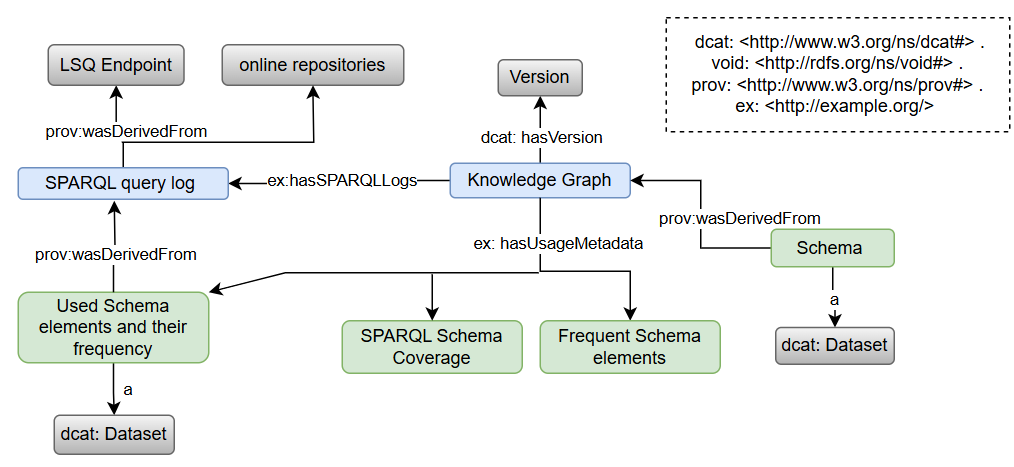
\includegraphics[width=0.8\textwidth]{image16.png}
    \caption{Usage metadata model.}
    \label{fig:l9}
\end{figure}


\subsubsection{Utility: usage metadata predicts demand better than KG content in this setting}\label{sec:utility}

The preceding analyses point to a concrete application: a type-suggestion feature for a query builder, of the kind a KG maintainer might deploy. We evaluate it as a temporal ranking task to test whether the usage metadata is useful for prioritizing future demand. We rank Wikidata schema types by their class-position usage frequency in the \emph{early-2017} organic logs (the ``training'' period), and measure what fraction of the class-type demand in the \emph{2018} organic log (the ``test'' period, approximately eight months later) is captured by the top-$k$ suggestions. Following the rest of our frequency analysis (Section~\ref{s4}), demand is computed over unique (deduplicated) queries, so that a single heavily repeated example or tool query cannot dominate the evaluation.

As a simple content-based baseline, we rank the same types by KG \emph{supply}, measured as the number of instances per class in the 2017 dump. This provides a ranking derived from the KG itself, without using query-log information, and allows us to compare usage-based prioritization with a readily available content signal.

\DIFaddbegin \DIFadd{We should be explicit about how this relates to existing autocompletion work, because the comparison we run is narrower than that literature. Dedicated SPARQL autocompletion systems already rank suggestions, and do so with machinery we do not attempt to match: Bast et al.~\mbox{%DIFAUXCMD
\cite{bast2022autocompletion} }\hskip0pt%DIFAUXCMD
evaluate context-sensitive and context-agnostic ranked autocompletion on Wikidata at interactive latencies, and de la Parra and Hogan~\mbox{%DIFAUXCMD
\cite{delaparra2021autocompletion} }\hskip0pt%DIFAUXCMD
derive suggestions from KG structure with approximate, content-derived ranking signals. Both rank against the KG (and, in the context-sensitive case, against the partially written query); neither draws on what users have historically queried, because query-log usage statistics of the kind we generate have not been available to them. Our experiment is therefore not a system comparison and should not be read as one. It isolates a single question those systems leave open: given a ranking problem they already solve from KG-side signals, how much is added by a signal derived from past usage? The content-based supply ranking stands in for the KG-side signal in its simplest form, so the gap we measure is a lower bound on what a usage-aware ranker could contribute to a system such as theirs, not a claim to outperform one. Integrating usage priors into a full autocompletion system, and evaluating them against these baselines under their latency constraints, is the natural follow-up.
}

\DIFaddend \begin{table}[ht]
\centering
\caption{Percentage of 2018 organic class-type demand (deduplicated) captured by the top-$k$ suggested types, ranked by past (2017) usage or by KG supply (instances/class).}
\label{tab:utility}
\begin{tabular}{r|r|r}
\hline
Top-$k$ suggestions & Ranked by past usage & Ranked by KG supply \\
\hline
10   & 40.3\% & 32.1\% \\
50   & 54.1\% & 42.3\% \\
100  & 61.7\% & 49.0\% \\
500  & 75.7\% & 62.5\% \\
1000 & 79.9\% & 68.1\% \\
\hline
\end{tabular}
\end{table}

Figure~\ref{fig:utility} and Table~\ref{tab:utility} show the result. A list of the 50 most-used types in 2017 covers \textbf{54\%} of the deduplicated class-type demand observed eight months later, rising to approximately 80\% at top-1000. The content-based ranking performs consistently worse: its top-50 covers \textbf{42\%}, and it requires \textbf{148 suggestions} to match the coverage achieved by the top 50 types in the usage-based ranking. This difference is consistent with the content--demand relationship observed in Section~\ref{sec:classvalue}. Several of the highest-supply classes, including \emph{scholarly article}, \emph{Wikimedia category}, \emph{taxon}, \emph{disambiguation page}, \emph{Wikimedia template}, \emph{gene}, and \emph{protein}, appear relatively infrequently in the organic query log, whereas the usage-ranked list places frequently queried classes such as \emph{human}, \emph{film}, \emph{city}, \emph{country}, \emph{human settlement}, \emph{university}, and \emph{business} near the top.

Top-$k$ coverage measures how much future demand is captured by the suggestion set, but it is insensitive to the ordering of items within that set. Since the position of an item is also relevant in a ranked suggestion list, we additionally evaluate the same split using nDCG@$k$, with graded relevance given by each type's deduplicated 2018 demand, and a demand-weighted mean reciprocal rank,
$\mathrm{MRR}_w = \sum_t (d_t / r_t) / \sum_t d_t$,
where $d_t$ is the 2018 demand for type $t$ and $r_t$ its rank in the suggestion list.

\begin{table}[ht]
\centering
\caption{Order-sensitive evaluation of the type-suggestion task using the same train/test split as Table~\ref{tab:utility}. nDCG@$k$ uses graded relevance equal to each type's deduplicated 2018 demand; $\mathrm{MRR}_w$ is demand-weighted mean reciprocal rank over the full ranking.}
\label{tab:ranking}
\begin{tabular}{r|r|r}
\hline
Top-$k$ & nDCG@$k$ (past usage) & nDCG@$k$ (KG supply) \\
\hline
10   & 94.9\% & 44.5\% \\
50   & 94.1\% & 46.3\% \\
100  & 93.8\% & 47.2\% \\
500  & 92.7\% & 48.6\% \\
1000 & 92.5\% & 49.3\% \\
\hline
\multicolumn{3}{l}{$\mathrm{MRR}_w$: past usage $0.338$ \quad KG supply $0.117$ \quad (ratio $2.9\times$)} \\
\hline
\end{tabular}
\end{table}

The order-sensitive evaluation shows an even larger difference between the two rankings. The usage ranking achieves nDCG@10 of \textbf{94.9\%}, compared with \textbf{44.5\%} for the supply ranking, and remains above 92\% through $k=1000$. Demand-weighted MRR shows the same pattern ($0.338$ versus $0.117$). Thus, the usage-based ranking not only captures more subsequently observed demand within its top positions, but also places the more frequently demanded types closer to the top.

The experiment covers one KG, one schema-element type, and one temporal split, so the result should be interpreted within this setting rather than as evidence that usage metadata generally forecasts future demand. Within this setting, however, the difference between the two rankings is stable under query-level bootstrap resampling. Across 2{,}000 resamples of the 185{,}443 test queries, the usage-minus-supply coverage gap remains positive at every evaluated list length. At top-50, the difference is $+11.8$ percentage points (95\% CI $[11.2,12.4]$), and at top-1000 it is also $+11.8$ points (95\% CI $[11.3,12.4]$). Broader evaluation across additional KGs, schema-element types, and time periods remains future work.

\begin{figure}
    \centering
    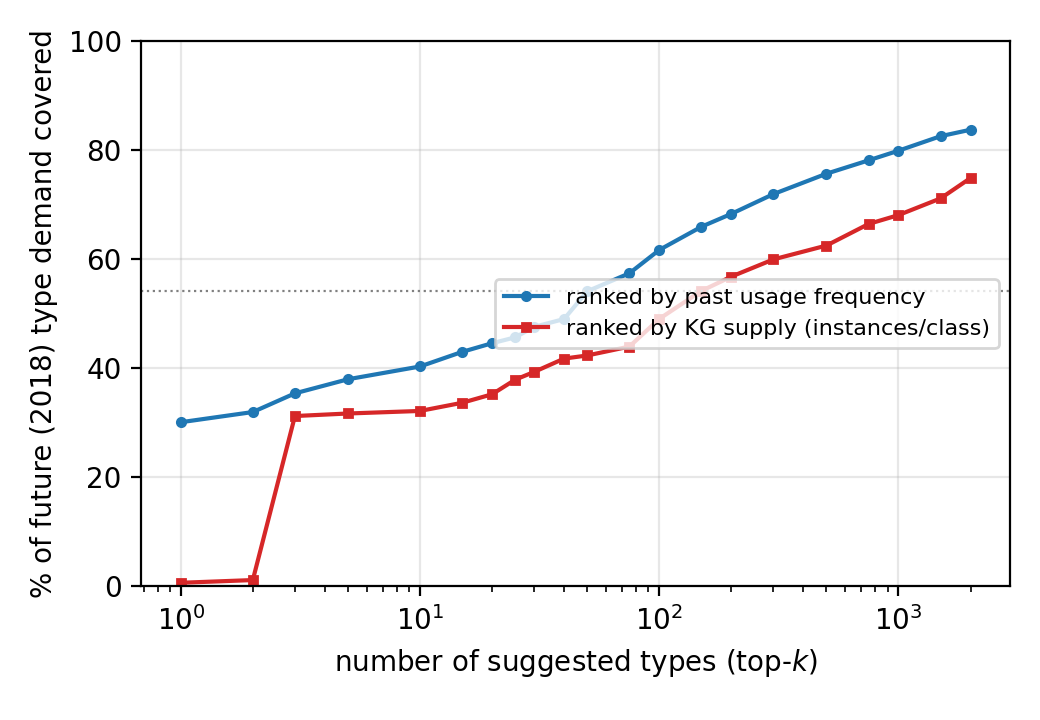
\includegraphics[width=0.62\textwidth]{utility_autocomplete.png}
    \caption{Future class-type demand covered by the top-$k$ suggestions when Wikidata types are ranked by their 2017 usage frequency or by KG supply in instances per class.}
    \label{fig:utility}
\end{figure}

\DIFdelbegin %DIFDELCMD < \begin{comment}%DIFDELCMD < 
%DIFDELCMD <     If this experiment is intended to demonstrate the practical utility of usage metadata for autocomplete, I think the evaluation should be better connected to existing SPARQL-autocomplete work. Using class size as a simple content-based baseline is reasonable, and content-derived signals have also been used in previous autocomplete approaches. However, there are more closely related methods that explicitly rank autocomplete suggestions. For example, Bast et al., *Efficient and Effective SPARQL Autocompletion on Very Large Knowledge Graphs* (CIKM 2022), evaluate ranked context-sensitive and context-agnostic autocomplete on Wikidata, while de la Parra and Hogan, *Fast Approximate Autocompletion for SPARQL Query Builders* (2021), derive autocomplete suggestions from KG structure and use content-based ranking signals. It would therefore be useful to compare the proposed usage-based ranking with such approaches where feasible, or at least position the present experiment with respect to them and clarify what additional role usage metadata could play. Otherwise, the experiment may be better framed more narrowly as showing that historical usage provides a useful alternative to a simple KG-content ranking, rather than as demonstrating utility for autocomplete more generally. It is also unclear why only type/class suggestions are evaluated, while the generated usage metadata also covers predicates and predicate suggestion is equally relevant to SPARQL autocomplete. Either predicate ranking should also be evaluated or the restriction to classes should be acknowledged and presented as a demonstration.  
%DIFDELCMD < 
%DIFDELCMD < \end{comment}
%DIFDELCMD < %%%
\DIFdelend \DIFaddbegin \paragraph{\textbf{\DIFadd{Predicate suggestion.}}}
\DIFadd{The evaluation above ranks types, but the usage metadata covers predicates too, and predicate
suggestion matters at least as much in a query builder. We therefore repeated the experiment over
predicates, with the same train/test split and the content-side analogue of instances-per-class,
namely triples per predicate in the 2017 dump (Table~\ref{tab:predranking}). Usage again wins, but
by a visibly smaller margin than for types, and the gap closes as the list grows: nDCG@10 is 85.9\%
against 58.6\%, and top-10 demand coverage 43.3\% against 23.0\%, yet by top-1000 the two rankings
are nearly indistinguishable (94.8\% vs 93.3\%). Demand-weighted MRR is $0.258$ against $0.202$, a
$1.3\times$ ratio rather than the $2.9\times$ seen for types.
}\DIFaddend 

\DIFaddbegin \DIFadd{The asymmetry is informative rather than disappointing, and it has a straightforward explanation.
Wikidata has roughly a thousand predicates against a hundred thousand classes, so a content-ranked
predicate list runs out of room to be wrong: even an indifferent ordering reaches most of the demand
within a few hundred suggestions. The content--demand inversion of Section~\ref{sec:classvalue} is
also specifically a class-side pathology, driven by bulk- and bot-imported categories that carry
enormous instance counts and attract no queries; predicates have no comparable population of
heavily-instantiated-but-unqueried members. Usage metadata therefore helps most exactly where the
content signal is weakest, which is on the class side. Reporting only the type experiment would have
overstated how uniform that benefit is.
}

\begin{table}[ht]
\centering
\caption{\DIFaddFL{Predicate-suggestion counterpart to Table~\ref{tab:ranking}, same train/test split. Predicates are ranked by past usage or by KG supply (triples per predicate). The usage advantage is real but smaller than for types, and narrows as $k$ grows.}}
\label{tab:predranking}
\begin{tabular}{r|r|r|r|r}
\hline
Top-$k$ & nDCG@$k$ (past usage) & nDCG@$k$ (KG supply) & Coverage (usage) & Coverage (supply) \\
\hline
10   & 85.9\% & 58.6\% & 43.3\% & 23.0\% \\
50   & 90.4\% & 67.1\% & 73.1\% & 54.3\% \\
100  & 90.9\% & 72.6\% & 81.4\% & 72.5\% \\
500  & 91.3\% & 75.3\% & 92.3\% & 88.7\% \\
1000 & 91.6\% & 76.1\% & 94.8\% & 93.3\% \\
\hline
\multicolumn{5}{l}{$\mathrm{MRR}_w$: past usage $0.258$ \quad KG supply $0.202$ \quad (ratio $1.3\times$)} \\
\hline
\end{tabular}
\end{table}



\DIFaddend \section{Discussion}\label{s5}
In this study, we analyzed SPARQL query logs to explore how users interact with knowledge graphs (KGs) by addressing two key questions: (1) How can we quantify the usage of a KG? and (2) Do frequency distribution and ranking analyses of used KG elements reveal usage patterns over different log intervals or across organic (human-driven) and robotic (bot-driven) query types? We applied the proposed method to the both robotic and organic query logs from Bio2RDF and Wikidata, uncovering several patterns in schema element usage.

To quantify the overall usage of a KG, we introduced the SPARQL schema coverage metric, which measures the proportion of schema elements that are explicitly referenced in queries. Raw coverage differs markedly between robotic and organic logs (robotic 97\% for Bio2RDF and 60\% for Wikidata; organic 21\% and 14\%), which might suggest that automated processes simply access a broader range of the schema. However, robotic and organic logs also differ in size by up to two orders of magnitude, so raw coverage conflates breadth of interest with sheer query volume. The size-controlled rarefaction analysis (Section~\ref{sec:rarefaction}) separates the two, and the outcome differs between the two datasets rather than supporting a blanket statement about ``machine vs.\ human'' querying. In Bio2RDF, a relatively compact biomedical KG, the robotic logs \DIFdelbegin \DIFdel{still cover roughly $1.8\times$ }\DIFdelend \DIFaddbegin \DIFadd{cover no }\DIFaddend more of the schema than the organic logs at equal sampling effort \DIFdelbegin \DIFdel{, so the coverage }\DIFdelend \DIFaddbegin \DIFadd{($0.88\times$, 95\% CI $[0.75, 1.02]$), so the raw }\DIFaddend difference there is \DIFdelbegin \DIFdel{not }\DIFdelend explained by sample size\DIFdelbegin \DIFdel{alone}\DIFdelend . In Wikidata the difference essentially vanishes at equal effort, and organic queries are richer per occurrence at small samples; the large raw gap is largely attributable to volume, amplified by a long tail of one-off references (two thirds of robotic Wikidata elements are used exactly once). We draw the methodological lesson rather than a structural one: schema coverage must be interpreted relative to sampling effort, and a raw coverage gap between query types cannot be read as behavioral without an equal-effort comparison. With two KGs we cannot attribute the differing outcomes to schema scale as such, since the two systems also differ in domain, user community, and workload; whether the pattern tracks scale is a question for the broader study we call for in Section~\ref{s5}.

Beyond coverage, we observed a pronounced long-tail distribution in the frequency of schema element usage in both datasets. While a few schema elements are queried very frequently, the vast majority are rarely used. We made this precise with concentration statistics (Section~\ref{sec:concentration}, Table~\ref{tab:concentration}): the Gini coefficient of usage exceeds \DIFdelbegin \DIFdel{0.90 }\DIFdelend \DIFaddbegin \DIFadd{0.91 }\DIFaddend in every dataset \DIFaddbegin \DIFadd{except the very sparse }\emph{\DIFadd{Bio2RDF-organic-2019}} \DIFadd{log, }\DIFaddend and as little as 0.1--4\% of used elements account for 80\% of all references. This matters for how coverage should be read: a high coverage number reports that nearly every element is touched at least once, which is almost the opposite of demand being spread evenly across the schema. This long-tail phenomenon is significant because it demonstrates that only a limited set of elements captures most of the user attention, despite the overall diversity in accessed elements. Schema coverage and usage concentration are therefore complementary rather than redundant, the breadth of elements accessed versus how unequally that breadth is exercised, and together they provide a comprehensive view of usage patterns without implying a direct causal relation between them. An information-theoretic or inequality measure (entropy, Gini) is the right summary when the question is ``how concentrated is demand,'' and coverage when the question is ``how much of the schema is reached at all.''

We computed Spearman’s rank correlations based on the frequency rankings of common schema elements in dataset pairs. Over a longer time span (e.g., Bio2RDF All logs: 2013 vs. 2019), the weak correlation suggests shifting rankings over time. In contrast, moderate correlation in shorter intervals of Wikidata robotic logs (2017 vs. 2018) and Wikidata organic logs (2017 vs. 2018), indicates greater consistency in the near term.

Focusing on the most frequently queried schema types, our findings reveal a dual pattern in both the top 10 and top 50 elements. In the top 10 analysis, a small stable core, typically comprising 2 to 4 elements, appears consistently across different datasets, time intervals, and query types, while the remaining elements tend to vary. In the top 50 frequent elements, we observe an overlap of 24\% to 46\% common elements across different comparisons. This indicates that although a core set of schema elements remains persistently frequent (likely due to their fundamental role or inherent relevance), the majority of frequently queried elements are variable, reflecting evolving user interests or updates in data structures. Importantly, the persistent core can be leveraged in KG documentation and design, ensuring that these key elements are prioritized and optimized to better serve user needs.

% Taken together, these findings provide a nuanced view of KG usage patterns. Both organic and robotic queries exhibit a long-tail distribution in schema element usage; however, robotic queries access a broader range of elements, while organic queries concentrate on a smaller subset. Recognizing this distinction is important because it reveals that, despite similar overall distributions, the type of query (automated vs. human-driven) influences the breadth of schema elements used. Furthermore, the presence of a stable core in the top 10—coupled with substantial variability in the remaining elements—and the Spearman’s rank correlation results highlight a dual pattern of stability and evolution in KG usage. Short-term consistency exists among the most frequently queried elements, while longer time spans witness more substantial reordering in element popularity. These insights offer valuable perspectives for optimizing knowledge graph design and query strategies to better cater to diverse user needs.

In addition, the pairwise schema type co-occurrence analysis in Bio2RDF reveals that the number of distinct cross-subgraph join patterns observed in queries increased from 3 in the 2013 logs to 22 in the 2019 logs. This increase indicates that queries combined data from multiple Bio2RDF datasets more often in 2019 than in 2013. A likely contributing factor is improved accessibility, in particular the shift from a separate endpoint per dataset in 2013 to a single unified endpoint in 2019, which removes the need to federate across endpoints in order to join two datasets. These results demonstrate the importance of designing KGs that support robust federated query capabilities, especially in data-driven fields like bioinformatics.

Together, these findings describe a consistent picture of the logs we analysed: usage is heavily concentrated on a small set of schema elements, that set is largely stable from one interval to the next, raw coverage differences between query types are driven substantially by log size, and on an item-based KG a sizeable share of apparent class usage is in fact value usage. Each of these bears directly on how KG documentation, interface design, and deprecation decisions should be prioritised.

This study has several limitations, which also point to future work.

\emph{Comparability of the two KGs.} The log collection periods differ (Bio2RDF $\sim$30 months vs.\ Wikidata $\sim$9 months) and the schemas differ in scale by roughly two orders of magnitude. We mitigate the first with time-normalized counts and the second by reporting coverage primarily within each KG and by the size-controlled rarefaction analysis; nonetheless, cross-KG coverage percentages should not be read as a direct ranking. For the within-Wikidata temporal comparison, the original analysis compared just two intervals (2017 and 2018); we additionally verified that result against seven consecutive equal-length (28-day) windows (Section~\ref{sec:equalintervals}), confirming that coverage ($\sim$4\%) and rank stability ($\rho \approx 0.47$--$0.51$) are not artifacts of the particular pair of intervals chosen. Direct comparison across KGs of similar scale remains valuable future work.

\emph{Schema coverage does not transfer cleanly from an OWL-style KG to an item-based one.}
This is the study's most consequential lesson, and it emerged from extending a metric
designed for Bio2RDF to Wikidata. In Bio2RDF, classes and predicates are OWL-style
vocabulary terms and ``coverage'' is well defined. In Wikidata there is no formal
class/instance separation; ``classes'' are ordinary items, and, as Section~\ref{sec:classvalue}
shows, a large share of the items counted as queried types (about 30\% in human
queries) are referenced only as property \emph{values}, never as classes. A single
coverage percentage therefore conflates value usage with schema usage, and the Bio2RDF
and Wikidata figures are not directly comparable: the lower Wikidata coverage is partly
definitional, not purely behavioral. For item-based KGs, a faithful usage measure must
(i) separate class-position from value-position references and (ii) restrict to
instantiated classes. The content--demand inversion (Section~\ref{sec:classvalue}, Figure~\ref{fig:mismatch})
sharpens the point: Wikidata's most heavily instantiated classes, bulk- and
bot-imported geographic, biological, and structural categories, attract almost no
query demand, while demand concentrates on a small, intuitive class core and on items
queried as values. This also refines the organic/robotic contrast: human queries reference
type-items as values far more than bots do (which traverse them as classes), so human
``coverage'' is the more inflated of the two. A third KG, DBpedia, isolates the size effect:
it is as large and broad as Wikidata but OWL-style like Bio2RDF, and only 6.5\% of its
queried classes are value-only (Table~\ref{tab:generality}), with the same content--demand
inversion (heavily instantiated \emph{Tenure}/\emph{WikimediaTemplate} unqueried; demand on
\emph{Place}/\emph{Person}/\emph{Film}). Across these three KGs, then, value-position inflation
appears to be associated with the modeling style rather than with KG size or breadth, and the
content--demand inversion is present under both styles. We state this as an observation about
the systems we examined: three KGs cannot establish that the association holds generally, and
a KG with different conventions could well behave otherwise.
Residual caveats remain, \texttt{wdt:P279}
has subproperties we do not follow, and a principled, instance-aware notion of ``class''
for Wikidata is an open problem \cite{brasileiro2016applying,piscopo2018who,patelschneider2024class}, but the broader message is that usage metrics must be matched to a KG's modeling style.

\emph{Explicit vs.\ semantic (effective) usage.} We measure \emph{explicit} usage: a schema element is used when it is explicitly written in a query. This is the right notion for documentation, interface, and deprecation decisions, but it is not the same as a \emph{semantic} (effective) notion that would also credit the subclasses and subproperties a property path (e.g.\ \texttt{wdt:P31/wdt:P279*}) traverses at evaluation time and that also contribute to answers. As we show in Section~\ref{s3}.4, a naive closure-based notion is in fact \emph{ill-behaved} on an item-based KG: because users occasionally anchor \texttt{wdt:P279*} at near-root classes such as \emph{entity}, crediting the full subclass closure would mark $\sim$62\% of all Wikidata classes as ``used,'' driven by a handful of queries. A useful effective-usage measure would therefore need to attribute usage \emph{partially} (e.g.\ weighting by how many traversed elements actually contribute answers, or capping anchor generality) rather than crediting the whole closure; designing such a measure is a natural and substantial extension.

\emph{Example-query contamination and weighting.} ``Organic'' logs can be contaminated by demonstration and example queries. We measured this directly against the period's Wikidata Query Service example set (Section~\ref{sec:equalintervals}'s frequent-types discussion): verbatim example runs are only $\sim$1.4\% of executions and do not change the coverage or top-type results. This is a lower bound, it does not capture example queries that users \emph{adapt} before running (e.g.\ swapping the occupation or class in a template), which a fuzzier, subpattern-based matcher could estimate. Complementing our deduplicated (intent-diversity) counts with volume-weighted counts, and detecting adapted-example traffic, would further sharpen the behavioral interpretation.

\emph{Organic vs.\ robotic is a user-agent proxy, not a ground truth.} The organic/robotic partition we use (Section~\ref{s1}) is the established user-agent--based classification of \cite{malyshev2018getting,bielefeldt2018practical}: browser-like agents are labelled organic, the remainder robotic. This is a coarse proxy. Notebook kernels, programmatic API clients, browser extensions, and increasingly LLM-driven agents do not map cleanly onto ``human vs.\ bot,'' and a determined client can spoof any user-agent string, so ``robotic'' is more precisely read as ``non-browser client'' than as ``automated, non-human.'' We mitigate over-reliance on the label in two ways: our central conclusions are reported \emph{within} each class and the size-controlled analysis (Section~\ref{sec:rarefaction}) guards against reading a raw coverage gap as behavioral, and we note that the two classes also differ syntactically in these logs, the vendor-specific full-text and \texttt{OPTION} syntax concentrating in organic traffic (Section~\ref{s4}.3), although as noted there that contrast may reflect the web-form access path rather than an inherent human/automated distinction. Still, the partition should be treated as an informative but imperfect signal, and a classification that incorporates query content or session structure is an avenue for future refinement.

\emph{Scope: an exploratory study across contrasting modeling styles.} We deliberately position this work as an exploratory study across a small number of deliberately contrasting KG architectures: the OWL-style biomedical Bio2RDF and the item-based encyclopedic Wikidata, with DBpedia as a third point that separates modeling style from scale, rather than as a universal characterisation of KG usage. The headline patterns (extreme usage concentration, a stable queried core, value-position inflation tracking modeling style, and the content--demand inversion) are consistent across these systems, but confirming that they hold for other large public endpoints with their own conventions, e.g.\ UniProt, ChEMBL, OpenAlex, Europeana, or government data portals, and for KGs of similar scale but differing style, remains important future work that requires access to their query logs.

\emph{Toward demand-aware governance and execution-aware usage.} Two extensions would tighten the bridge to KG maintenance. First, our supply--demand analysis (Section~\ref{sec:classvalue}) identifies schema elements that are heavily populated yet rarely queried; pairing this with a \emph{maintenance-cost} signal (e.g.\ update frequency, provenance complexity, or storage footprint per class) would let maintainers target review at elements that are expensive to keep current but attract little demand, a direct input to deprecation and curation decisions. Second, our usage notion is binary (an element is referenced or not). A richer, execution-aware hierarchy: referenced, executed, executed successfully, and actually contributing to returned results, would distinguish these increasingly stringent notions of ``use''; the LSQ-derived logs we work with do not carry result-set, so this requires instrumented endpoints and is left to future work.


\section{Conclusion}\label{s6}
This study introduces a novel approach for analyzing SPARQL query logs to gain deeper insights into user interactions with KGs. To identify usage patterns, we introduce the SPARQL schema coverage metric and conduct frequency distribution and ranking analyses of queried KG elements across different log intervals and both organic and robotic query types from Bio2RDF and Wikidata.
The findings reveal that both query types in both datasets exhibit a long-tail distribution in schema element usage. Raw coverage is higher for robotic queries (60--97\%) than organic ones (13--21\%), but a size-controlled (rarefaction) analysis shows that \DIFdelbegin \DIFdel{this gap persists after controlling for sampling effort only for Bio2RDF; for Wikidata it is largely a consequence of robotic logs being far larger}\DIFdelend \DIFaddbegin \DIFadd{in neither KG does the gap survive once sampling effort is equalized, so it chiefly reflects the far greater volume of robotic traffic}\DIFaddend . A further, central finding is that schema coverage does not transfer cleanly between KGs of different modeling styles: on the item-based Wikidata, roughly 30\% of the items counted as queried ``classes'' in human queries are in fact used as property values, and the most heavily instantiated classes are rarely queried, a structural mismatch between KG content and query demand that a single coverage percentage obscures. A third KG, DBpedia, indicates that this value-position inflation is associated with the modeling style (item-based vs.\ OWL) rather than with KG size, while the content--demand inversion is present under both styles. With three KGs these are reported observations rather than established regularities. The same modeling difference makes a naive closure-based notion of ``effective usage'' ill-behaved on Wikidata, where a handful of queries anchored at near-root classes would mark most of the ontology as used, evidence that explicit reference is the appropriate primitive for an item-based KG.
The temporal analysis identifies a stable core of elements that consistently drive user queries over time; across seven consecutive equal-length intervals the organic coverage and the element-ranking correlation are stable, confirming that this is not an artifact of which two endpoints are compared, while over the six-year Bio2RDF span rankings shift more. Finally, we demonstrate that this usage metadata has concrete predictive value: a type-suggestion ranking learned from one year of logs captures most of the next year's query demand and substantially outperforms a ranking by KG content, which wastes its top suggestions on bulk-imported but unqueried classes.
Overall, our findings advance the understanding of KG usage patterns and provide guidance for optimizing KG design, documentation, and query strategies, ultimately contributing to the development of more responsive and user-centric knowledge graphs.

The implementation of this method is publicly available on the GitHub repository: \url{https://github.com/MaastrichtU-IDS/KG_usage_metadata}.
\DIFdelbegin %DIFDELCMD < 

%DIFDELCMD < \begin{comment}%DIFDELCMD < 
%DIFDELCMD <     The following comments relate to the GitHub repository, and the repository should be updated accordingl:
%DIFDELCMD <     1.Some of the datasets used in the experiments are not directly included in the repository, which is understandable given their large size. However, the repository should provide clear information on how these datasets can be obtained. In particular, several scripts reference input files under data/... (e.g., data/logs/dbpedia/dbpedia_texts.txt, containing the distinct executed DBpedia query texts), but no download link, source, or instructions are provided for accessing these data. Providing references to the original data source or download location is essential to support reproducibility.
%DIFDELCMD <     Also make a refrence that shows which script created each figures of the manuscript. e.g Figure 9 ---> script1.py 
%DIFDELCMD <     
%DIFDELCMD <     2. Initially, it was unclear whether the updated preprocessing was applied only to Bio2RDF, since the repository states that it replaces `Schema_coverage_calculation_BIO2RDF.ipynb` from the previous repository, and the new implementation is named `parse_validate_bio2rdf2019.py`. After reviewing the code, it appears that the same preprocessing pipeline is also used for Wikidata and DBpedia. However, naming a general preprocessing script `parse_validate_bio2rdf2019.py` is misleading, as it suggests that the implementation is specific to the Bio2RDF dataset. A more general and descriptive filename would better reflect its purpose and improve the repository's clarity and maintainability.
%DIFDELCMD <     
%DIFDELCMD <     3.The scripts `wd_closure_bound.py` and `wd_closure_anchors.py` provide partial support for the closure-based claim. `wd_closure_bound.py` computes the combined subclass closure of classes used as anchors in `wdt:P279*` or `wdt:P279+` paths, while `wd_closure_anchors.py` reports the broad anchor classes, the number of queries in which each anchor occurs, and the size of its subclass closure.
%DIFDELCMD <     However, two aspects of the manuscript’s claim are not directly reproducible from the reported script outputs. First, the manuscript states that approximately 62% of all Wikidata classes would be marked as used, whereas `wd_closure_bound.py` reports the additional closure-derived classes as a percentage of TSE, whose denominator includes both classes and predicates. Second, although `wd_closure_anchors.py` reports how many queries use each near-root anchor, neither script prints or saves the actual query texts constituting the claimed “handful of queries.” The repository should explicitly compute the percentage relative to the Wikidata class universe and provide the specific queries responsible for the near-root anchors, so that both parts of the claim can be verified.
%DIFDELCMD <     
%DIFDELCMD <     4.The GitHub reposository has a specific readme file for this analysis, which is a great, in this readme we can see the data Source is accesssible from: Wikidata:SPARQL_query_service/queries/examples, revision 509986548 (timestamp 2017-06-30T00:32:28Z), the latest revision before the organic log period. I sugesst we add the link for retrieving this resource as well: https://www.wikidata.org/w/index.php?title=Wikidata:SPARQL_query_service/queries/examples&oldid=509986548 
%DIFDELCMD <     It would be excellent if all other analyses had such documentation/readme file. 
%DIFDELCMD < 
%DIFDELCMD <     5.Potential issue in dbpedia_analysis.py: The correctness of the parallel result ordering is not obvious. Since query frequencies are associated with parsed results after parallel processing, it would be useful to verify that worker output order matches the original query order.
%DIFDELCMD <     Suggested test: Run the analysis on a small sample with nw=1 and nw>1 and confirm that all frequency-based outputs (especially cls_dem and class-demand rankings) are identical.
%DIFDELCMD < 
%DIFDELCMD < \end{comment}
%DIFDELCMD < %%%
\DIFdelend 


\section{Acknowledgment}\label{s7}
This project has received funding from the European Union’s Horizon 2020 research and innovation program under the Marie Skłodowska-Curie grant agreement No 860801.

%\subsection{}\label{s1.1}

%\begin{figure}[t]
%\includegraphics{}
%\caption{Figure caption.}\label{f1}
%\end{figure}

%\begin{table*}
%\caption{} \label{t1}
%\begin{tabular}{lll}
%\hline
%&&\\
%&&\\
%\hline
%\end{tabular}
%\end{table*}

%%%%%%%%%%% The bibliography starts:

%%%%%%%%%%%%%%%%%%%%%%%%%%%%%%%%%%%%%%%%%%%%%%%%%%%%%%%%%%%%%
%%                  The Bibliography                       %%
%%                                                         %%
%%  ios1.bst will be used to                               %%
%%  create a .BBL file for submission.                     %%
%%                                                         %%
%%                                                         %%
%%  Note that the displayed Bibliography will not          %%
%%  necessarily be rendered by Latex exactly as specified  %%
%%  in the online Instructions for Authors.                %%
%%                                                         %%
%%%%%%%%%%%%%%%%%%%%%%%%%%%%%%%%%%%%%%%%%%%%%%%%%%%%%%%%%%%%%


\nocite{*}
% if your bibliography is in bibtex format, use those commands:
\bibliographystyle{ios1}           % Style BST file.
\bibliography{bibliography}        % Bibliography file (usually '*.bib')

% or include bibliography directly:
%\begin{thebibliography}{0}
%\bibitem{r1} F. Author, Information about cited object.
%
%\bibitem{r2} S. Author and T. Author, Information about cited object.
%\end{thebibliography}
% \begin{thebibliography}{0}

% \bibitem{1} B. Abu-Salih, \textit{Domain-specific knowledge graphs: A survey}, \textit{Journal of Network and Computer Applications} \textbf{185} (2021), 103076.

% \bibitem{2} W. Ali, M. Saleem, B. Yao, A. Hogan, and A.-C. Ngonga Ngomo, \textit{A survey of RDF stores \& SPARQL engines for querying knowledge graphs}, \textit{The VLDB Journal} (2022), 1-26.

% \bibitem{3} L. Asprino and M. Ceriani, \textit{How is Your Knowledge Graph Used: Content-Centric Analysis of SPARQL Query Logs}, in: \textit{International Semantic Web Conference}, Springer Nature Switzerland, 2023, pp. 197-215.

% \bibitem{4} A. Bielefeldt, J. Gonsior, and M. Krötzsch, \textit{Practical Linked Data Access via SPARQL: The Case of Wikidata}, in: \textit{LDOW@WWW}, 2018.

% \bibitem{5} A. Bonifati, W. Martens, and T. Timm, \textit{An analytical study of large SPARQL query logs}, \textit{The VLDB Journal} \textbf{29}(2) (2020), 655-679.

% \bibitem{6} C. Buil-Aranda, M. Ugarte, M. Arenas, and M. Dumontier, \textit{A preliminary investigation into SPARQL query complexity and federation in Bio2RDF}, in: \textit{Alberto Mendelzon International Workshop on Foundations of Data Management}, 2015, p. 196.

% \bibitem{7} M. Saleem, M. I. Ali, A. Hogan, Q. Mehmood, and A.-C. Ngonga Ngomo, \textit{LSQ: the linked SPARQL queries dataset}, in: \textit{The Semantic Web-ISWC 2015: 14th International Semantic Web Conference}, Springer International Publishing, 2015, pp. 261-269.

% \bibitem{8} C. Stadler, M. Saleem, Q. Mehmood, C. Buil-Aranda, M. Dumontier, A. Hogan, and A.-C. Ngonga Ngomo, \textit{LSQ 2.0: A linked dataset of SPARQL query logs}, \textit{Semantic Web Preprint} (2024), 1-23.

% \bibitem{9} \url{https://www.npmjs.com/package/sparqljs}.

% \bibitem{10} F. Belleau, M.-A. Nolin, N. Tourigny, P. Rigault, and J. Morissette, \textit{Bio2RDF: towards a mashup to build bioinformatics knowledge systems}, \textit{Journal of Biomedical Informatics} \textbf{41}(5) (2008), 706-716.

% \bibitem{11} A. Hogan, E. Blomqvist, M. Cochez, C. d’Amato, G. De Melo, C. Gutierrez, S. Kirrane, et al., \textit{Knowledge graphs}, \textit{ACM Computing Surveys (Csur)} \textbf{54}(4) (2021), 1-37.

% \bibitem{12} M. Mohammadi, \textit{(Semi-) Automatic Construction of Knowledge Graph Metadata}, in: \textit{European Semantic Web Conference}, Springer International Publishing, 2022, pp. 171-178.

% \bibitem{14} M. Mohammadi, and M. Dumontier,\textit{ Analyzing SPARQL Query Logs: A Study on Schema Coverage and Query Content}, \textit{Semantic Web Applications and Tools for Health Care and Life Sciences (SWAT4HCLS)}, 2024, \url{https://ceur-ws.org/Vol-3890/paper-14.pdf}.

% \bibitem{15} K. Möller, M. Hausenblas, R. Cyganiak, S. Handschuh, and G.A. Grimnes, \textit{Learning from Linked Open Data Usage: Patterns \& Metrics}, in: \textit{Proc. Web Science Conf. (WebSci’10)}, 2010.

% \bibitem{16} A. Bonifati, W. Martens, and T. Timm, \textit{An Analytical Study of Large SPARQL Query Logs}, \textit{Proceedings of the VLDB Endowment} \textbf{11}(2017), 149–161, Issue 2.

% \bibitem{17} M. Kaminski and E.V. Kostylev, \textit{Complexity and Expressive Power of Weakly Well-Designed SPARQL}, \textit{Theory of Computing Systems} (2018), 1–38, \url{https://doi.org/10.1007/s00224-017-9802-9}.

% \bibitem{18} F. Picalausa and S. Vansummeren, \textit{What are real SPARQL queries like?}, in: \textit{Proc. Int.Workshop on SemanticWeb Information Management (SWIM’11)}, ACM, 2011, pp. 6.

% \bibitem{19} J. Lorey and F. Naumann, \textit{Detecting SPARQL Query Templates for Data Prefetching}, in: \textit{Proc. 10th Extended Semantic Web Conference (ESWC’13)}, Springer, 2013, pp. 124–139.

% \bibitem{20} A. Raghuveer, \textit{Characterizing Machine Agent Behavior through SPARQL Query Mining}, in: \textit{Proc. 2nd Int. Workshop on Usage Analysis and the Web of Data (USEWOD’12)}, 2012.

% \bibitem{21} L. Rietveld and R. Hoekstra, \textit{Man vs. Machine: Differences in SPARQL Queries}, in: \textit{Proc. 4th USEWOD Workshop on Usage Analysis and the Web of Data}, 2014.

% \bibitem{22} C. Peng, F. Xia, M. Naseriparsa, and F. Osborne, \textit{Knowledge graphs: Opportunities and challenges}, \textit{Artificial Intelligence Review} \textbf{56}(11) (2023), 13071-13102.

% \bibitem{23} C. Spearman, \textit{The proof and measurement of association between two things}, (1961).

% \bibitem{24} S. Malyshev, M. Krötzsch, L. González, J. Gonsior, and A. Bielefeldt, \textit{Getting the most out of Wikidata: Semantic technology usage in Wikipedia’s knowledge graph}, in: \textit{The Semantic Web–ISWC 2018: 17th International Semantic Web Conference}, Springer International Publishing, 2018, pp. 376-394.


% \end{thebibliography}


\end{document}

